\documentclass[twoside]{book}

% Packages required by doxygen
\usepackage{fixltx2e}
\usepackage{calc}
\usepackage{doxygen}
\usepackage[export]{adjustbox} % also loads graphicx
\usepackage{graphicx}
\usepackage[utf8]{inputenc}
\usepackage{makeidx}
\usepackage{multicol}
\usepackage{multirow}
\PassOptionsToPackage{warn}{textcomp}
\usepackage{textcomp}
\usepackage[nointegrals]{wasysym}
\usepackage[table]{xcolor}

% Font selection
\usepackage[T1]{fontenc}
\usepackage[scaled=.90]{helvet}
\usepackage{courier}
\usepackage{amssymb}
\usepackage{sectsty}
\renewcommand{\familydefault}{\sfdefault}
\allsectionsfont{%
  \fontseries{bc}\selectfont%
  \color{darkgray}%
}
\renewcommand{\DoxyLabelFont}{%
  \fontseries{bc}\selectfont%
  \color{darkgray}%
}
\newcommand{\+}{\discretionary{\mbox{\scriptsize$\hookleftarrow$}}{}{}}

% Page & text layout
\usepackage{geometry}
\geometry{%
  a4paper,%
  top=2.5cm,%
  bottom=2.5cm,%
  left=2.5cm,%
  right=2.5cm%
}
\tolerance=750
\hfuzz=15pt
\hbadness=750
\setlength{\emergencystretch}{15pt}
\setlength{\parindent}{0cm}
\setlength{\parskip}{3ex plus 2ex minus 2ex}
\makeatletter
\renewcommand{\paragraph}{%
  \@startsection{paragraph}{4}{0ex}{-1.0ex}{1.0ex}{%
    \normalfont\normalsize\bfseries\SS@parafont%
  }%
}
\renewcommand{\subparagraph}{%
  \@startsection{subparagraph}{5}{0ex}{-1.0ex}{1.0ex}{%
    \normalfont\normalsize\bfseries\SS@subparafont%
  }%
}
\makeatother

% Headers & footers
\usepackage{fancyhdr}
\pagestyle{fancyplain}
\fancyhead[LE]{\fancyplain{}{\bfseries\thepage}}
\fancyhead[CE]{\fancyplain{}{}}
\fancyhead[RE]{\fancyplain{}{\bfseries\leftmark}}
\fancyhead[LO]{\fancyplain{}{\bfseries\rightmark}}
\fancyhead[CO]{\fancyplain{}{}}
\fancyhead[RO]{\fancyplain{}{\bfseries\thepage}}
\fancyfoot[LE]{\fancyplain{}{}}
\fancyfoot[CE]{\fancyplain{}{}}
\fancyfoot[RE]{\fancyplain{}{\bfseries\scriptsize Generated by Doxygen }}
\fancyfoot[LO]{\fancyplain{}{\bfseries\scriptsize Generated by Doxygen }}
\fancyfoot[CO]{\fancyplain{}{}}
\fancyfoot[RO]{\fancyplain{}{}}
\renewcommand{\footrulewidth}{0.4pt}
\renewcommand{\chaptermark}[1]{%
  \markboth{#1}{}%
}
\renewcommand{\sectionmark}[1]{%
  \markright{\thesection\ #1}%
}

% Indices & bibliography
\usepackage{natbib}
\usepackage[titles]{tocloft}
\setcounter{tocdepth}{3}
\setcounter{secnumdepth}{5}
\makeindex

% Hyperlinks (required, but should be loaded last)
\usepackage{ifpdf}
\ifpdf
  \usepackage[pdftex,pagebackref=true]{hyperref}
\else
  \usepackage[ps2pdf,pagebackref=true]{hyperref}
\fi
\hypersetup{%
  colorlinks=true,%
  linkcolor=blue,%
  citecolor=blue,%
  unicode%
}

% Custom commands
\newcommand{\clearemptydoublepage}{%
  \newpage{\pagestyle{empty}\cleardoublepage}%
}

\usepackage{caption}
\captionsetup{labelsep=space,justification=centering,font={bf},singlelinecheck=off,skip=4pt,position=top}

%===== C O N T E N T S =====

\begin{document}

% Titlepage & ToC
\hypersetup{pageanchor=false,
             bookmarksnumbered=true,
             pdfencoding=unicode
            }
\pagenumbering{alph}
\begin{titlepage}
\vspace*{7cm}
\begin{center}%
{\Large Term Project\+: Game Delusion }\\
\vspace*{1cm}
{\large Generated by Doxygen 1.8.14}\\
\end{center}
\end{titlepage}
\clearemptydoublepage
\pagenumbering{roman}
\tableofcontents
\clearemptydoublepage
\pagenumbering{arabic}
\hypersetup{pageanchor=true}

%--- Begin generated contents ---
\chapter{Hierarchical Index}
\section{Class Hierarchy}
This inheritance list is sorted roughly, but not completely, alphabetically\+:\begin{DoxyCompactList}
\item Mono\+Behaviour\begin{DoxyCompactList}
\item \contentsline{section}{Box}{\pageref{class_box}}{}
\item \contentsline{section}{Box\+Shield}{\pageref{class_box_shield}}{}
\item \contentsline{section}{Bullet}{\pageref{class_bullet}}{}
\item \contentsline{section}{Button\+Manager}{\pageref{class_button_manager}}{}
\item \contentsline{section}{Camera\+Controller}{\pageref{class_camera_controller}}{}
\item \contentsline{section}{Camera\+Follow2D}{\pageref{class_camera_follow2_d}}{}
\item \contentsline{section}{Chess\+Game\+Control}{\pageref{class_chess_game_control}}{}
\item \contentsline{section}{Door\+Trigger}{\pageref{class_door_trigger}}{}
\item \contentsline{section}{empty}{\pageref{classempty}}{}
\item \contentsline{section}{fly\+Platform}{\pageref{classfly_platform}}{}
\item \contentsline{section}{fly\+Up}{\pageref{classfly_up}}{}
\item \contentsline{section}{Heart}{\pageref{class_heart}}{}
\item \contentsline{section}{Ice\+Platform}{\pageref{class_ice_platform}}{}
\item \contentsline{section}{Lever1}{\pageref{class_lever1}}{}
\item \contentsline{section}{Lives\+Bar}{\pageref{class_lives_bar}}{}
\item \contentsline{section}{Moving\+Object}{\pageref{class_moving_object}}{}
\item \contentsline{section}{New\+Game\+Button}{\pageref{class_new_game_button}}{}
\item \contentsline{section}{Obstacle}{\pageref{class_obstacle}}{}
\item \contentsline{section}{Ornament}{\pageref{class_ornament}}{}
\item \contentsline{section}{Ornament\+Manager}{\pageref{class_ornament_manager}}{}
\item \contentsline{section}{Pause}{\pageref{class_pause}}{}
\item \contentsline{section}{Portal}{\pageref{class_portal}}{}
\item \contentsline{section}{Puzzle}{\pageref{class_puzzle}}{}
\item \contentsline{section}{Quit}{\pageref{class_quit}}{}
\item \contentsline{section}{Reload}{\pageref{class_reload}}{}
\item \contentsline{section}{Shield}{\pageref{class_shield}}{}
\item \contentsline{section}{Show\+Button}{\pageref{class_show_button}}{}
\item \contentsline{section}{Show\+Image}{\pageref{class_show_image}}{}
\item \contentsline{section}{Stair\+Par}{\pageref{class_stair_par}}{}
\item \contentsline{section}{Start\+Position}{\pageref{class_start_position}}{}
\item \contentsline{section}{Test}{\pageref{class_test}}{}
\item \contentsline{section}{the\+End\+Controller}{\pageref{classthe_end_controller}}{}
\item \contentsline{section}{Unit}{\pageref{class_unit}}{}
\begin{DoxyCompactList}
\item \contentsline{section}{Character}{\pageref{class_character}}{}
\item \contentsline{section}{Monster}{\pageref{class_monster}}{}
\begin{DoxyCompactList}
\item \contentsline{section}{Demon}{\pageref{class_demon}}{}
\item \contentsline{section}{Moveable\+Monster}{\pageref{class_moveable_monster}}{}
\item \contentsline{section}{Shootable\+Monster}{\pageref{class_shootable_monster}}{}
\end{DoxyCompactList}
\end{DoxyCompactList}
\end{DoxyCompactList}
\end{DoxyCompactList}

\chapter{Class Index}
\section{Class List}
Here are the classes, structs, unions and interfaces with brief descriptions\+:\begin{DoxyCompactList}
\item\contentsline{section}{\mbox{\hyperlink{class_box}{Box}} }{\pageref{class_box}}{}
\item\contentsline{section}{\mbox{\hyperlink{class_box_shield}{Box\+Shield}} }{\pageref{class_box_shield}}{}
\item\contentsline{section}{\mbox{\hyperlink{class_bullet}{Bullet}} }{\pageref{class_bullet}}{}
\item\contentsline{section}{\mbox{\hyperlink{class_button_manager}{Button\+Manager}} }{\pageref{class_button_manager}}{}
\item\contentsline{section}{\mbox{\hyperlink{class_camera_controller}{Camera\+Controller}} }{\pageref{class_camera_controller}}{}
\item\contentsline{section}{\mbox{\hyperlink{class_camera_follow2_d}{Camera\+Follow2D}} }{\pageref{class_camera_follow2_d}}{}
\item\contentsline{section}{\mbox{\hyperlink{class_character}{Character}} }{\pageref{class_character}}{}
\item\contentsline{section}{\mbox{\hyperlink{class_chess_game_control}{Chess\+Game\+Control}} }{\pageref{class_chess_game_control}}{}
\item\contentsline{section}{\mbox{\hyperlink{class_demon}{Demon}} }{\pageref{class_demon}}{}
\item\contentsline{section}{\mbox{\hyperlink{class_door_trigger}{Door\+Trigger}} }{\pageref{class_door_trigger}}{}
\item\contentsline{section}{\mbox{\hyperlink{classempty}{empty}} }{\pageref{classempty}}{}
\item\contentsline{section}{\mbox{\hyperlink{classfly_platform}{fly\+Platform}} }{\pageref{classfly_platform}}{}
\item\contentsline{section}{\mbox{\hyperlink{classfly_up}{fly\+Up}} }{\pageref{classfly_up}}{}
\item\contentsline{section}{\mbox{\hyperlink{class_heart}{Heart}} }{\pageref{class_heart}}{}
\item\contentsline{section}{\mbox{\hyperlink{class_ice_platform}{Ice\+Platform}} }{\pageref{class_ice_platform}}{}
\item\contentsline{section}{\mbox{\hyperlink{class_lever1}{Lever1}} }{\pageref{class_lever1}}{}
\item\contentsline{section}{\mbox{\hyperlink{class_lives_bar}{Lives\+Bar}} }{\pageref{class_lives_bar}}{}
\item\contentsline{section}{\mbox{\hyperlink{class_monster}{Monster}} }{\pageref{class_monster}}{}
\item\contentsline{section}{\mbox{\hyperlink{class_moveable_monster}{Moveable\+Monster}} }{\pageref{class_moveable_monster}}{}
\item\contentsline{section}{\mbox{\hyperlink{class_moving_object}{Moving\+Object}} }{\pageref{class_moving_object}}{}
\item\contentsline{section}{\mbox{\hyperlink{class_new_game_button}{New\+Game\+Button}} \\*Класс, функция которого -\/ переход на следующую сцену }{\pageref{class_new_game_button}}{}
\item\contentsline{section}{\mbox{\hyperlink{class_obstacle}{Obstacle}} }{\pageref{class_obstacle}}{}
\item\contentsline{section}{\mbox{\hyperlink{class_ornament}{Ornament}} }{\pageref{class_ornament}}{}
\item\contentsline{section}{\mbox{\hyperlink{class_ornament_manager}{Ornament\+Manager}} }{\pageref{class_ornament_manager}}{}
\item\contentsline{section}{\mbox{\hyperlink{class_pause}{Pause}} }{\pageref{class_pause}}{}
\item\contentsline{section}{\mbox{\hyperlink{class_portal}{Portal}} }{\pageref{class_portal}}{}
\item\contentsline{section}{\mbox{\hyperlink{class_puzzle}{Puzzle}} }{\pageref{class_puzzle}}{}
\item\contentsline{section}{\mbox{\hyperlink{class_quit}{Quit}} }{\pageref{class_quit}}{}
\item\contentsline{section}{\mbox{\hyperlink{class_reload}{Reload}} }{\pageref{class_reload}}{}
\item\contentsline{section}{\mbox{\hyperlink{class_shield}{Shield}} }{\pageref{class_shield}}{}
\item\contentsline{section}{\mbox{\hyperlink{class_shootable_monster}{Shootable\+Monster}} }{\pageref{class_shootable_monster}}{}
\item\contentsline{section}{\mbox{\hyperlink{class_show_button}{Show\+Button}} }{\pageref{class_show_button}}{}
\item\contentsline{section}{\mbox{\hyperlink{class_show_image}{Show\+Image}} }{\pageref{class_show_image}}{}
\item\contentsline{section}{\mbox{\hyperlink{class_stair_par}{Stair\+Par}} }{\pageref{class_stair_par}}{}
\item\contentsline{section}{\mbox{\hyperlink{class_start_position}{Start\+Position}} }{\pageref{class_start_position}}{}
\item\contentsline{section}{\mbox{\hyperlink{class_test}{Test}} }{\pageref{class_test}}{}
\item\contentsline{section}{\mbox{\hyperlink{classthe_end_controller}{the\+End\+Controller}} }{\pageref{classthe_end_controller}}{}
\item\contentsline{section}{\mbox{\hyperlink{class_unit}{Unit}} }{\pageref{class_unit}}{}
\end{DoxyCompactList}

\chapter{File Index}
\section{File List}
Here is a list of all files with brief descriptions\+:\begin{DoxyCompactList}
\item\contentsline{section}{Assets/\+Scripts/\mbox{\hyperlink{_character_8cs}{Character.\+cs}} }{\pageref{_character_8cs}}{}
\item\contentsline{section}{Assets/\+Scripts/\mbox{\hyperlink{_demon_8cs}{Demon.\+cs}} }{\pageref{_demon_8cs}}{}
\item\contentsline{section}{Assets/\+Scripts/\mbox{\hyperlink{empty_8cs}{empty.\+cs}} }{\pageref{empty_8cs}}{}
\item\contentsline{section}{Assets/\+Scripts/\mbox{\hyperlink{fly_up_8cs}{fly\+Up.\+cs}} }{\pageref{fly_up_8cs}}{}
\item\contentsline{section}{Assets/\+Scripts/\mbox{\hyperlink{_shield_8cs}{Shield.\+cs}} }{\pageref{_shield_8cs}}{}
\item\contentsline{section}{Assets/\+Scripts/\mbox{\hyperlink{_start_position_8cs}{Start\+Position.\+cs}} }{\pageref{_start_position_8cs}}{}
\item\contentsline{section}{Assets/\+Scripts/\mbox{\hyperlink{_test_8cs}{Test.\+cs}} }{\pageref{_test_8cs}}{}
\item\contentsline{section}{Assets/\+Scripts/\mbox{\hyperlink{_unit_8cs}{Unit.\+cs}} }{\pageref{_unit_8cs}}{}
\item\contentsline{section}{Assets/\+Scripts/\+Buttons/\mbox{\hyperlink{_button_manager_8cs}{Button\+Manager.\+cs}} }{\pageref{_button_manager_8cs}}{}
\item\contentsline{section}{Assets/\+Scripts/\+Buttons/\mbox{\hyperlink{_new_game_button_8cs}{New\+Game\+Button.\+cs}} }{\pageref{_new_game_button_8cs}}{}
\item\contentsline{section}{Assets/\+Scripts/\+Buttons/\mbox{\hyperlink{_pause_8cs}{Pause.\+cs}} }{\pageref{_pause_8cs}}{}
\item\contentsline{section}{Assets/\+Scripts/\+Buttons/\mbox{\hyperlink{_quit_8cs}{Quit.\+cs}} }{\pageref{_quit_8cs}}{}
\item\contentsline{section}{Assets/\+Scripts/\+Buttons/\mbox{\hyperlink{_reload_8cs}{Reload.\+cs}} }{\pageref{_reload_8cs}}{}
\item\contentsline{section}{Assets/\+Scripts/\+Buttons/\mbox{\hyperlink{_show_button_8cs}{Show\+Button.\+cs}} }{\pageref{_show_button_8cs}}{}
\item\contentsline{section}{Assets/\+Scripts/\+Buttons/\mbox{\hyperlink{_show_image_8cs}{Show\+Image.\+cs}} }{\pageref{_show_image_8cs}}{}
\item\contentsline{section}{Assets/\+Scripts/\+Camera/\mbox{\hyperlink{_camera_controller_8cs}{Camera\+Controller.\+cs}} }{\pageref{_camera_controller_8cs}}{}
\item\contentsline{section}{Assets/\+Scripts/\+Camera/\mbox{\hyperlink{_camera_follow2_d_8cs}{Camera\+Follow2\+D.\+cs}} }{\pageref{_camera_follow2_d_8cs}}{}
\item\contentsline{section}{Assets/\+Scripts/\+Chess\+Game/\mbox{\hyperlink{_chess_game_control_8cs}{Chess\+Game\+Control.\+cs}} }{\pageref{_chess_game_control_8cs}}{}
\item\contentsline{section}{Assets/\+Scripts/\+Chess\+Game/\mbox{\hyperlink{_puzzle_8cs}{Puzzle.\+cs}} }{\pageref{_puzzle_8cs}}{}
\item\contentsline{section}{Assets/\+Scripts/\+Monsters/\mbox{\hyperlink{_monster_8cs}{Monster.\+cs}} }{\pageref{_monster_8cs}}{}
\item\contentsline{section}{Assets/\+Scripts/\+Monsters/\mbox{\hyperlink{_moveable_monster_8cs}{Moveable\+Monster.\+cs}} }{\pageref{_moveable_monster_8cs}}{}
\item\contentsline{section}{Assets/\+Scripts/\+Monsters/\mbox{\hyperlink{_obstacle_8cs}{Obstacle.\+cs}} }{\pageref{_obstacle_8cs}}{}
\item\contentsline{section}{Assets/\+Scripts/\+Monsters/\mbox{\hyperlink{_shootable_monster_8cs}{Shootable\+Monster.\+cs}} }{\pageref{_shootable_monster_8cs}}{}
\item\contentsline{section}{Assets/\+Scripts/\+Objects/\mbox{\hyperlink{_box_8cs}{Box.\+cs}} }{\pageref{_box_8cs}}{}
\item\contentsline{section}{Assets/\+Scripts/\+Objects/\mbox{\hyperlink{_box_shield_8cs}{Box\+Shield.\+cs}} }{\pageref{_box_shield_8cs}}{}
\item\contentsline{section}{Assets/\+Scripts/\+Objects/\mbox{\hyperlink{_bullet_8cs}{Bullet.\+cs}} }{\pageref{_bullet_8cs}}{}
\item\contentsline{section}{Assets/\+Scripts/\+Objects/\mbox{\hyperlink{_door_trigger_8cs}{Door\+Trigger.\+cs}} }{\pageref{_door_trigger_8cs}}{}
\item\contentsline{section}{Assets/\+Scripts/\+Objects/\mbox{\hyperlink{fly_platform_8cs}{fly\+Platform.\+cs}} }{\pageref{fly_platform_8cs}}{}
\item\contentsline{section}{Assets/\+Scripts/\+Objects/\mbox{\hyperlink{_heart_8cs}{Heart.\+cs}} }{\pageref{_heart_8cs}}{}
\item\contentsline{section}{Assets/\+Scripts/\+Objects/\mbox{\hyperlink{_ice_platform_8cs}{Ice\+Platform.\+cs}} }{\pageref{_ice_platform_8cs}}{}
\item\contentsline{section}{Assets/\+Scripts/\+Objects/\mbox{\hyperlink{_lever1_8cs}{Lever1.\+cs}} }{\pageref{_lever1_8cs}}{}
\item\contentsline{section}{Assets/\+Scripts/\+Objects/\mbox{\hyperlink{_lives_bar_8cs}{Lives\+Bar.\+cs}} }{\pageref{_lives_bar_8cs}}{}
\item\contentsline{section}{Assets/\+Scripts/\+Objects/\mbox{\hyperlink{_moving_object_8cs}{Moving\+Object.\+cs}} }{\pageref{_moving_object_8cs}}{}
\item\contentsline{section}{Assets/\+Scripts/\+Objects/\mbox{\hyperlink{_portal_8cs}{Portal.\+cs}} }{\pageref{_portal_8cs}}{}
\item\contentsline{section}{Assets/\+Scripts/\+Objects/\mbox{\hyperlink{_stair_par_8cs}{Stair\+Par.\+cs}} }{\pageref{_stair_par_8cs}}{}
\item\contentsline{section}{Assets/\+Scripts/\+Objects/\mbox{\hyperlink{the_end_controller_8cs}{the\+End\+Controller.\+cs}} }{\pageref{the_end_controller_8cs}}{}
\item\contentsline{section}{Assets/\+Scripts/\+Puzzle\+Game/\mbox{\hyperlink{_ornament_8cs}{Ornament.\+cs}} }{\pageref{_ornament_8cs}}{}
\item\contentsline{section}{Assets/\+Scripts/\+Puzzle\+Game/\mbox{\hyperlink{_ornament_manager_8cs}{Ornament\+Manager.\+cs}} }{\pageref{_ornament_manager_8cs}}{}
\end{DoxyCompactList}

\chapter{Class Documentation}
\hypertarget{class_box}{}\section{Box Class Reference}
\label{class_box}\index{Box@{Box}}
Inheritance diagram for Box\+:\begin{figure}[H]
\begin{center}
\leavevmode
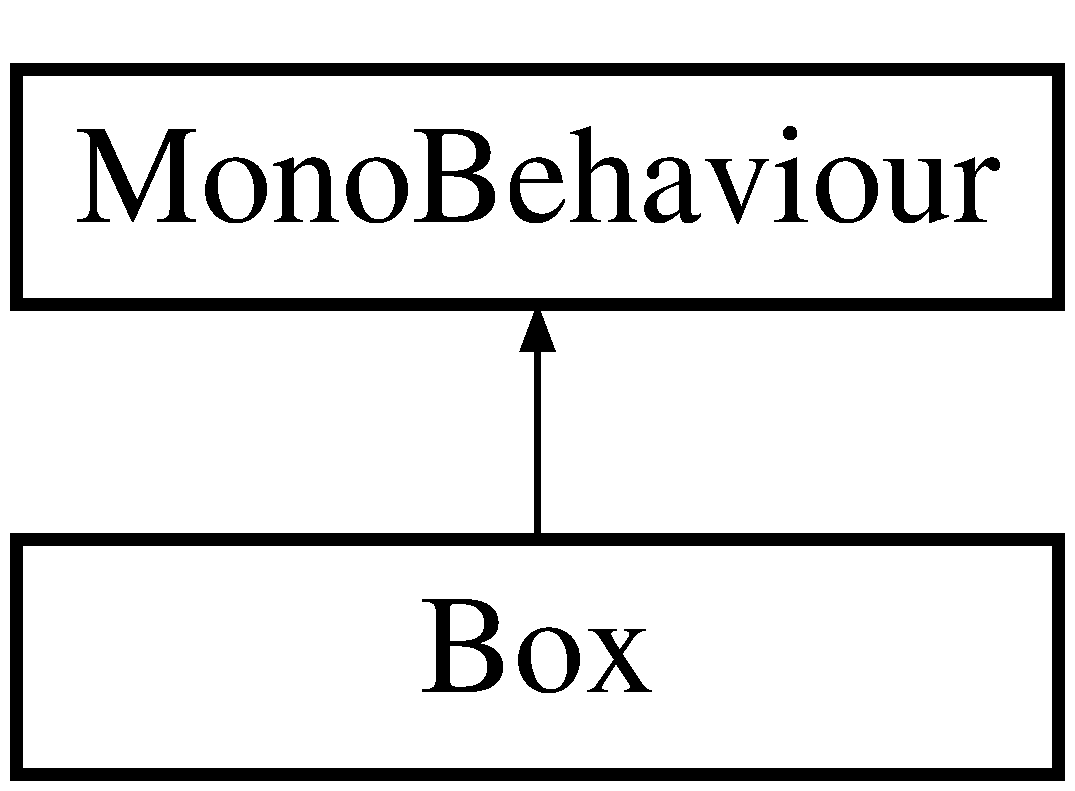
\includegraphics[height=2.000000cm]{class_box}
\end{center}
\end{figure}
\subsection*{Public Attributes}
\begin{DoxyCompactItemize}
\item 
Game\+Object \mbox{\hyperlink{class_box_ab1079b5543c8e8961ceb43899a5f850d}{new\+Instrument}}
\end{DoxyCompactItemize}


\subsection{Member Data Documentation}
\mbox{\Hypertarget{class_box_ab1079b5543c8e8961ceb43899a5f850d}\label{class_box_ab1079b5543c8e8961ceb43899a5f850d}} 
\index{Box@{Box}!new\+Instrument@{new\+Instrument}}
\index{new\+Instrument@{new\+Instrument}!Box@{Box}}
\subsubsection{\texorpdfstring{new\+Instrument}{newInstrument}}
{\footnotesize\ttfamily Game\+Object Box.\+new\+Instrument}



The documentation for this class was generated from the following file\+:\begin{DoxyCompactItemize}
\item 
Assets/\+Scripts/\+Objects/\mbox{\hyperlink{_box_8cs}{Box.\+cs}}\end{DoxyCompactItemize}

\hypertarget{class_box_shield}{}\section{Box\+Shield Class Reference}
\label{class_box_shield}\index{Box\+Shield@{Box\+Shield}}
Inheritance diagram for Box\+Shield\+:\begin{figure}[H]
\begin{center}
\leavevmode
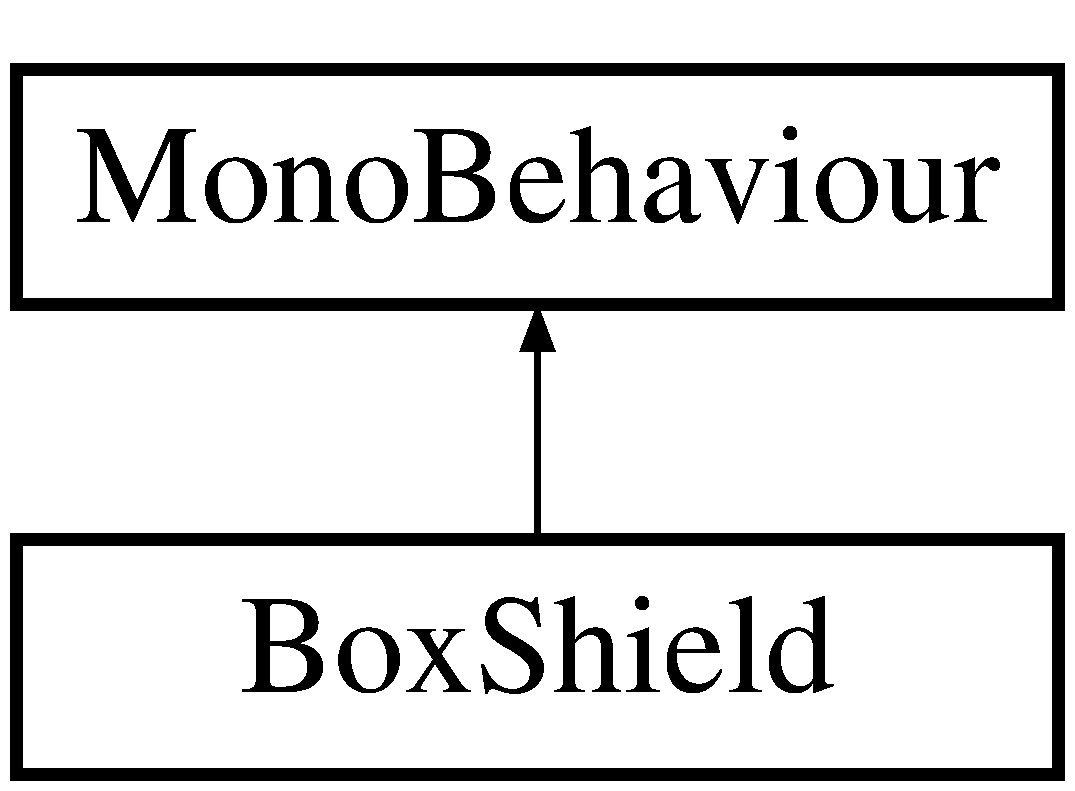
\includegraphics[height=2.000000cm]{class_box_shield}
\end{center}
\end{figure}


The documentation for this class was generated from the following file\+:\begin{DoxyCompactItemize}
\item 
Assets/\+Scripts/\+Objects/\mbox{\hyperlink{_box_shield_8cs}{Box\+Shield.\+cs}}\end{DoxyCompactItemize}

\hypertarget{class_bullet}{}\section{Bullet Class Reference}
\label{class_bullet}\index{Bullet@{Bullet}}
Inheritance diagram for Bullet\+:\begin{figure}[H]
\begin{center}
\leavevmode
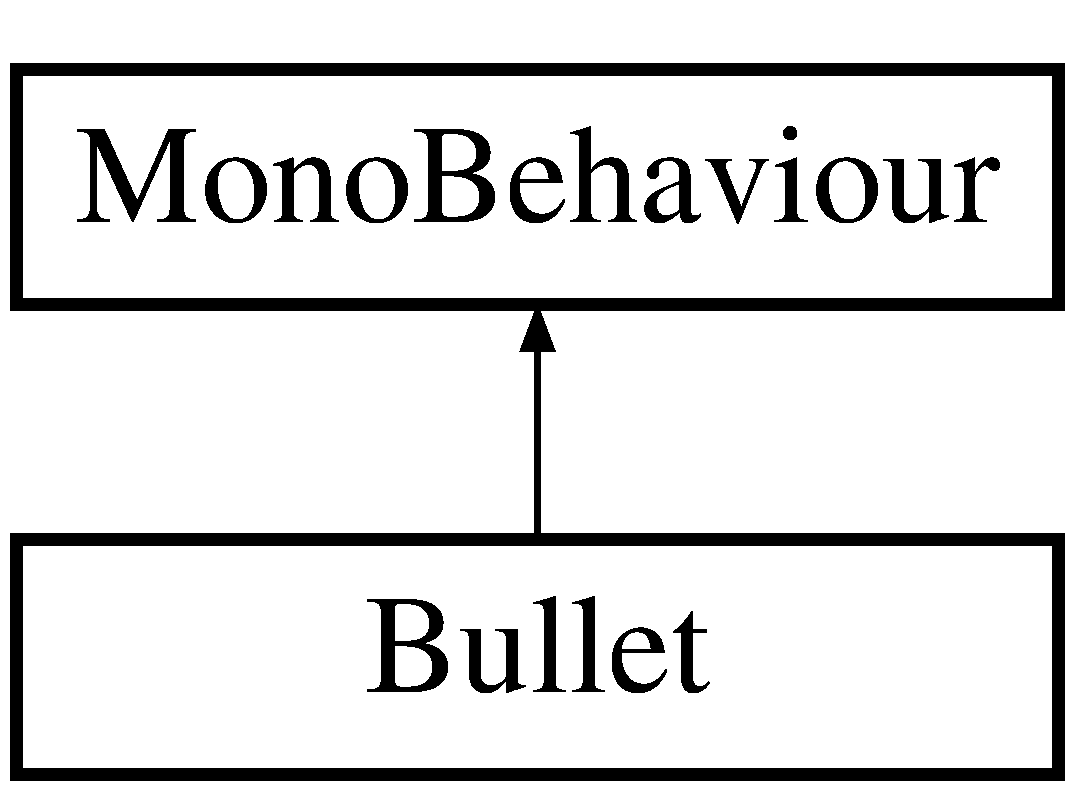
\includegraphics[height=2.000000cm]{class_bullet}
\end{center}
\end{figure}
\subsection*{Public Attributes}
\begin{DoxyCompactItemize}
\item 
Vector3 \mbox{\hyperlink{class_bullet_a3e2c779af8ba4b97394b3ae4be1404b5}{direction}}
\end{DoxyCompactItemize}
\subsection*{Properties}
\begin{DoxyCompactItemize}
\item 
Game\+Object \mbox{\hyperlink{class_bullet_ac42f67adee20458b6c1d1e3a50c37324}{Parent}}\hspace{0.3cm}{\ttfamily  \mbox{[}get, set\mbox{]}}
\item 
Vector3 \mbox{\hyperlink{class_bullet_a5c72494550e4c1b0afc815a3a10679d9}{Direction}}\hspace{0.3cm}{\ttfamily  \mbox{[}set\mbox{]}}
\item 
Color \mbox{\hyperlink{class_bullet_a11c93a49641814a887a9275cf5f927b2}{Color}}\hspace{0.3cm}{\ttfamily  \mbox{[}set\mbox{]}}
\end{DoxyCompactItemize}


\subsection{Member Data Documentation}
\mbox{\Hypertarget{class_bullet_a3e2c779af8ba4b97394b3ae4be1404b5}\label{class_bullet_a3e2c779af8ba4b97394b3ae4be1404b5}} 
\index{Bullet@{Bullet}!direction@{direction}}
\index{direction@{direction}!Bullet@{Bullet}}
\subsubsection{\texorpdfstring{direction}{direction}}
{\footnotesize\ttfamily Vector3 Bullet.\+direction}



\subsection{Property Documentation}
\mbox{\Hypertarget{class_bullet_a11c93a49641814a887a9275cf5f927b2}\label{class_bullet_a11c93a49641814a887a9275cf5f927b2}} 
\index{Bullet@{Bullet}!Color@{Color}}
\index{Color@{Color}!Bullet@{Bullet}}
\subsubsection{\texorpdfstring{Color}{Color}}
{\footnotesize\ttfamily Color Bullet.\+Color\hspace{0.3cm}{\ttfamily [set]}}

\mbox{\Hypertarget{class_bullet_a5c72494550e4c1b0afc815a3a10679d9}\label{class_bullet_a5c72494550e4c1b0afc815a3a10679d9}} 
\index{Bullet@{Bullet}!Direction@{Direction}}
\index{Direction@{Direction}!Bullet@{Bullet}}
\subsubsection{\texorpdfstring{Direction}{Direction}}
{\footnotesize\ttfamily Vector3 Bullet.\+Direction\hspace{0.3cm}{\ttfamily [set]}}

\mbox{\Hypertarget{class_bullet_ac42f67adee20458b6c1d1e3a50c37324}\label{class_bullet_ac42f67adee20458b6c1d1e3a50c37324}} 
\index{Bullet@{Bullet}!Parent@{Parent}}
\index{Parent@{Parent}!Bullet@{Bullet}}
\subsubsection{\texorpdfstring{Parent}{Parent}}
{\footnotesize\ttfamily Game\+Object Bullet.\+Parent\hspace{0.3cm}{\ttfamily [get]}, {\ttfamily [set]}}



The documentation for this class was generated from the following file\+:\begin{DoxyCompactItemize}
\item 
Assets/\+Scripts/\+Objects/\mbox{\hyperlink{_bullet_8cs}{Bullet.\+cs}}\end{DoxyCompactItemize}

\hypertarget{class_button_manager}{}\section{Button\+Manager Class Reference}
\label{class_button_manager}\index{Button\+Manager@{Button\+Manager}}
Inheritance diagram for Button\+Manager\+:\begin{figure}[H]
\begin{center}
\leavevmode
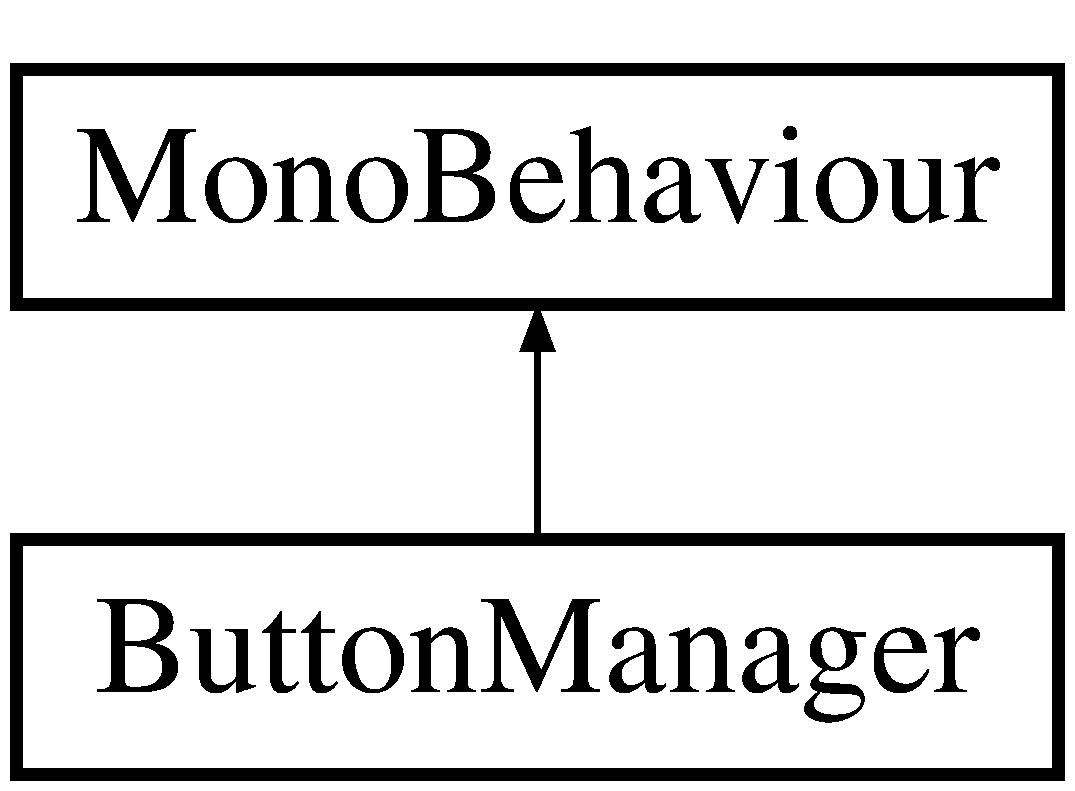
\includegraphics[height=2.000000cm]{class_button_manager}
\end{center}
\end{figure}
\subsection*{Public Member Functions}
\begin{DoxyCompactItemize}
\item 
void \mbox{\hyperlink{class_button_manager_a9728abfb3af4eb95eb03596fe831151b}{Play\+Game}} (Game\+Object obj)
\item 
void \mbox{\hyperlink{class_button_manager_a8984c32d0eb666371e65529605f3babf}{Exit\+Game}} ()
\end{DoxyCompactItemize}


\subsection{Member Function Documentation}
\mbox{\Hypertarget{class_button_manager_a8984c32d0eb666371e65529605f3babf}\label{class_button_manager_a8984c32d0eb666371e65529605f3babf}} 
\index{Button\+Manager@{Button\+Manager}!Exit\+Game@{Exit\+Game}}
\index{Exit\+Game@{Exit\+Game}!Button\+Manager@{Button\+Manager}}
\subsubsection{\texorpdfstring{Exit\+Game()}{ExitGame()}}
{\footnotesize\ttfamily void Button\+Manager.\+Exit\+Game (\begin{DoxyParamCaption}{ }\end{DoxyParamCaption})\hspace{0.3cm}{\ttfamily [inline]}}

\mbox{\Hypertarget{class_button_manager_a9728abfb3af4eb95eb03596fe831151b}\label{class_button_manager_a9728abfb3af4eb95eb03596fe831151b}} 
\index{Button\+Manager@{Button\+Manager}!Play\+Game@{Play\+Game}}
\index{Play\+Game@{Play\+Game}!Button\+Manager@{Button\+Manager}}
\subsubsection{\texorpdfstring{Play\+Game()}{PlayGame()}}
{\footnotesize\ttfamily void Button\+Manager.\+Play\+Game (\begin{DoxyParamCaption}\item[{Game\+Object}]{obj }\end{DoxyParamCaption})\hspace{0.3cm}{\ttfamily [inline]}}



The documentation for this class was generated from the following file\+:\begin{DoxyCompactItemize}
\item 
Assets/\+Scripts/\+Buttons/\mbox{\hyperlink{_button_manager_8cs}{Button\+Manager.\+cs}}\end{DoxyCompactItemize}

\hypertarget{class_camera_controller}{}\section{Camera\+Controller Class Reference}
\label{class_camera_controller}\index{Camera\+Controller@{Camera\+Controller}}
Inheritance diagram for Camera\+Controller\+:\begin{figure}[H]
\begin{center}
\leavevmode
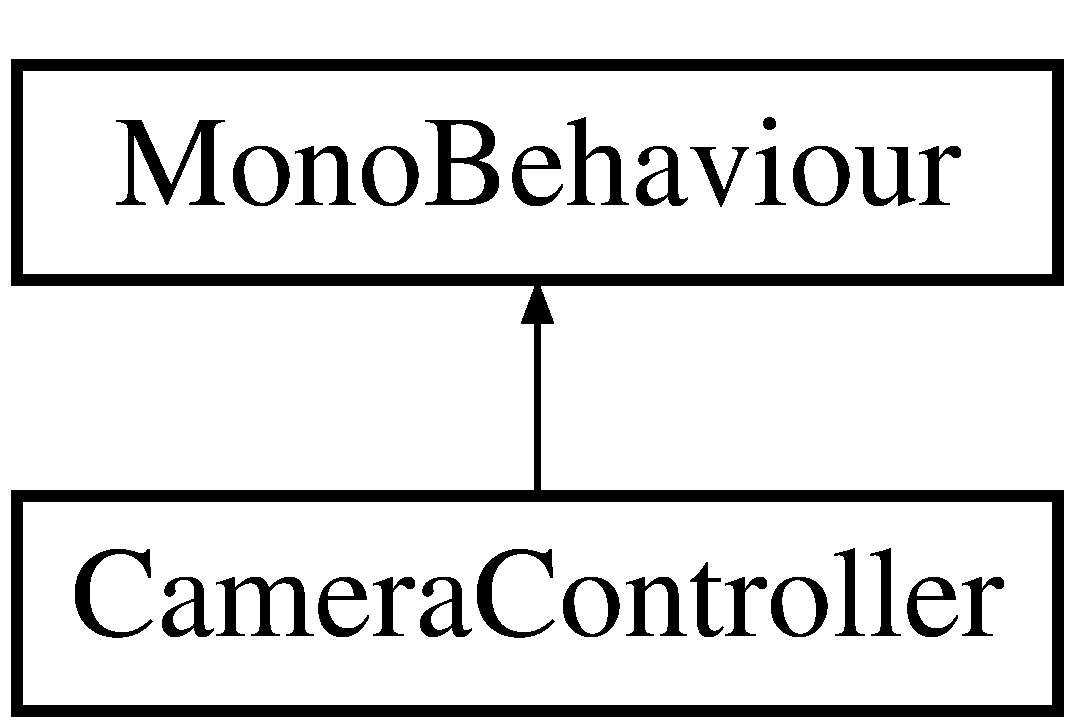
\includegraphics[height=2.000000cm]{class_camera_controller}
\end{center}
\end{figure}
\subsection*{Public Attributes}
\begin{DoxyCompactItemize}
\item 
bool \mbox{\hyperlink{class_camera_controller_a2ce0aa2f36420905ad36a7c4cdb65347}{find\+Player}} = true
\end{DoxyCompactItemize}


\subsection{Member Data Documentation}
\mbox{\Hypertarget{class_camera_controller_a2ce0aa2f36420905ad36a7c4cdb65347}\label{class_camera_controller_a2ce0aa2f36420905ad36a7c4cdb65347}} 
\index{Camera\+Controller@{Camera\+Controller}!find\+Player@{find\+Player}}
\index{find\+Player@{find\+Player}!Camera\+Controller@{Camera\+Controller}}
\subsubsection{\texorpdfstring{find\+Player}{findPlayer}}
{\footnotesize\ttfamily bool Camera\+Controller.\+find\+Player = true}



The documentation for this class was generated from the following file\+:\begin{DoxyCompactItemize}
\item 
Assets/\+Scripts/\+Camera/\mbox{\hyperlink{_camera_controller_8cs}{Camera\+Controller.\+cs}}\end{DoxyCompactItemize}

\hypertarget{class_camera_follow2_d}{}\section{Camera\+Follow2D Class Reference}
\label{class_camera_follow2_d}\index{Camera\+Follow2D@{Camera\+Follow2D}}
Inheritance diagram for Camera\+Follow2D\+:\begin{figure}[H]
\begin{center}
\leavevmode
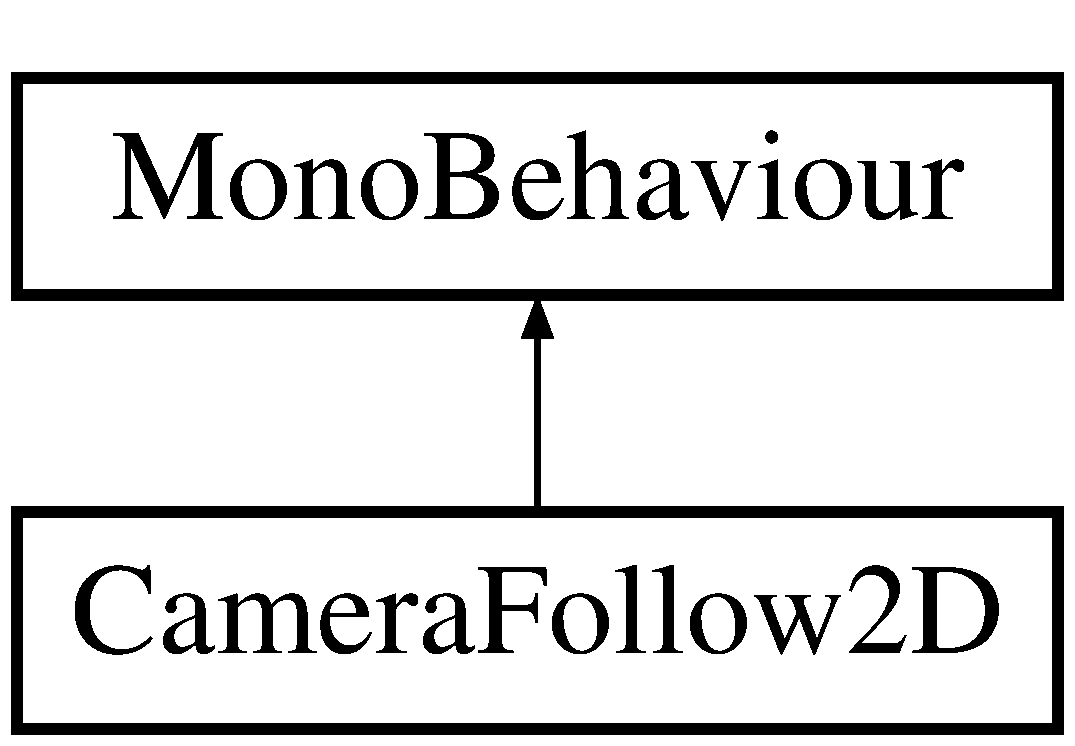
\includegraphics[height=2.000000cm]{class_camera_follow2_d}
\end{center}
\end{figure}
\subsection*{Public Member Functions}
\begin{DoxyCompactItemize}
\item 
void \mbox{\hyperlink{class_camera_follow2_d_a09ecf131b5803c849f033678a4f7074e}{Find\+Player}} (bool player\+Face\+Left)
\end{DoxyCompactItemize}
\subsection*{Public Attributes}
\begin{DoxyCompactItemize}
\item 
float \mbox{\hyperlink{class_camera_follow2_d_a37c1fc15ec814895aac4cfaef0112682}{damping}} = 1.\+5f
\item 
Vector2 \mbox{\hyperlink{class_camera_follow2_d_ad20b2de59ea17dac96326e9a1471564d}{offset}} = new Vector2(2f, 1f)
\item 
bool \mbox{\hyperlink{class_camera_follow2_d_ac2decd0164a2ea91bfc21fce22561c97}{face\+Left}}
\end{DoxyCompactItemize}


\subsection{Member Function Documentation}
\mbox{\Hypertarget{class_camera_follow2_d_a09ecf131b5803c849f033678a4f7074e}\label{class_camera_follow2_d_a09ecf131b5803c849f033678a4f7074e}} 
\index{Camera\+Follow2D@{Camera\+Follow2D}!Find\+Player@{Find\+Player}}
\index{Find\+Player@{Find\+Player}!Camera\+Follow2D@{Camera\+Follow2D}}
\subsubsection{\texorpdfstring{Find\+Player()}{FindPlayer()}}
{\footnotesize\ttfamily void Camera\+Follow2\+D.\+Find\+Player (\begin{DoxyParamCaption}\item[{bool}]{player\+Face\+Left }\end{DoxyParamCaption})\hspace{0.3cm}{\ttfamily [inline]}}



\subsection{Member Data Documentation}
\mbox{\Hypertarget{class_camera_follow2_d_a37c1fc15ec814895aac4cfaef0112682}\label{class_camera_follow2_d_a37c1fc15ec814895aac4cfaef0112682}} 
\index{Camera\+Follow2D@{Camera\+Follow2D}!damping@{damping}}
\index{damping@{damping}!Camera\+Follow2D@{Camera\+Follow2D}}
\subsubsection{\texorpdfstring{damping}{damping}}
{\footnotesize\ttfamily float Camera\+Follow2\+D.\+damping = 1.\+5f}

\mbox{\Hypertarget{class_camera_follow2_d_ac2decd0164a2ea91bfc21fce22561c97}\label{class_camera_follow2_d_ac2decd0164a2ea91bfc21fce22561c97}} 
\index{Camera\+Follow2D@{Camera\+Follow2D}!face\+Left@{face\+Left}}
\index{face\+Left@{face\+Left}!Camera\+Follow2D@{Camera\+Follow2D}}
\subsubsection{\texorpdfstring{face\+Left}{faceLeft}}
{\footnotesize\ttfamily bool Camera\+Follow2\+D.\+face\+Left}

\mbox{\Hypertarget{class_camera_follow2_d_ad20b2de59ea17dac96326e9a1471564d}\label{class_camera_follow2_d_ad20b2de59ea17dac96326e9a1471564d}} 
\index{Camera\+Follow2D@{Camera\+Follow2D}!offset@{offset}}
\index{offset@{offset}!Camera\+Follow2D@{Camera\+Follow2D}}
\subsubsection{\texorpdfstring{offset}{offset}}
{\footnotesize\ttfamily Vector2 Camera\+Follow2\+D.\+offset = new Vector2(2f, 1f)}



The documentation for this class was generated from the following file\+:\begin{DoxyCompactItemize}
\item 
Assets/\+Scripts/\+Camera/\mbox{\hyperlink{_camera_follow2_d_8cs}{Camera\+Follow2\+D.\+cs}}\end{DoxyCompactItemize}

\hypertarget{class_character}{}\section{Character Class Reference}
\label{class_character}\index{Character@{Character}}
Inheritance diagram for Character\+:\begin{figure}[H]
\begin{center}
\leavevmode
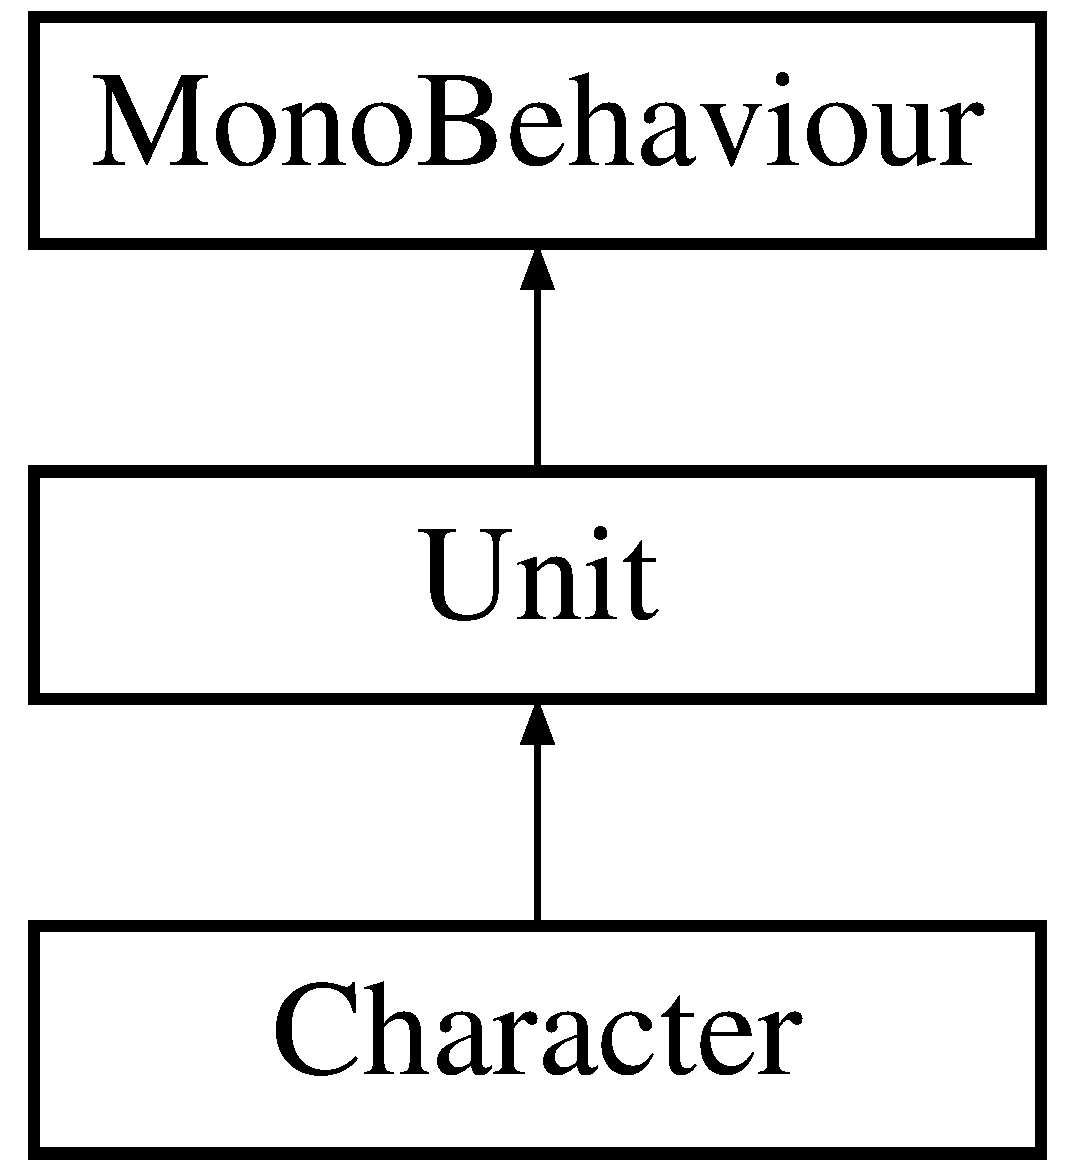
\includegraphics[height=3.000000cm]{class_character}
\end{center}
\end{figure}
\subsection*{Public Member Functions}
\begin{DoxyCompactItemize}
\item 
override void \mbox{\hyperlink{class_character_a4c92566bccf29f534c3863eb12fddba2}{Receive\+Damage}} ()
\end{DoxyCompactItemize}
\subsection*{Public Attributes}
\begin{DoxyCompactItemize}
\item 
bool \mbox{\hyperlink{class_character_ab0f4a965ac9a929654251db63b51131a}{can\+Make\+Magic}} = false
\item 
bool \mbox{\hyperlink{class_character_a07fd3e211945cdfc6d813127908d48fb}{can\+Be\+Protected}} = false
\item 
float \mbox{\hyperlink{class_character_a34ba4bab0f4e03bc819698826f483572}{speed}} = 3.\+0F
\end{DoxyCompactItemize}
\subsection*{Properties}
\begin{DoxyCompactItemize}
\item 
int \mbox{\hyperlink{class_character_a9aa02060768a4818a7be5439d4b2b34b}{Lives}}\hspace{0.3cm}{\ttfamily  \mbox{[}get, set\mbox{]}}
\end{DoxyCompactItemize}
\subsection*{Additional Inherited Members}


\subsection{Member Function Documentation}
\mbox{\Hypertarget{class_character_a4c92566bccf29f534c3863eb12fddba2}\label{class_character_a4c92566bccf29f534c3863eb12fddba2}} 
\index{Character@{Character}!Receive\+Damage@{Receive\+Damage}}
\index{Receive\+Damage@{Receive\+Damage}!Character@{Character}}
\subsubsection{\texorpdfstring{Receive\+Damage()}{ReceiveDamage()}}
{\footnotesize\ttfamily override void Character.\+Receive\+Damage (\begin{DoxyParamCaption}{ }\end{DoxyParamCaption})\hspace{0.3cm}{\ttfamily [inline]}, {\ttfamily [virtual]}}



Reimplemented from \mbox{\hyperlink{class_unit_a698a459fd5eeef7fc906f4657b723fa4}{Unit}}.



\subsection{Member Data Documentation}
\mbox{\Hypertarget{class_character_a07fd3e211945cdfc6d813127908d48fb}\label{class_character_a07fd3e211945cdfc6d813127908d48fb}} 
\index{Character@{Character}!can\+Be\+Protected@{can\+Be\+Protected}}
\index{can\+Be\+Protected@{can\+Be\+Protected}!Character@{Character}}
\subsubsection{\texorpdfstring{can\+Be\+Protected}{canBeProtected}}
{\footnotesize\ttfamily bool Character.\+can\+Be\+Protected = false}

\mbox{\Hypertarget{class_character_ab0f4a965ac9a929654251db63b51131a}\label{class_character_ab0f4a965ac9a929654251db63b51131a}} 
\index{Character@{Character}!can\+Make\+Magic@{can\+Make\+Magic}}
\index{can\+Make\+Magic@{can\+Make\+Magic}!Character@{Character}}
\subsubsection{\texorpdfstring{can\+Make\+Magic}{canMakeMagic}}
{\footnotesize\ttfamily bool Character.\+can\+Make\+Magic = false}

\mbox{\Hypertarget{class_character_a34ba4bab0f4e03bc819698826f483572}\label{class_character_a34ba4bab0f4e03bc819698826f483572}} 
\index{Character@{Character}!speed@{speed}}
\index{speed@{speed}!Character@{Character}}
\subsubsection{\texorpdfstring{speed}{speed}}
{\footnotesize\ttfamily float Character.\+speed = 3.\+0F}



\subsection{Property Documentation}
\mbox{\Hypertarget{class_character_a9aa02060768a4818a7be5439d4b2b34b}\label{class_character_a9aa02060768a4818a7be5439d4b2b34b}} 
\index{Character@{Character}!Lives@{Lives}}
\index{Lives@{Lives}!Character@{Character}}
\subsubsection{\texorpdfstring{Lives}{Lives}}
{\footnotesize\ttfamily int Character.\+Lives\hspace{0.3cm}{\ttfamily [get]}, {\ttfamily [set]}}



The documentation for this class was generated from the following file\+:\begin{DoxyCompactItemize}
\item 
Assets/\+Scripts/\mbox{\hyperlink{_character_8cs}{Character.\+cs}}\end{DoxyCompactItemize}

\hypertarget{class_chess_game_control}{}\section{Chess\+Game\+Control Class Reference}
\label{class_chess_game_control}\index{Chess\+Game\+Control@{Chess\+Game\+Control}}
Inheritance diagram for Chess\+Game\+Control\+:\begin{figure}[H]
\begin{center}
\leavevmode
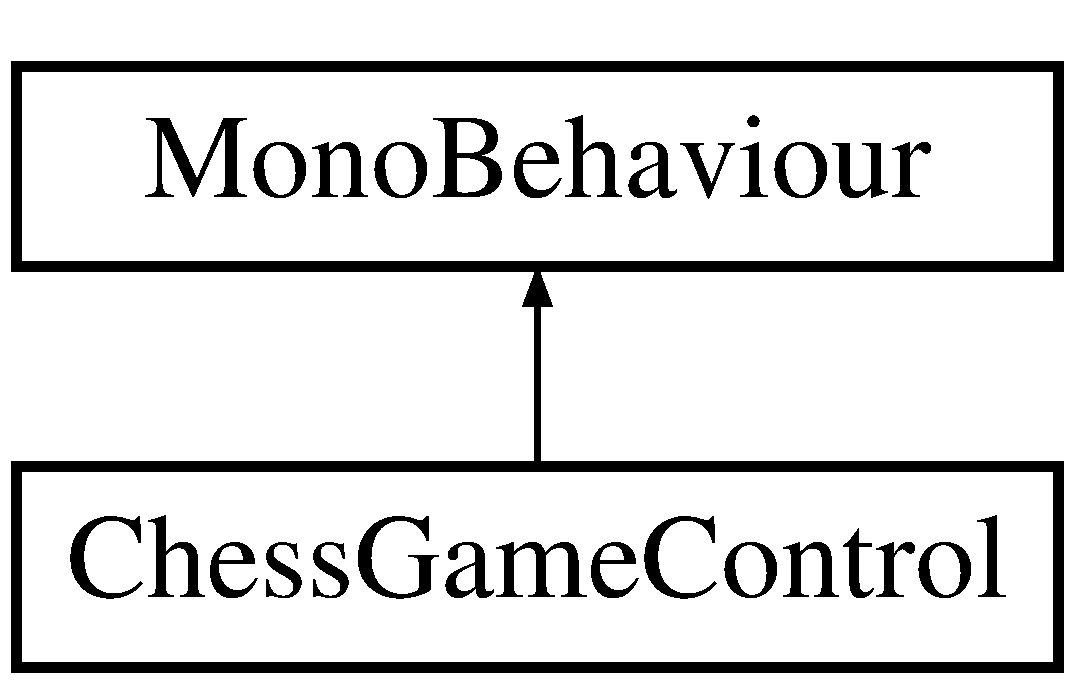
\includegraphics[height=2.000000cm]{class_chess_game_control}
\end{center}
\end{figure}
\subsection*{Public Member Functions}
\begin{DoxyCompactItemize}
\item 
void \mbox{\hyperlink{class_chess_game_control_affafb753ad71eda5251f7945674298d9}{Start\+New\+Game}} ()
\end{DoxyCompactItemize}
\subsection*{Static Public Member Functions}
\begin{DoxyCompactItemize}
\item 
static void \mbox{\hyperlink{class_chess_game_control_a3729a1181e9013740d165af9de103390}{Game\+Finish}} ()
\end{DoxyCompactItemize}
\subsection*{Public Attributes}
\begin{DoxyCompactItemize}
\item 
Game\+Object \mbox{[}$\,$\mbox{]} \mbox{\hyperlink{class_chess_game_control_afbb50d0fa87fbfd950b0c393f96b6bd5}{\+\_\+puzzle}}
\item 
float \mbox{\hyperlink{class_chess_game_control_a4418745fbd1dbff6ab10651da41f0fba}{start\+PosX}} = -\/6f
\item 
float \mbox{\hyperlink{class_chess_game_control_af53f18006dd9f5e14f84c8af7b8f18e6}{start\+PosY}} = 6f
\item 
float \mbox{\hyperlink{class_chess_game_control_a3415ff724cb50abbbc9a23336f6d2a93}{outX}} = 1.\+1f
\item 
float \mbox{\hyperlink{class_chess_game_control_a45bbddf6cacb5b0a01a2d938e7ad19b3}{outY}} = 1.\+1f
\item 
Text \mbox{\hyperlink{class_chess_game_control_afa13ec262edb1f71890c4b01898b9c19}{\+\_\+text}}
\end{DoxyCompactItemize}
\subsection*{Static Public Attributes}
\begin{DoxyCompactItemize}
\item 
static int \mbox{\hyperlink{class_chess_game_control_aac96797687bb522aa3aea376268775e8}{click}}
\item 
static Game\+Object \mbox{[},\mbox{]} \mbox{\hyperlink{class_chess_game_control_a7279acdb582d5633c8122b405293a059}{grid}}
\item 
static Vector3 \mbox{[},\mbox{]} \mbox{\hyperlink{class_chess_game_control_ada0f979d5d329c8280497c11c87e882a}{position}}
\item 
static bool \mbox{\hyperlink{class_chess_game_control_a50c474be4f430b946ca89f3e898a25a1}{win}}
\end{DoxyCompactItemize}


\subsection{Member Function Documentation}
\mbox{\Hypertarget{class_chess_game_control_a3729a1181e9013740d165af9de103390}\label{class_chess_game_control_a3729a1181e9013740d165af9de103390}} 
\index{Chess\+Game\+Control@{Chess\+Game\+Control}!Game\+Finish@{Game\+Finish}}
\index{Game\+Finish@{Game\+Finish}!Chess\+Game\+Control@{Chess\+Game\+Control}}
\subsubsection{\texorpdfstring{Game\+Finish()}{GameFinish()}}
{\footnotesize\ttfamily static void Chess\+Game\+Control.\+Game\+Finish (\begin{DoxyParamCaption}{ }\end{DoxyParamCaption})\hspace{0.3cm}{\ttfamily [inline]}, {\ttfamily [static]}}

\mbox{\Hypertarget{class_chess_game_control_affafb753ad71eda5251f7945674298d9}\label{class_chess_game_control_affafb753ad71eda5251f7945674298d9}} 
\index{Chess\+Game\+Control@{Chess\+Game\+Control}!Start\+New\+Game@{Start\+New\+Game}}
\index{Start\+New\+Game@{Start\+New\+Game}!Chess\+Game\+Control@{Chess\+Game\+Control}}
\subsubsection{\texorpdfstring{Start\+New\+Game()}{StartNewGame()}}
{\footnotesize\ttfamily void Chess\+Game\+Control.\+Start\+New\+Game (\begin{DoxyParamCaption}{ }\end{DoxyParamCaption})\hspace{0.3cm}{\ttfamily [inline]}}



\subsection{Member Data Documentation}
\mbox{\Hypertarget{class_chess_game_control_afbb50d0fa87fbfd950b0c393f96b6bd5}\label{class_chess_game_control_afbb50d0fa87fbfd950b0c393f96b6bd5}} 
\index{Chess\+Game\+Control@{Chess\+Game\+Control}!\+\_\+puzzle@{\+\_\+puzzle}}
\index{\+\_\+puzzle@{\+\_\+puzzle}!Chess\+Game\+Control@{Chess\+Game\+Control}}
\subsubsection{\texorpdfstring{\+\_\+puzzle}{\_puzzle}}
{\footnotesize\ttfamily Game\+Object \mbox{[}$\,$\mbox{]} Chess\+Game\+Control.\+\_\+puzzle}

\mbox{\Hypertarget{class_chess_game_control_afa13ec262edb1f71890c4b01898b9c19}\label{class_chess_game_control_afa13ec262edb1f71890c4b01898b9c19}} 
\index{Chess\+Game\+Control@{Chess\+Game\+Control}!\+\_\+text@{\+\_\+text}}
\index{\+\_\+text@{\+\_\+text}!Chess\+Game\+Control@{Chess\+Game\+Control}}
\subsubsection{\texorpdfstring{\+\_\+text}{\_text}}
{\footnotesize\ttfamily Text Chess\+Game\+Control.\+\_\+text}

\mbox{\Hypertarget{class_chess_game_control_aac96797687bb522aa3aea376268775e8}\label{class_chess_game_control_aac96797687bb522aa3aea376268775e8}} 
\index{Chess\+Game\+Control@{Chess\+Game\+Control}!click@{click}}
\index{click@{click}!Chess\+Game\+Control@{Chess\+Game\+Control}}
\subsubsection{\texorpdfstring{click}{click}}
{\footnotesize\ttfamily int Chess\+Game\+Control.\+click\hspace{0.3cm}{\ttfamily [static]}}

\mbox{\Hypertarget{class_chess_game_control_a7279acdb582d5633c8122b405293a059}\label{class_chess_game_control_a7279acdb582d5633c8122b405293a059}} 
\index{Chess\+Game\+Control@{Chess\+Game\+Control}!grid@{grid}}
\index{grid@{grid}!Chess\+Game\+Control@{Chess\+Game\+Control}}
\subsubsection{\texorpdfstring{grid}{grid}}
{\footnotesize\ttfamily Game\+Object \mbox{[},\mbox{]} Chess\+Game\+Control.\+grid\hspace{0.3cm}{\ttfamily [static]}}

\mbox{\Hypertarget{class_chess_game_control_a3415ff724cb50abbbc9a23336f6d2a93}\label{class_chess_game_control_a3415ff724cb50abbbc9a23336f6d2a93}} 
\index{Chess\+Game\+Control@{Chess\+Game\+Control}!outX@{outX}}
\index{outX@{outX}!Chess\+Game\+Control@{Chess\+Game\+Control}}
\subsubsection{\texorpdfstring{outX}{outX}}
{\footnotesize\ttfamily float Chess\+Game\+Control.\+outX = 1.\+1f}

\mbox{\Hypertarget{class_chess_game_control_a45bbddf6cacb5b0a01a2d938e7ad19b3}\label{class_chess_game_control_a45bbddf6cacb5b0a01a2d938e7ad19b3}} 
\index{Chess\+Game\+Control@{Chess\+Game\+Control}!outY@{outY}}
\index{outY@{outY}!Chess\+Game\+Control@{Chess\+Game\+Control}}
\subsubsection{\texorpdfstring{outY}{outY}}
{\footnotesize\ttfamily float Chess\+Game\+Control.\+outY = 1.\+1f}

\mbox{\Hypertarget{class_chess_game_control_ada0f979d5d329c8280497c11c87e882a}\label{class_chess_game_control_ada0f979d5d329c8280497c11c87e882a}} 
\index{Chess\+Game\+Control@{Chess\+Game\+Control}!position@{position}}
\index{position@{position}!Chess\+Game\+Control@{Chess\+Game\+Control}}
\subsubsection{\texorpdfstring{position}{position}}
{\footnotesize\ttfamily Vector3 \mbox{[},\mbox{]} Chess\+Game\+Control.\+position\hspace{0.3cm}{\ttfamily [static]}}

\mbox{\Hypertarget{class_chess_game_control_a4418745fbd1dbff6ab10651da41f0fba}\label{class_chess_game_control_a4418745fbd1dbff6ab10651da41f0fba}} 
\index{Chess\+Game\+Control@{Chess\+Game\+Control}!start\+PosX@{start\+PosX}}
\index{start\+PosX@{start\+PosX}!Chess\+Game\+Control@{Chess\+Game\+Control}}
\subsubsection{\texorpdfstring{start\+PosX}{startPosX}}
{\footnotesize\ttfamily float Chess\+Game\+Control.\+start\+PosX = -\/6f}

\mbox{\Hypertarget{class_chess_game_control_af53f18006dd9f5e14f84c8af7b8f18e6}\label{class_chess_game_control_af53f18006dd9f5e14f84c8af7b8f18e6}} 
\index{Chess\+Game\+Control@{Chess\+Game\+Control}!start\+PosY@{start\+PosY}}
\index{start\+PosY@{start\+PosY}!Chess\+Game\+Control@{Chess\+Game\+Control}}
\subsubsection{\texorpdfstring{start\+PosY}{startPosY}}
{\footnotesize\ttfamily float Chess\+Game\+Control.\+start\+PosY = 6f}

\mbox{\Hypertarget{class_chess_game_control_a50c474be4f430b946ca89f3e898a25a1}\label{class_chess_game_control_a50c474be4f430b946ca89f3e898a25a1}} 
\index{Chess\+Game\+Control@{Chess\+Game\+Control}!win@{win}}
\index{win@{win}!Chess\+Game\+Control@{Chess\+Game\+Control}}
\subsubsection{\texorpdfstring{win}{win}}
{\footnotesize\ttfamily bool Chess\+Game\+Control.\+win\hspace{0.3cm}{\ttfamily [static]}}



The documentation for this class was generated from the following file\+:\begin{DoxyCompactItemize}
\item 
Assets/\+Scripts/\+Chess\+Game/\mbox{\hyperlink{_chess_game_control_8cs}{Chess\+Game\+Control.\+cs}}\end{DoxyCompactItemize}

\hypertarget{class_demon}{}\section{Demon Class Reference}
\label{class_demon}\index{Demon@{Demon}}
Inheritance diagram for Demon\+:\begin{figure}[H]
\begin{center}
\leavevmode
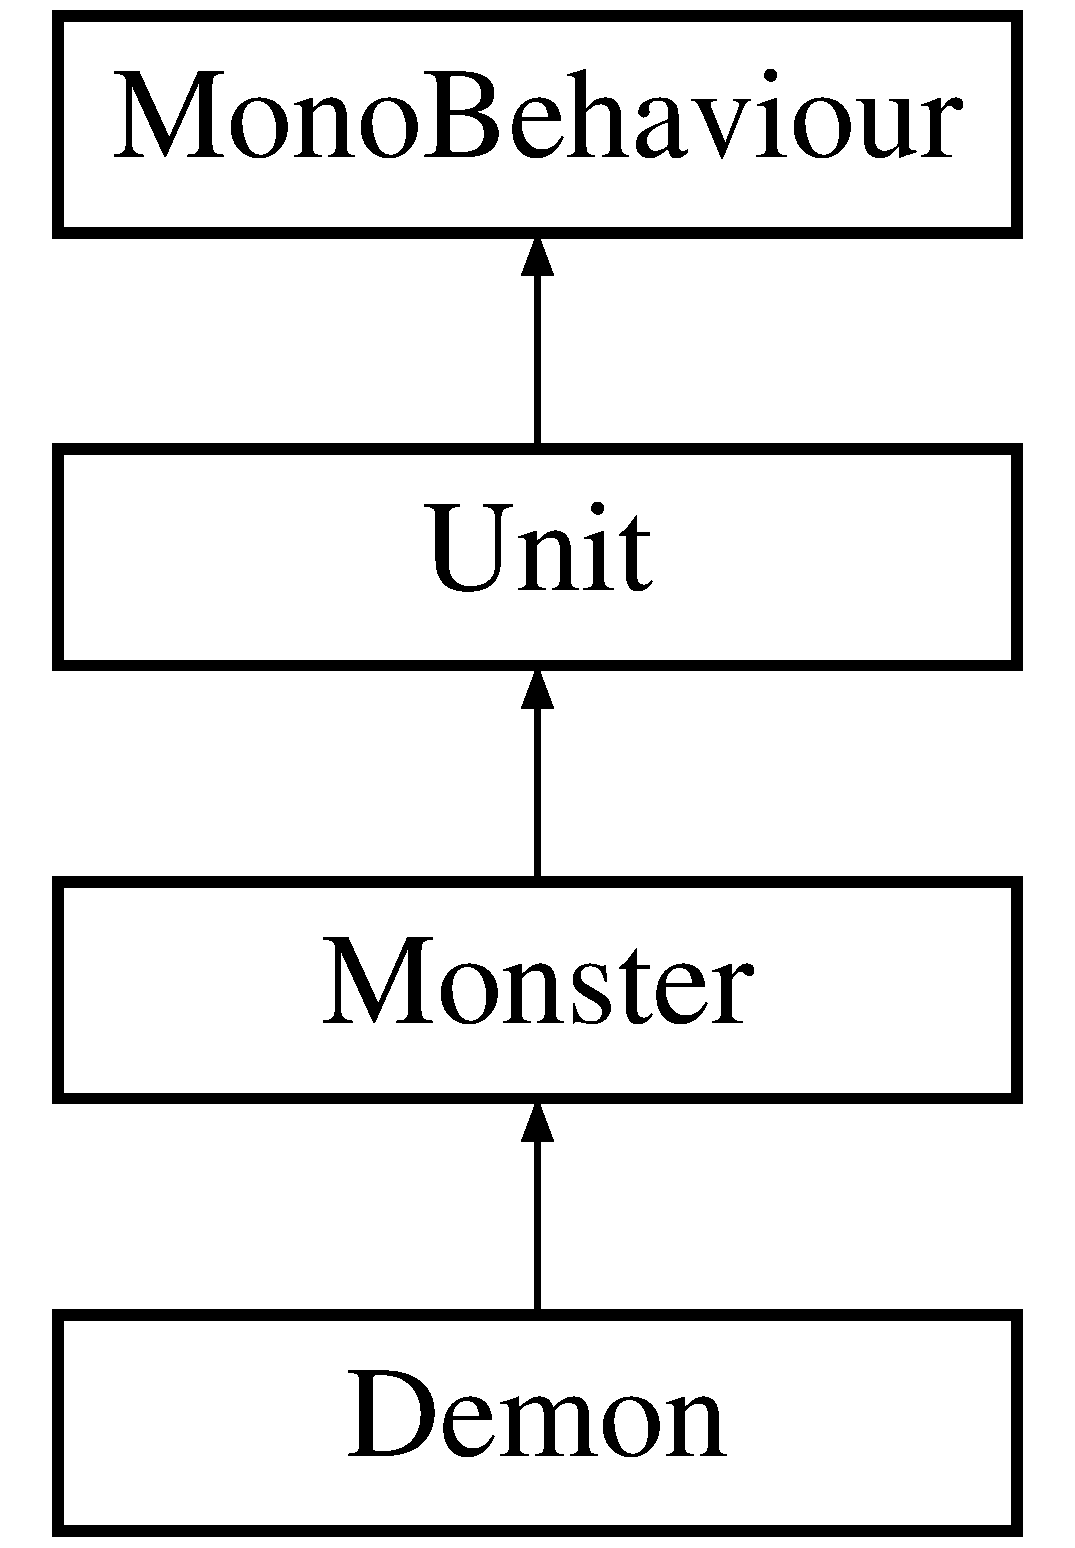
\includegraphics[height=4.000000cm]{class_demon}
\end{center}
\end{figure}
\subsection*{Public Member Functions}
\begin{DoxyCompactItemize}
\item 
override void \mbox{\hyperlink{class_demon_a90dc4738a3cab182e3daa2da35cbbbc6}{Receive\+Damage}} ()
\end{DoxyCompactItemize}
\subsection*{Public Attributes}
\begin{DoxyCompactItemize}
\item 
float \mbox{\hyperlink{class_demon_aa70173ebd268fdf60a979f64d3c8a2aa}{speed}} = 7.\+0F
\end{DoxyCompactItemize}
\subsection*{Static Public Attributes}
\begin{DoxyCompactItemize}
\item 
static bool \mbox{\hyperlink{class_demon_a89b29e16599d3d03485366ac8f29678d}{one\+Thread}} = false
\end{DoxyCompactItemize}
\subsection*{Protected Member Functions}
\begin{DoxyCompactItemize}
\item 
override void \mbox{\hyperlink{class_demon_a1a87c40897c33f1a752e66807fb53f34}{Awake}} ()
\item 
override void \mbox{\hyperlink{class_demon_ae40d3b2d791569cd6517117aa19335b3}{Start}} ()
\item 
override void \mbox{\hyperlink{class_demon_aa0c85beffd46a97daa76e65bb2388444}{On\+Trigger\+Enter2D}} (Collider2D collider)
\end{DoxyCompactItemize}


\subsection{Member Function Documentation}
\mbox{\Hypertarget{class_demon_a1a87c40897c33f1a752e66807fb53f34}\label{class_demon_a1a87c40897c33f1a752e66807fb53f34}} 
\index{Demon@{Demon}!Awake@{Awake}}
\index{Awake@{Awake}!Demon@{Demon}}
\subsubsection{\texorpdfstring{Awake()}{Awake()}}
{\footnotesize\ttfamily override void Demon.\+Awake (\begin{DoxyParamCaption}{ }\end{DoxyParamCaption})\hspace{0.3cm}{\ttfamily [inline]}, {\ttfamily [protected]}, {\ttfamily [virtual]}}



Reimplemented from \mbox{\hyperlink{class_monster_a3ccbdc33e8e7e6fb20286338ad17c6f2}{Monster}}.

\mbox{\Hypertarget{class_demon_aa0c85beffd46a97daa76e65bb2388444}\label{class_demon_aa0c85beffd46a97daa76e65bb2388444}} 
\index{Demon@{Demon}!On\+Trigger\+Enter2D@{On\+Trigger\+Enter2D}}
\index{On\+Trigger\+Enter2D@{On\+Trigger\+Enter2D}!Demon@{Demon}}
\subsubsection{\texorpdfstring{On\+Trigger\+Enter2\+D()}{OnTriggerEnter2D()}}
{\footnotesize\ttfamily override void Demon.\+On\+Trigger\+Enter2D (\begin{DoxyParamCaption}\item[{Collider2D}]{collider }\end{DoxyParamCaption})\hspace{0.3cm}{\ttfamily [inline]}, {\ttfamily [protected]}, {\ttfamily [virtual]}}



Reimplemented from \mbox{\hyperlink{class_monster_af6ac6a4c01088e6b4abf79da772cecff}{Monster}}.

\mbox{\Hypertarget{class_demon_a90dc4738a3cab182e3daa2da35cbbbc6}\label{class_demon_a90dc4738a3cab182e3daa2da35cbbbc6}} 
\index{Demon@{Demon}!Receive\+Damage@{Receive\+Damage}}
\index{Receive\+Damage@{Receive\+Damage}!Demon@{Demon}}
\subsubsection{\texorpdfstring{Receive\+Damage()}{ReceiveDamage()}}
{\footnotesize\ttfamily override void Demon.\+Receive\+Damage (\begin{DoxyParamCaption}{ }\end{DoxyParamCaption})\hspace{0.3cm}{\ttfamily [inline]}, {\ttfamily [virtual]}}



Reimplemented from \mbox{\hyperlink{class_unit_a698a459fd5eeef7fc906f4657b723fa4}{Unit}}.

\mbox{\Hypertarget{class_demon_ae40d3b2d791569cd6517117aa19335b3}\label{class_demon_ae40d3b2d791569cd6517117aa19335b3}} 
\index{Demon@{Demon}!Start@{Start}}
\index{Start@{Start}!Demon@{Demon}}
\subsubsection{\texorpdfstring{Start()}{Start()}}
{\footnotesize\ttfamily override void Demon.\+Start (\begin{DoxyParamCaption}{ }\end{DoxyParamCaption})\hspace{0.3cm}{\ttfamily [inline]}, {\ttfamily [protected]}, {\ttfamily [virtual]}}



Reimplemented from \mbox{\hyperlink{class_monster_a79f369a560bdcf5b3dfaf8c9382582d8}{Monster}}.



\subsection{Member Data Documentation}
\mbox{\Hypertarget{class_demon_a89b29e16599d3d03485366ac8f29678d}\label{class_demon_a89b29e16599d3d03485366ac8f29678d}} 
\index{Demon@{Demon}!one\+Thread@{one\+Thread}}
\index{one\+Thread@{one\+Thread}!Demon@{Demon}}
\subsubsection{\texorpdfstring{one\+Thread}{oneThread}}
{\footnotesize\ttfamily bool Demon.\+one\+Thread = false\hspace{0.3cm}{\ttfamily [static]}}

\mbox{\Hypertarget{class_demon_aa70173ebd268fdf60a979f64d3c8a2aa}\label{class_demon_aa70173ebd268fdf60a979f64d3c8a2aa}} 
\index{Demon@{Demon}!speed@{speed}}
\index{speed@{speed}!Demon@{Demon}}
\subsubsection{\texorpdfstring{speed}{speed}}
{\footnotesize\ttfamily float Demon.\+speed = 7.\+0F}



The documentation for this class was generated from the following file\+:\begin{DoxyCompactItemize}
\item 
Assets/\+Scripts/\mbox{\hyperlink{_demon_8cs}{Demon.\+cs}}\end{DoxyCompactItemize}

\hypertarget{class_door_trigger}{}\section{Door\+Trigger Class Reference}
\label{class_door_trigger}\index{Door\+Trigger@{Door\+Trigger}}
Inheritance diagram for Door\+Trigger\+:\begin{figure}[H]
\begin{center}
\leavevmode
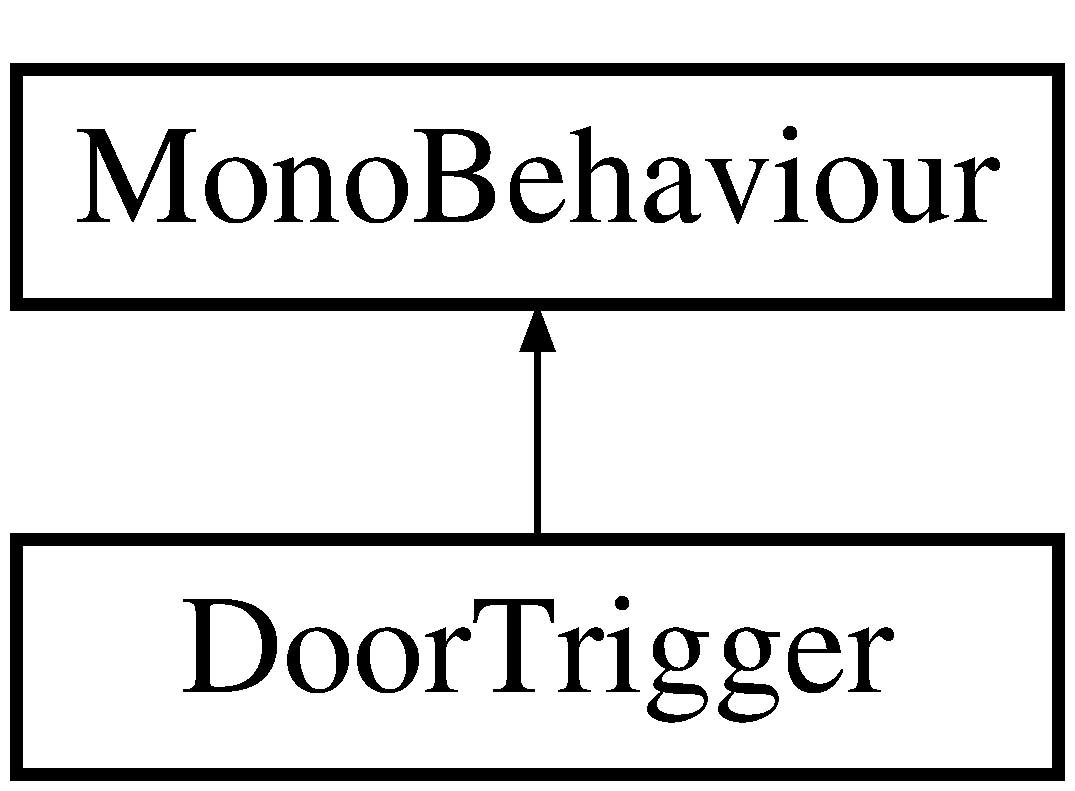
\includegraphics[height=2.000000cm]{class_door_trigger}
\end{center}
\end{figure}


The documentation for this class was generated from the following file\+:\begin{DoxyCompactItemize}
\item 
Assets/\+Scripts/\+Objects/\mbox{\hyperlink{_door_trigger_8cs}{Door\+Trigger.\+cs}}\end{DoxyCompactItemize}

\hypertarget{classempty}{}\section{empty Class Reference}
\label{classempty}\index{empty@{empty}}
Inheritance diagram for empty\+:\begin{figure}[H]
\begin{center}
\leavevmode
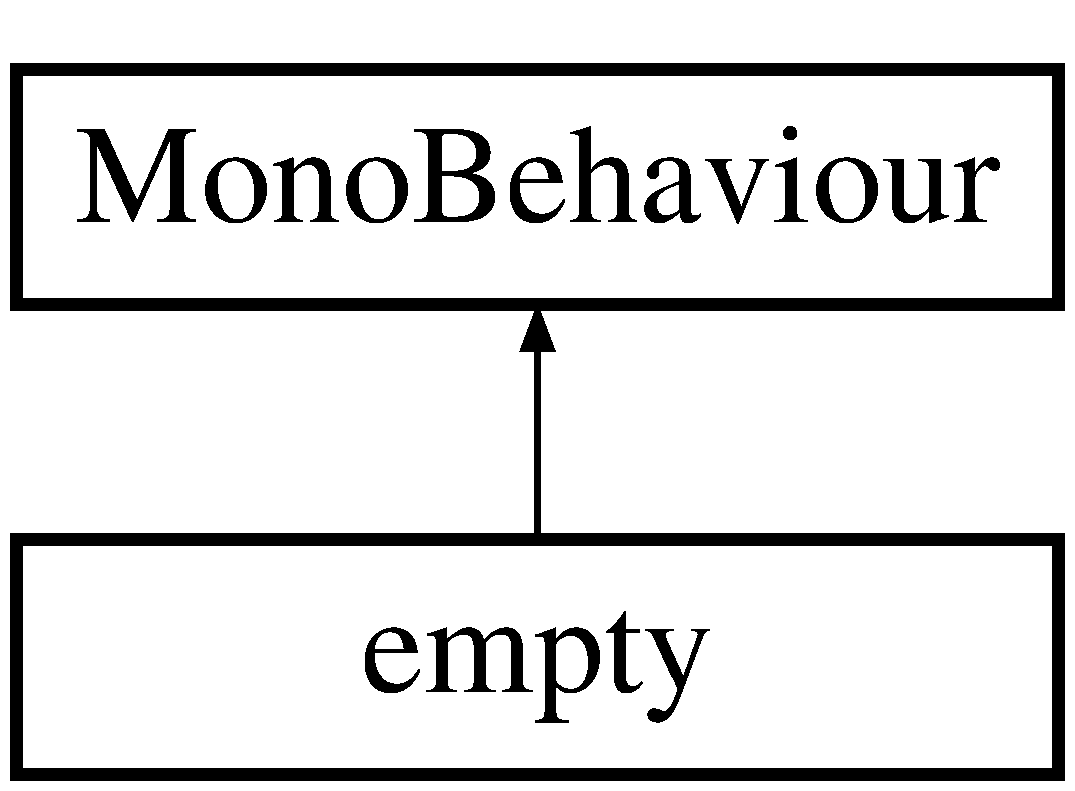
\includegraphics[height=2.000000cm]{classempty}
\end{center}
\end{figure}


The documentation for this class was generated from the following file\+:\begin{DoxyCompactItemize}
\item 
Assets/\+Scripts/\mbox{\hyperlink{empty_8cs}{empty.\+cs}}\end{DoxyCompactItemize}

\hypertarget{classfly_platform}{}\section{fly\+Platform Class Reference}
\label{classfly_platform}\index{fly\+Platform@{fly\+Platform}}
Inheritance diagram for fly\+Platform\+:\begin{figure}[H]
\begin{center}
\leavevmode
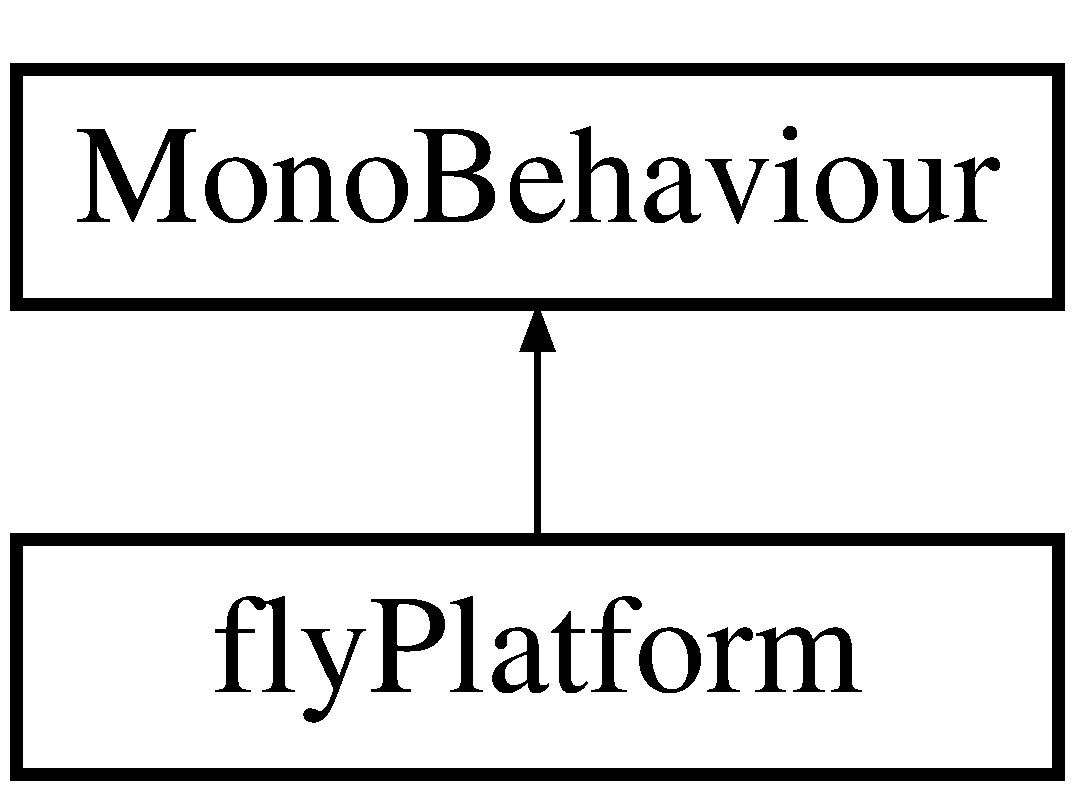
\includegraphics[height=2.000000cm]{classfly_platform}
\end{center}
\end{figure}
\subsection*{Public Attributes}
\begin{DoxyCompactItemize}
\item 
bool \mbox{\hyperlink{classfly_platform_acbbfd6480b1b6f5c169136478b63f217}{i}}
\item 
Transform \mbox{\hyperlink{classfly_platform_ada60b6e640fea01d20ead9c900dd42db}{target1}}
\item 
Transform \mbox{\hyperlink{classfly_platform_a6d9c0311b4c421ba400f7fbf34deeec2}{target2}}
\item 
float \mbox{\hyperlink{classfly_platform_aa1ce895856228c9e3c84f1f0410022de}{speed}} = 4.\+0F
\end{DoxyCompactItemize}


\subsection{Member Data Documentation}
\mbox{\Hypertarget{classfly_platform_acbbfd6480b1b6f5c169136478b63f217}\label{classfly_platform_acbbfd6480b1b6f5c169136478b63f217}} 
\index{fly\+Platform@{fly\+Platform}!i@{i}}
\index{i@{i}!fly\+Platform@{fly\+Platform}}
\subsubsection{\texorpdfstring{i}{i}}
{\footnotesize\ttfamily bool fly\+Platform.\+i}

\mbox{\Hypertarget{classfly_platform_aa1ce895856228c9e3c84f1f0410022de}\label{classfly_platform_aa1ce895856228c9e3c84f1f0410022de}} 
\index{fly\+Platform@{fly\+Platform}!speed@{speed}}
\index{speed@{speed}!fly\+Platform@{fly\+Platform}}
\subsubsection{\texorpdfstring{speed}{speed}}
{\footnotesize\ttfamily float fly\+Platform.\+speed = 4.\+0F}

\mbox{\Hypertarget{classfly_platform_ada60b6e640fea01d20ead9c900dd42db}\label{classfly_platform_ada60b6e640fea01d20ead9c900dd42db}} 
\index{fly\+Platform@{fly\+Platform}!target1@{target1}}
\index{target1@{target1}!fly\+Platform@{fly\+Platform}}
\subsubsection{\texorpdfstring{target1}{target1}}
{\footnotesize\ttfamily Transform fly\+Platform.\+target1}

\mbox{\Hypertarget{classfly_platform_a6d9c0311b4c421ba400f7fbf34deeec2}\label{classfly_platform_a6d9c0311b4c421ba400f7fbf34deeec2}} 
\index{fly\+Platform@{fly\+Platform}!target2@{target2}}
\index{target2@{target2}!fly\+Platform@{fly\+Platform}}
\subsubsection{\texorpdfstring{target2}{target2}}
{\footnotesize\ttfamily Transform fly\+Platform.\+target2}



The documentation for this class was generated from the following file\+:\begin{DoxyCompactItemize}
\item 
Assets/\+Scripts/\+Objects/\mbox{\hyperlink{fly_platform_8cs}{fly\+Platform.\+cs}}\end{DoxyCompactItemize}

\hypertarget{classfly_up}{}\section{fly\+Up Class Reference}
\label{classfly_up}\index{fly\+Up@{fly\+Up}}
Inheritance diagram for fly\+Up\+:\begin{figure}[H]
\begin{center}
\leavevmode
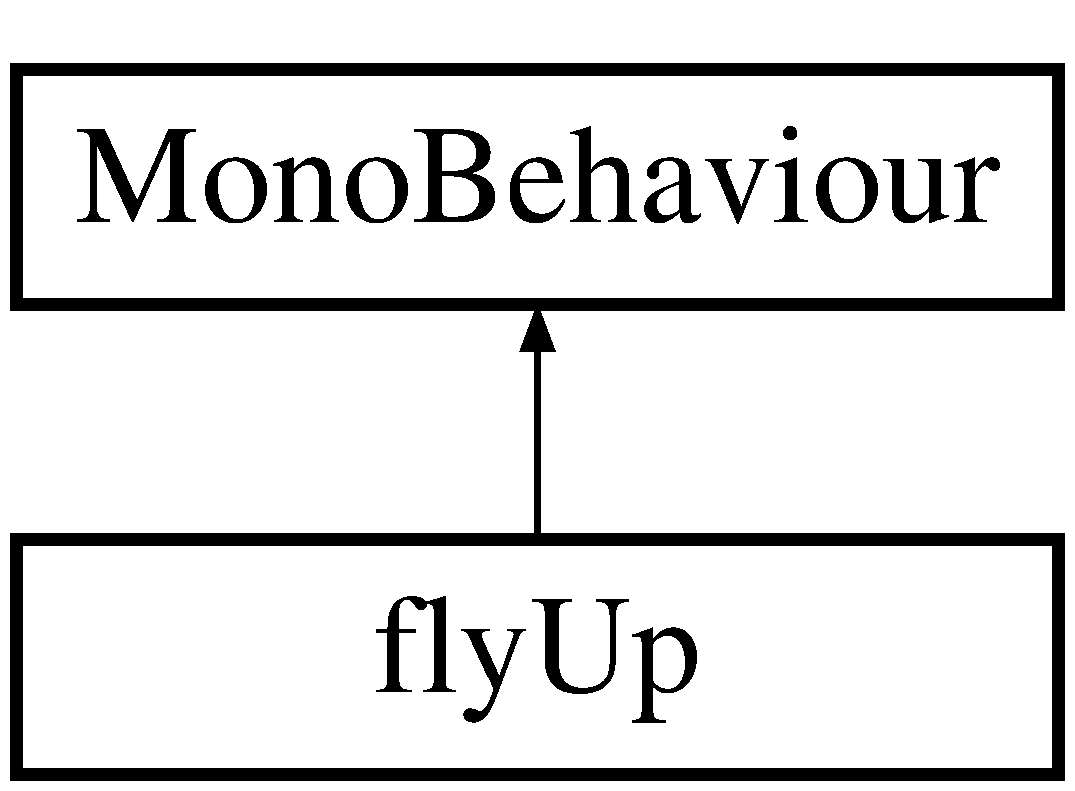
\includegraphics[height=2.000000cm]{classfly_up}
\end{center}
\end{figure}


The documentation for this class was generated from the following file\+:\begin{DoxyCompactItemize}
\item 
Assets/\+Scripts/\mbox{\hyperlink{fly_up_8cs}{fly\+Up.\+cs}}\end{DoxyCompactItemize}

\hypertarget{class_heart}{}\section{Heart Class Reference}
\label{class_heart}\index{Heart@{Heart}}
Inheritance diagram for Heart\+:\begin{figure}[H]
\begin{center}
\leavevmode
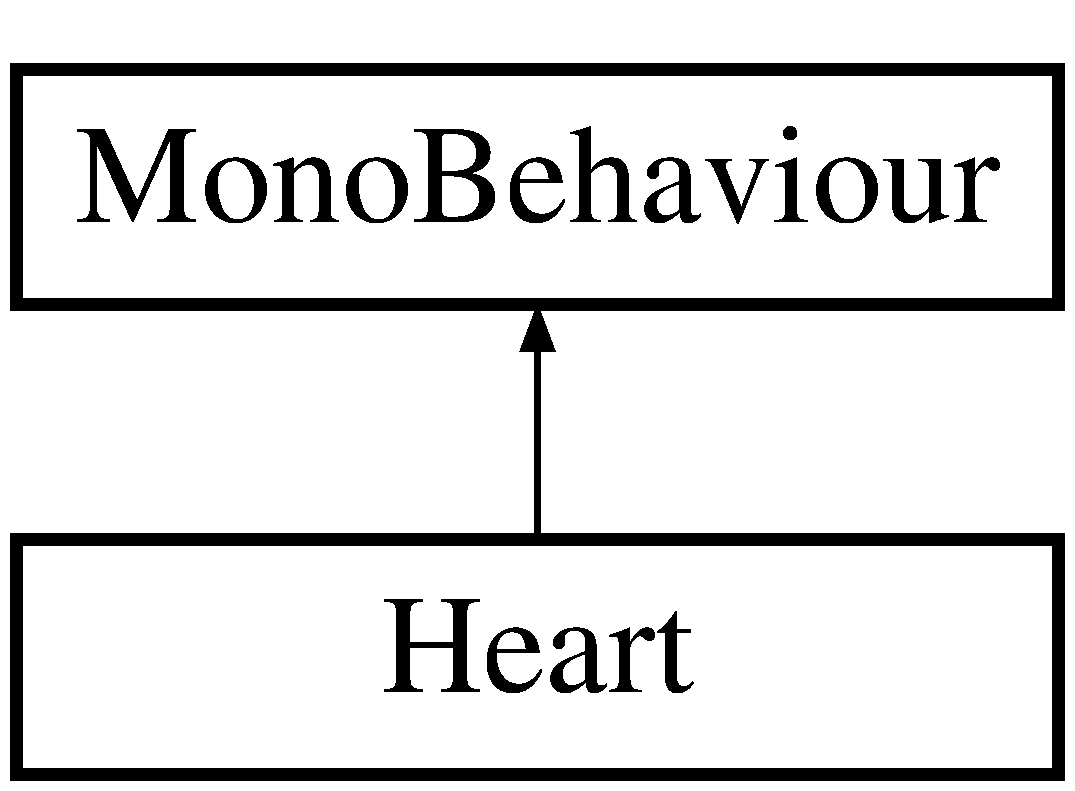
\includegraphics[height=2.000000cm]{class_heart}
\end{center}
\end{figure}


The documentation for this class was generated from the following file\+:\begin{DoxyCompactItemize}
\item 
Assets/\+Scripts/\+Objects/\mbox{\hyperlink{_heart_8cs}{Heart.\+cs}}\end{DoxyCompactItemize}

\hypertarget{class_ice_platform}{}\section{Ice\+Platform Class Reference}
\label{class_ice_platform}\index{Ice\+Platform@{Ice\+Platform}}
Inheritance diagram for Ice\+Platform\+:\begin{figure}[H]
\begin{center}
\leavevmode
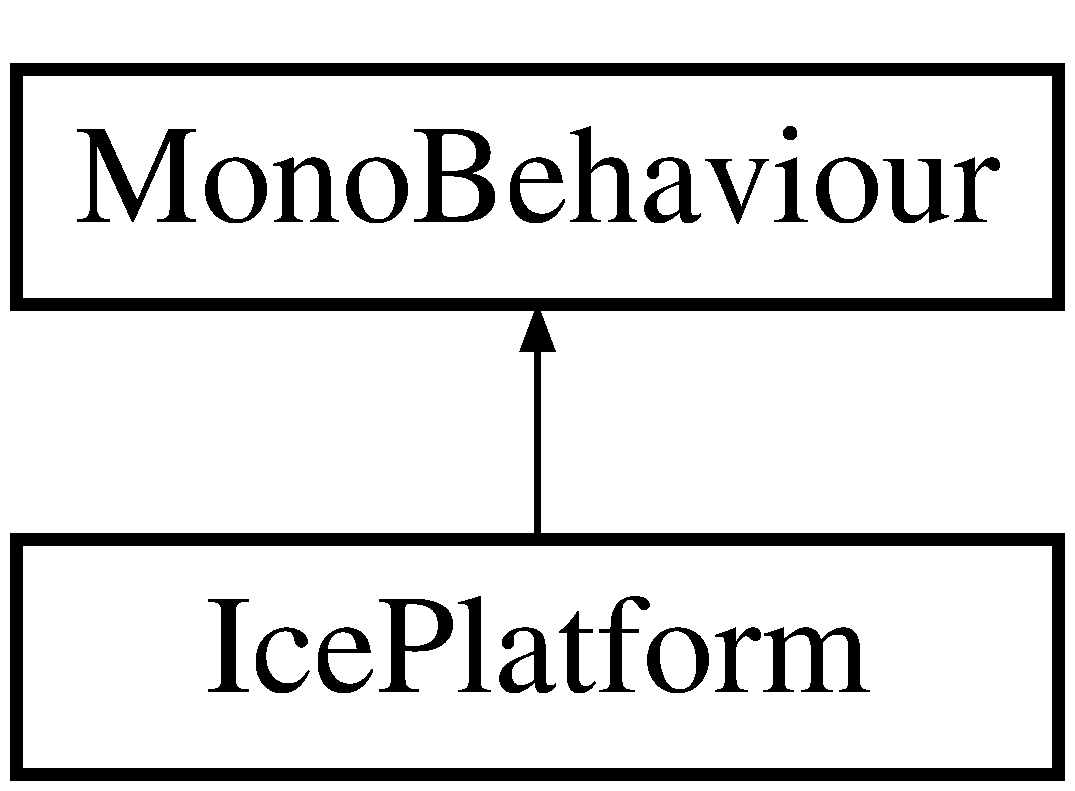
\includegraphics[height=2.000000cm]{class_ice_platform}
\end{center}
\end{figure}
\subsection*{Public Attributes}
\begin{DoxyCompactItemize}
\item 
float \mbox{\hyperlink{class_ice_platform_ac049bab48bb4d34f1a3c6858cfc138d4}{acceleration}} = 1.\+0F
\end{DoxyCompactItemize}


\subsection{Member Data Documentation}
\mbox{\Hypertarget{class_ice_platform_ac049bab48bb4d34f1a3c6858cfc138d4}\label{class_ice_platform_ac049bab48bb4d34f1a3c6858cfc138d4}} 
\index{Ice\+Platform@{Ice\+Platform}!acceleration@{acceleration}}
\index{acceleration@{acceleration}!Ice\+Platform@{Ice\+Platform}}
\subsubsection{\texorpdfstring{acceleration}{acceleration}}
{\footnotesize\ttfamily float Ice\+Platform.\+acceleration = 1.\+0F}



The documentation for this class was generated from the following file\+:\begin{DoxyCompactItemize}
\item 
Assets/\+Scripts/\+Objects/\mbox{\hyperlink{_ice_platform_8cs}{Ice\+Platform.\+cs}}\end{DoxyCompactItemize}

\hypertarget{class_lever1}{}\section{Lever1 Class Reference}
\label{class_lever1}\index{Lever1@{Lever1}}
Inheritance diagram for Lever1\+:\begin{figure}[H]
\begin{center}
\leavevmode
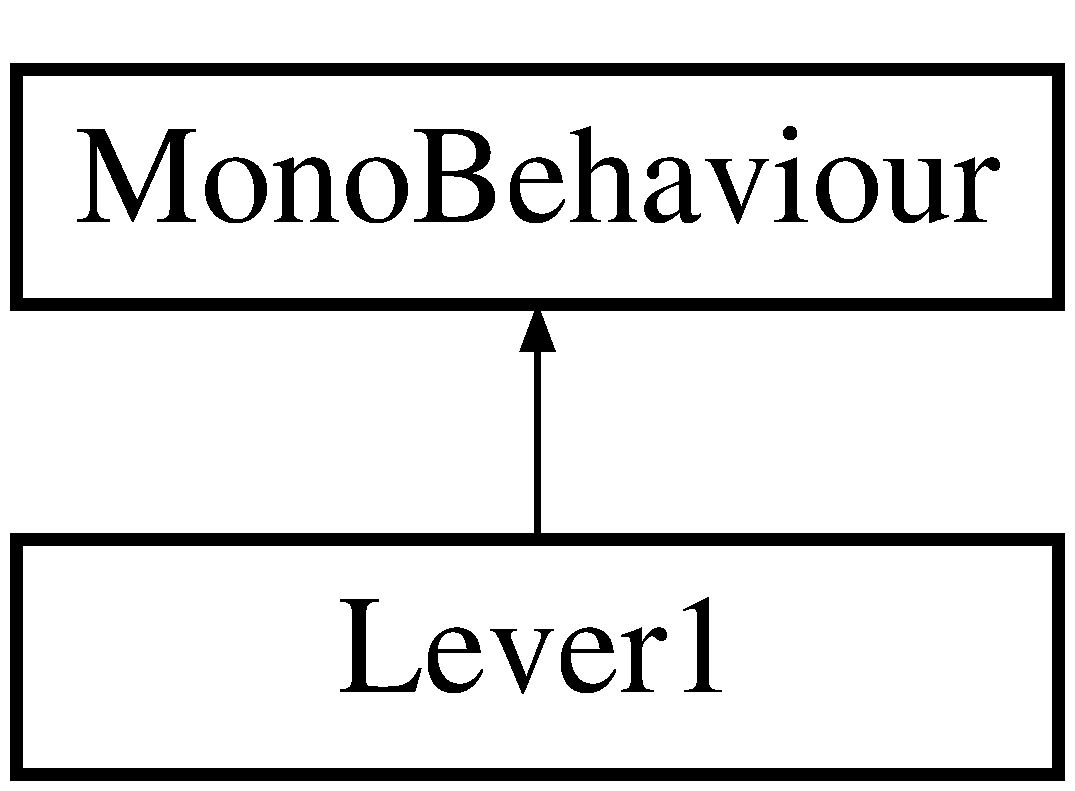
\includegraphics[height=2.000000cm]{class_lever1}
\end{center}
\end{figure}
\subsection*{Public Attributes}
\begin{DoxyCompactItemize}
\item 
bool \mbox{\hyperlink{class_lever1_abb6ee7bf7584e20bf3d576797a441257}{fly\+Platform}} = false
\end{DoxyCompactItemize}


\subsection{Member Data Documentation}
\mbox{\Hypertarget{class_lever1_abb6ee7bf7584e20bf3d576797a441257}\label{class_lever1_abb6ee7bf7584e20bf3d576797a441257}} 
\index{Lever1@{Lever1}!fly\+Platform@{fly\+Platform}}
\index{fly\+Platform@{fly\+Platform}!Lever1@{Lever1}}
\subsubsection{\texorpdfstring{fly\+Platform}{flyPlatform}}
{\footnotesize\ttfamily bool Lever1.\+fly\+Platform = false}



The documentation for this class was generated from the following file\+:\begin{DoxyCompactItemize}
\item 
Assets/\+Scripts/\+Objects/\mbox{\hyperlink{_lever1_8cs}{Lever1.\+cs}}\end{DoxyCompactItemize}

\hypertarget{class_lives_bar}{}\section{Lives\+Bar Class Reference}
\label{class_lives_bar}\index{Lives\+Bar@{Lives\+Bar}}
Inheritance diagram for Lives\+Bar\+:\begin{figure}[H]
\begin{center}
\leavevmode
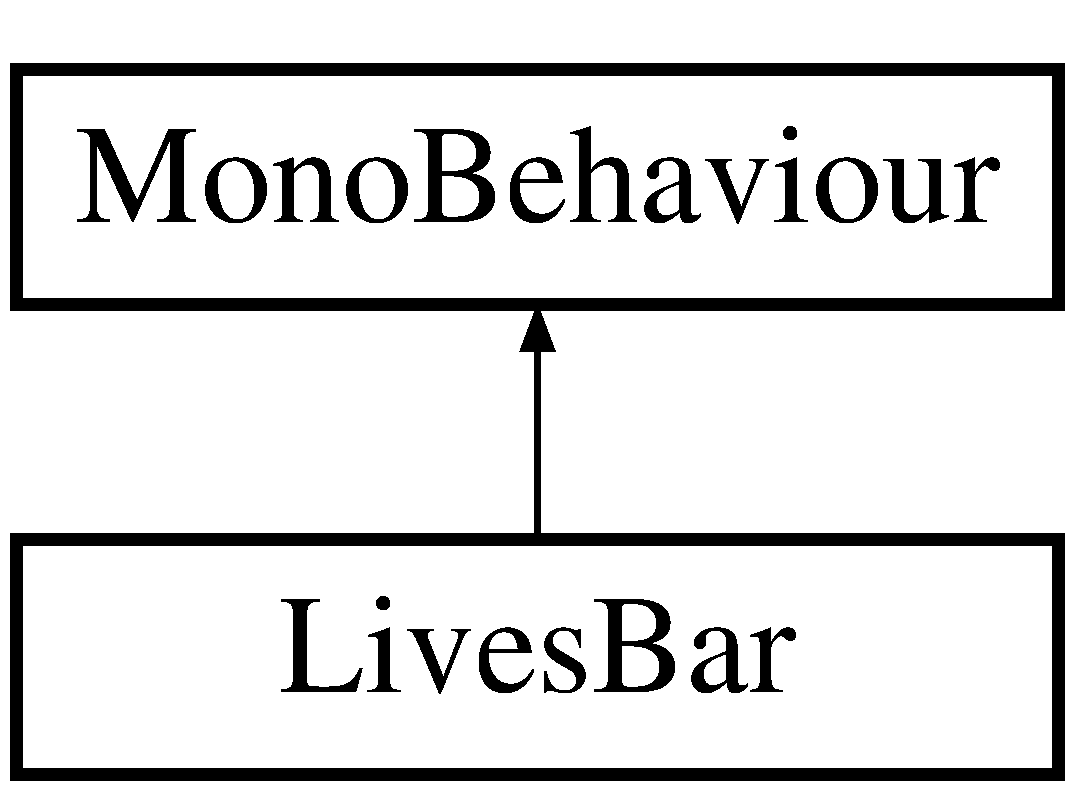
\includegraphics[height=2.000000cm]{class_lives_bar}
\end{center}
\end{figure}
\subsection*{Public Member Functions}
\begin{DoxyCompactItemize}
\item 
void \mbox{\hyperlink{class_lives_bar_a5fa833098a1cba59edab020f51e69795}{Refresh}} ()
\end{DoxyCompactItemize}


\subsection{Member Function Documentation}
\mbox{\Hypertarget{class_lives_bar_a5fa833098a1cba59edab020f51e69795}\label{class_lives_bar_a5fa833098a1cba59edab020f51e69795}} 
\index{Lives\+Bar@{Lives\+Bar}!Refresh@{Refresh}}
\index{Refresh@{Refresh}!Lives\+Bar@{Lives\+Bar}}
\subsubsection{\texorpdfstring{Refresh()}{Refresh()}}
{\footnotesize\ttfamily void Lives\+Bar.\+Refresh (\begin{DoxyParamCaption}{ }\end{DoxyParamCaption})\hspace{0.3cm}{\ttfamily [inline]}}



The documentation for this class was generated from the following file\+:\begin{DoxyCompactItemize}
\item 
Assets/\+Scripts/\+Objects/\mbox{\hyperlink{_lives_bar_8cs}{Lives\+Bar.\+cs}}\end{DoxyCompactItemize}

\hypertarget{class_monster}{}\section{Monster Class Reference}
\label{class_monster}\index{Monster@{Monster}}
Inheritance diagram for Monster\+:\begin{figure}[H]
\begin{center}
\leavevmode
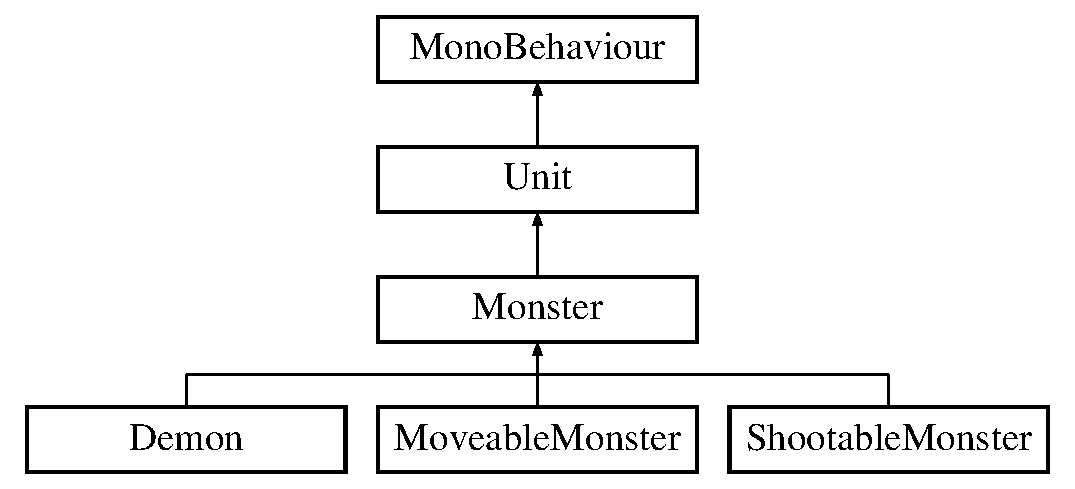
\includegraphics[height=4.000000cm]{class_monster}
\end{center}
\end{figure}
\subsection*{Protected Member Functions}
\begin{DoxyCompactItemize}
\item 
virtual void \mbox{\hyperlink{class_monster_a3ccbdc33e8e7e6fb20286338ad17c6f2}{Awake}} ()
\item 
virtual void \mbox{\hyperlink{class_monster_a79f369a560bdcf5b3dfaf8c9382582d8}{Start}} ()
\item 
virtual void \mbox{\hyperlink{class_monster_a91c04bb8ad53b26283de5f5bab20b789}{Update}} ()
\item 
virtual void \mbox{\hyperlink{class_monster_af6ac6a4c01088e6b4abf79da772cecff}{On\+Trigger\+Enter2D}} (Collider2D collider)
\end{DoxyCompactItemize}
\subsection*{Additional Inherited Members}


\subsection{Member Function Documentation}
\mbox{\Hypertarget{class_monster_a3ccbdc33e8e7e6fb20286338ad17c6f2}\label{class_monster_a3ccbdc33e8e7e6fb20286338ad17c6f2}} 
\index{Monster@{Monster}!Awake@{Awake}}
\index{Awake@{Awake}!Monster@{Monster}}
\subsubsection{\texorpdfstring{Awake()}{Awake()}}
{\footnotesize\ttfamily virtual void Monster.\+Awake (\begin{DoxyParamCaption}{ }\end{DoxyParamCaption})\hspace{0.3cm}{\ttfamily [inline]}, {\ttfamily [protected]}, {\ttfamily [virtual]}}



Reimplemented in \mbox{\hyperlink{class_demon_a1a87c40897c33f1a752e66807fb53f34}{Demon}}, \mbox{\hyperlink{class_shootable_monster_adfb9638b7a397563df4ab94c2db20ec0}{Shootable\+Monster}}, and \mbox{\hyperlink{class_moveable_monster_ae4e3c98d944fa303cf1b2c7f4a05a342}{Moveable\+Monster}}.

\mbox{\Hypertarget{class_monster_af6ac6a4c01088e6b4abf79da772cecff}\label{class_monster_af6ac6a4c01088e6b4abf79da772cecff}} 
\index{Monster@{Monster}!On\+Trigger\+Enter2D@{On\+Trigger\+Enter2D}}
\index{On\+Trigger\+Enter2D@{On\+Trigger\+Enter2D}!Monster@{Monster}}
\subsubsection{\texorpdfstring{On\+Trigger\+Enter2\+D()}{OnTriggerEnter2D()}}
{\footnotesize\ttfamily virtual void Monster.\+On\+Trigger\+Enter2D (\begin{DoxyParamCaption}\item[{Collider2D}]{collider }\end{DoxyParamCaption})\hspace{0.3cm}{\ttfamily [inline]}, {\ttfamily [protected]}, {\ttfamily [virtual]}}



Reimplemented in \mbox{\hyperlink{class_demon_aa0c85beffd46a97daa76e65bb2388444}{Demon}}, \mbox{\hyperlink{class_shootable_monster_a6c350a976d1bb37db2c663834c90e83b}{Shootable\+Monster}}, and \mbox{\hyperlink{class_moveable_monster_a07aefb0242f24f5b0f2b4cd820b31522}{Moveable\+Monster}}.

\mbox{\Hypertarget{class_monster_a79f369a560bdcf5b3dfaf8c9382582d8}\label{class_monster_a79f369a560bdcf5b3dfaf8c9382582d8}} 
\index{Monster@{Monster}!Start@{Start}}
\index{Start@{Start}!Monster@{Monster}}
\subsubsection{\texorpdfstring{Start()}{Start()}}
{\footnotesize\ttfamily virtual void Monster.\+Start (\begin{DoxyParamCaption}{ }\end{DoxyParamCaption})\hspace{0.3cm}{\ttfamily [inline]}, {\ttfamily [protected]}, {\ttfamily [virtual]}}



Reimplemented in \mbox{\hyperlink{class_demon_ae40d3b2d791569cd6517117aa19335b3}{Demon}}, \mbox{\hyperlink{class_shootable_monster_a0e26de95298ec75a591ecede3c1d8cb9}{Shootable\+Monster}}, and \mbox{\hyperlink{class_moveable_monster_a898a6098d4dd0226084e36f3a1c7f093}{Moveable\+Monster}}.

\mbox{\Hypertarget{class_monster_a91c04bb8ad53b26283de5f5bab20b789}\label{class_monster_a91c04bb8ad53b26283de5f5bab20b789}} 
\index{Monster@{Monster}!Update@{Update}}
\index{Update@{Update}!Monster@{Monster}}
\subsubsection{\texorpdfstring{Update()}{Update()}}
{\footnotesize\ttfamily virtual void Monster.\+Update (\begin{DoxyParamCaption}{ }\end{DoxyParamCaption})\hspace{0.3cm}{\ttfamily [inline]}, {\ttfamily [protected]}, {\ttfamily [virtual]}}



Reimplemented in \mbox{\hyperlink{class_moveable_monster_a03035ace68ce00f475ba1ef194ef5595}{Moveable\+Monster}}.



The documentation for this class was generated from the following file\+:\begin{DoxyCompactItemize}
\item 
Assets/\+Scripts/\+Monsters/\mbox{\hyperlink{_monster_8cs}{Monster.\+cs}}\end{DoxyCompactItemize}

\hypertarget{class_moveable_monster}{}\section{Moveable\+Monster Class Reference}
\label{class_moveable_monster}\index{Moveable\+Monster@{Moveable\+Monster}}
Inheritance diagram for Moveable\+Monster\+:\begin{figure}[H]
\begin{center}
\leavevmode
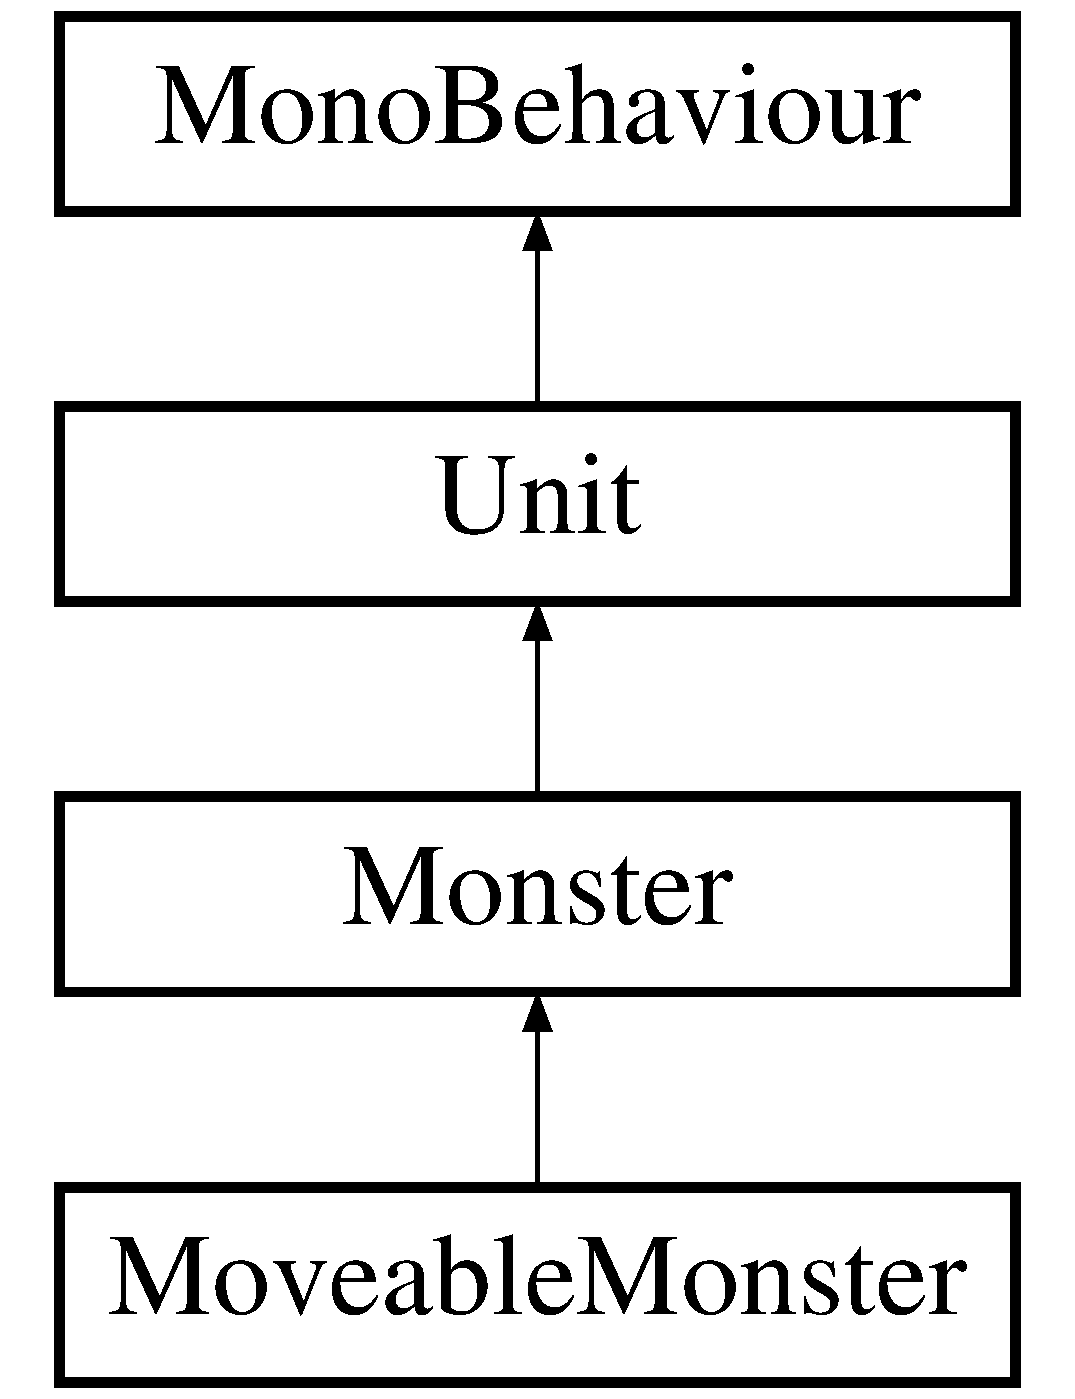
\includegraphics[height=4.000000cm]{class_moveable_monster}
\end{center}
\end{figure}
\subsection*{Protected Member Functions}
\begin{DoxyCompactItemize}
\item 
override void \mbox{\hyperlink{class_moveable_monster_ae4e3c98d944fa303cf1b2c7f4a05a342}{Awake}} ()
\item 
override void \mbox{\hyperlink{class_moveable_monster_a898a6098d4dd0226084e36f3a1c7f093}{Start}} ()
\item 
override void \mbox{\hyperlink{class_moveable_monster_a03035ace68ce00f475ba1ef194ef5595}{Update}} ()
\item 
override void \mbox{\hyperlink{class_moveable_monster_a07aefb0242f24f5b0f2b4cd820b31522}{On\+Trigger\+Enter2D}} (Collider2D collider)
\end{DoxyCompactItemize}
\subsection*{Additional Inherited Members}


\subsection{Member Function Documentation}
\mbox{\Hypertarget{class_moveable_monster_ae4e3c98d944fa303cf1b2c7f4a05a342}\label{class_moveable_monster_ae4e3c98d944fa303cf1b2c7f4a05a342}} 
\index{Moveable\+Monster@{Moveable\+Monster}!Awake@{Awake}}
\index{Awake@{Awake}!Moveable\+Monster@{Moveable\+Monster}}
\subsubsection{\texorpdfstring{Awake()}{Awake()}}
{\footnotesize\ttfamily override void Moveable\+Monster.\+Awake (\begin{DoxyParamCaption}{ }\end{DoxyParamCaption})\hspace{0.3cm}{\ttfamily [inline]}, {\ttfamily [protected]}, {\ttfamily [virtual]}}



Reimplemented from \mbox{\hyperlink{class_monster_a3ccbdc33e8e7e6fb20286338ad17c6f2}{Monster}}.

\mbox{\Hypertarget{class_moveable_monster_a07aefb0242f24f5b0f2b4cd820b31522}\label{class_moveable_monster_a07aefb0242f24f5b0f2b4cd820b31522}} 
\index{Moveable\+Monster@{Moveable\+Monster}!On\+Trigger\+Enter2D@{On\+Trigger\+Enter2D}}
\index{On\+Trigger\+Enter2D@{On\+Trigger\+Enter2D}!Moveable\+Monster@{Moveable\+Monster}}
\subsubsection{\texorpdfstring{On\+Trigger\+Enter2\+D()}{OnTriggerEnter2D()}}
{\footnotesize\ttfamily override void Moveable\+Monster.\+On\+Trigger\+Enter2D (\begin{DoxyParamCaption}\item[{Collider2D}]{collider }\end{DoxyParamCaption})\hspace{0.3cm}{\ttfamily [inline]}, {\ttfamily [protected]}, {\ttfamily [virtual]}}



Reimplemented from \mbox{\hyperlink{class_monster_af6ac6a4c01088e6b4abf79da772cecff}{Monster}}.

\mbox{\Hypertarget{class_moveable_monster_a898a6098d4dd0226084e36f3a1c7f093}\label{class_moveable_monster_a898a6098d4dd0226084e36f3a1c7f093}} 
\index{Moveable\+Monster@{Moveable\+Monster}!Start@{Start}}
\index{Start@{Start}!Moveable\+Monster@{Moveable\+Monster}}
\subsubsection{\texorpdfstring{Start()}{Start()}}
{\footnotesize\ttfamily override void Moveable\+Monster.\+Start (\begin{DoxyParamCaption}{ }\end{DoxyParamCaption})\hspace{0.3cm}{\ttfamily [inline]}, {\ttfamily [protected]}, {\ttfamily [virtual]}}



Reimplemented from \mbox{\hyperlink{class_monster_a79f369a560bdcf5b3dfaf8c9382582d8}{Monster}}.

\mbox{\Hypertarget{class_moveable_monster_a03035ace68ce00f475ba1ef194ef5595}\label{class_moveable_monster_a03035ace68ce00f475ba1ef194ef5595}} 
\index{Moveable\+Monster@{Moveable\+Monster}!Update@{Update}}
\index{Update@{Update}!Moveable\+Monster@{Moveable\+Monster}}
\subsubsection{\texorpdfstring{Update()}{Update()}}
{\footnotesize\ttfamily override void Moveable\+Monster.\+Update (\begin{DoxyParamCaption}{ }\end{DoxyParamCaption})\hspace{0.3cm}{\ttfamily [inline]}, {\ttfamily [protected]}, {\ttfamily [virtual]}}



Reimplemented from \mbox{\hyperlink{class_monster_a91c04bb8ad53b26283de5f5bab20b789}{Monster}}.



The documentation for this class was generated from the following file\+:\begin{DoxyCompactItemize}
\item 
Assets/\+Scripts/\+Monsters/\mbox{\hyperlink{_moveable_monster_8cs}{Moveable\+Monster.\+cs}}\end{DoxyCompactItemize}

\hypertarget{class_moving_object}{}\section{Moving\+Object Class Reference}
\label{class_moving_object}\index{Moving\+Object@{Moving\+Object}}
Inheritance diagram for Moving\+Object\+:\begin{figure}[H]
\begin{center}
\leavevmode
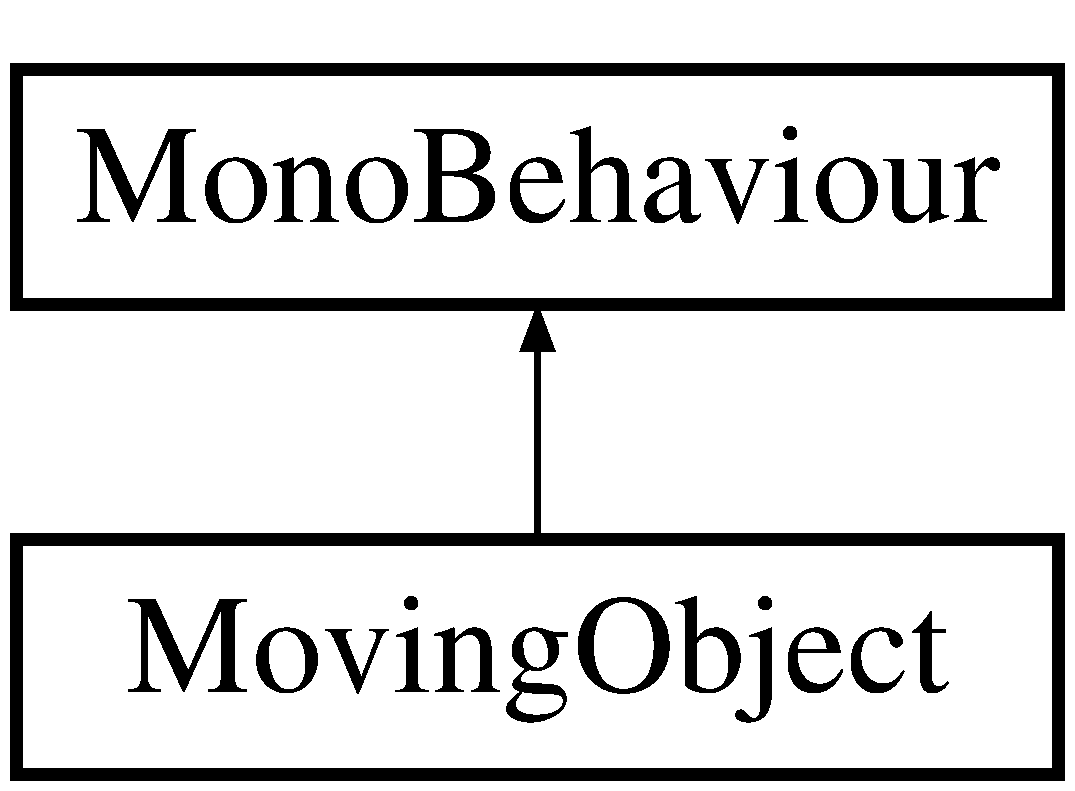
\includegraphics[height=2.000000cm]{class_moving_object}
\end{center}
\end{figure}
\subsection*{Public Attributes}
\begin{DoxyCompactItemize}
\item 
float \mbox{\hyperlink{class_moving_object_a2596eb0312a148176541ac08fb18b173}{move\+Time}} = 0.\+1f
\item 
Layer\+Mask \mbox{\hyperlink{class_moving_object_add4cf20e336559d38cc6a57763775e36}{blocking\+Layer}}
\end{DoxyCompactItemize}
\subsection*{Protected Member Functions}
\begin{DoxyCompactItemize}
\item 
virtual void \mbox{\hyperlink{class_moving_object_a2b6026a8e7e4313764cb876fd99ae1cd}{Start}} ()
\item 
bool \mbox{\hyperlink{class_moving_object_a0a7da7115f17445fcfe898d3ce16b85b}{Move}} (int x\+Dir, int y\+Dir, out Raycast\+Hit2D hit)
\item 
I\+Enumerator \mbox{\hyperlink{class_moving_object_ab5b0553c2da577c976c7f1416ff6605a}{Smooth\+Movement}} (Vector3 end)
\item 
virtual void \mbox{\hyperlink{class_moving_object_a593c3433bf277e5fe6b80ab1b475aad4}{Attempt\+Move$<$ T $>$}} (int x\+Dir, int y\+Dir)
\item 
abstract void \mbox{\hyperlink{class_moving_object_af20de314364d109abfad1fe0f15d4732}{On\+Cant\+Move$<$ T $>$}} (T component)
\end{DoxyCompactItemize}


\subsection{Member Function Documentation}
\mbox{\Hypertarget{class_moving_object_a593c3433bf277e5fe6b80ab1b475aad4}\label{class_moving_object_a593c3433bf277e5fe6b80ab1b475aad4}} 
\index{Moving\+Object@{Moving\+Object}!Attempt\+Move$<$ T $>$@{Attempt\+Move$<$ T $>$}}
\index{Attempt\+Move$<$ T $>$@{Attempt\+Move$<$ T $>$}!Moving\+Object@{Moving\+Object}}
\subsubsection{\texorpdfstring{Attempt\+Move$<$ T $>$()}{AttemptMove< T >()}}
{\footnotesize\ttfamily virtual void Moving\+Object.\+Attempt\+Move$<$ T $>$ (\begin{DoxyParamCaption}\item[{int}]{x\+Dir,  }\item[{int}]{y\+Dir }\end{DoxyParamCaption})\hspace{0.3cm}{\ttfamily [inline]}, {\ttfamily [protected]}, {\ttfamily [virtual]}}

\begin{Desc}
\item[Type Constraints]\begin{description}
\item[{\em T} : {\em Component}]\end{description}
\end{Desc}
\mbox{\Hypertarget{class_moving_object_a0a7da7115f17445fcfe898d3ce16b85b}\label{class_moving_object_a0a7da7115f17445fcfe898d3ce16b85b}} 
\index{Moving\+Object@{Moving\+Object}!Move@{Move}}
\index{Move@{Move}!Moving\+Object@{Moving\+Object}}
\subsubsection{\texorpdfstring{Move()}{Move()}}
{\footnotesize\ttfamily bool Moving\+Object.\+Move (\begin{DoxyParamCaption}\item[{int}]{x\+Dir,  }\item[{int}]{y\+Dir,  }\item[{out Raycast\+Hit2D}]{hit }\end{DoxyParamCaption})\hspace{0.3cm}{\ttfamily [inline]}, {\ttfamily [protected]}}

\mbox{\Hypertarget{class_moving_object_af20de314364d109abfad1fe0f15d4732}\label{class_moving_object_af20de314364d109abfad1fe0f15d4732}} 
\index{Moving\+Object@{Moving\+Object}!On\+Cant\+Move$<$ T $>$@{On\+Cant\+Move$<$ T $>$}}
\index{On\+Cant\+Move$<$ T $>$@{On\+Cant\+Move$<$ T $>$}!Moving\+Object@{Moving\+Object}}
\subsubsection{\texorpdfstring{On\+Cant\+Move$<$ T $>$()}{OnCantMove< T >()}}
{\footnotesize\ttfamily abstract void Moving\+Object.\+On\+Cant\+Move$<$ T $>$ (\begin{DoxyParamCaption}\item[{T}]{component }\end{DoxyParamCaption})\hspace{0.3cm}{\ttfamily [protected]}, {\ttfamily [pure virtual]}}

\begin{Desc}
\item[Type Constraints]\begin{description}
\item[{\em T} : {\em Component}]\end{description}
\end{Desc}
\mbox{\Hypertarget{class_moving_object_ab5b0553c2da577c976c7f1416ff6605a}\label{class_moving_object_ab5b0553c2da577c976c7f1416ff6605a}} 
\index{Moving\+Object@{Moving\+Object}!Smooth\+Movement@{Smooth\+Movement}}
\index{Smooth\+Movement@{Smooth\+Movement}!Moving\+Object@{Moving\+Object}}
\subsubsection{\texorpdfstring{Smooth\+Movement()}{SmoothMovement()}}
{\footnotesize\ttfamily I\+Enumerator Moving\+Object.\+Smooth\+Movement (\begin{DoxyParamCaption}\item[{Vector3}]{end }\end{DoxyParamCaption})\hspace{0.3cm}{\ttfamily [inline]}, {\ttfamily [protected]}}

\mbox{\Hypertarget{class_moving_object_a2b6026a8e7e4313764cb876fd99ae1cd}\label{class_moving_object_a2b6026a8e7e4313764cb876fd99ae1cd}} 
\index{Moving\+Object@{Moving\+Object}!Start@{Start}}
\index{Start@{Start}!Moving\+Object@{Moving\+Object}}
\subsubsection{\texorpdfstring{Start()}{Start()}}
{\footnotesize\ttfamily virtual void Moving\+Object.\+Start (\begin{DoxyParamCaption}{ }\end{DoxyParamCaption})\hspace{0.3cm}{\ttfamily [inline]}, {\ttfamily [protected]}, {\ttfamily [virtual]}}



\subsection{Member Data Documentation}
\mbox{\Hypertarget{class_moving_object_add4cf20e336559d38cc6a57763775e36}\label{class_moving_object_add4cf20e336559d38cc6a57763775e36}} 
\index{Moving\+Object@{Moving\+Object}!blocking\+Layer@{blocking\+Layer}}
\index{blocking\+Layer@{blocking\+Layer}!Moving\+Object@{Moving\+Object}}
\subsubsection{\texorpdfstring{blocking\+Layer}{blockingLayer}}
{\footnotesize\ttfamily Layer\+Mask Moving\+Object.\+blocking\+Layer}

\mbox{\Hypertarget{class_moving_object_a2596eb0312a148176541ac08fb18b173}\label{class_moving_object_a2596eb0312a148176541ac08fb18b173}} 
\index{Moving\+Object@{Moving\+Object}!move\+Time@{move\+Time}}
\index{move\+Time@{move\+Time}!Moving\+Object@{Moving\+Object}}
\subsubsection{\texorpdfstring{move\+Time}{moveTime}}
{\footnotesize\ttfamily float Moving\+Object.\+move\+Time = 0.\+1f}



The documentation for this class was generated from the following file\+:\begin{DoxyCompactItemize}
\item 
Assets/\+Scripts/\+Objects/\mbox{\hyperlink{_moving_object_8cs}{Moving\+Object.\+cs}}\end{DoxyCompactItemize}

\hypertarget{class_new_game_button}{}\section{New\+Game\+Button Class Reference}
\label{class_new_game_button}\index{New\+Game\+Button@{New\+Game\+Button}}


Класс, функция которого -\/ переход на следующую сцену  


Inheritance diagram for New\+Game\+Button\+:\begin{figure}[H]
\begin{center}
\leavevmode
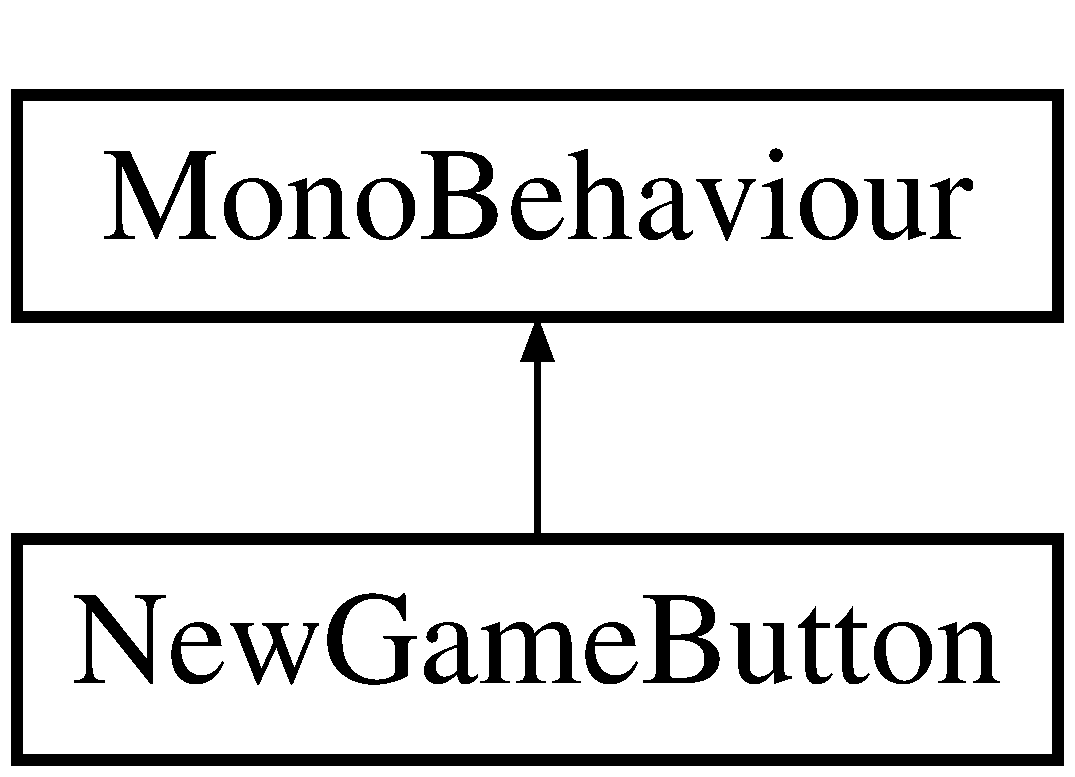
\includegraphics[height=2.000000cm]{class_new_game_button}
\end{center}
\end{figure}
\subsection*{Public Member Functions}
\begin{DoxyCompactItemize}
\item 
void \mbox{\hyperlink{class_new_game_button_aec7029f42fc0de5cf7f50952f3b4d3fd}{Load\+High\+Score\+Level}} ()
\begin{DoxyCompactList}\small\item\em Функция загрузки сцены по переменной name\+Level \end{DoxyCompactList}\end{DoxyCompactItemize}


\subsection{Detailed Description}
Класс, функция которого -\/ переход на следующую сцену 



\subsection{Member Function Documentation}
\mbox{\Hypertarget{class_new_game_button_aec7029f42fc0de5cf7f50952f3b4d3fd}\label{class_new_game_button_aec7029f42fc0de5cf7f50952f3b4d3fd}} 
\index{New\+Game\+Button@{New\+Game\+Button}!Load\+High\+Score\+Level@{Load\+High\+Score\+Level}}
\index{Load\+High\+Score\+Level@{Load\+High\+Score\+Level}!New\+Game\+Button@{New\+Game\+Button}}
\subsubsection{\texorpdfstring{Load\+High\+Score\+Level()}{LoadHighScoreLevel()}}
{\footnotesize\ttfamily void New\+Game\+Button.\+Load\+High\+Score\+Level (\begin{DoxyParamCaption}{ }\end{DoxyParamCaption})\hspace{0.3cm}{\ttfamily [inline]}}



Функция загрузки сцены по переменной name\+Level 



The documentation for this class was generated from the following file\+:\begin{DoxyCompactItemize}
\item 
Assets/\+Scripts/\+Buttons/\mbox{\hyperlink{_new_game_button_8cs}{New\+Game\+Button.\+cs}}\end{DoxyCompactItemize}

\hypertarget{class_obstacle}{}\section{Obstacle Class Reference}
\label{class_obstacle}\index{Obstacle@{Obstacle}}
Inheritance diagram for Obstacle\+:\begin{figure}[H]
\begin{center}
\leavevmode
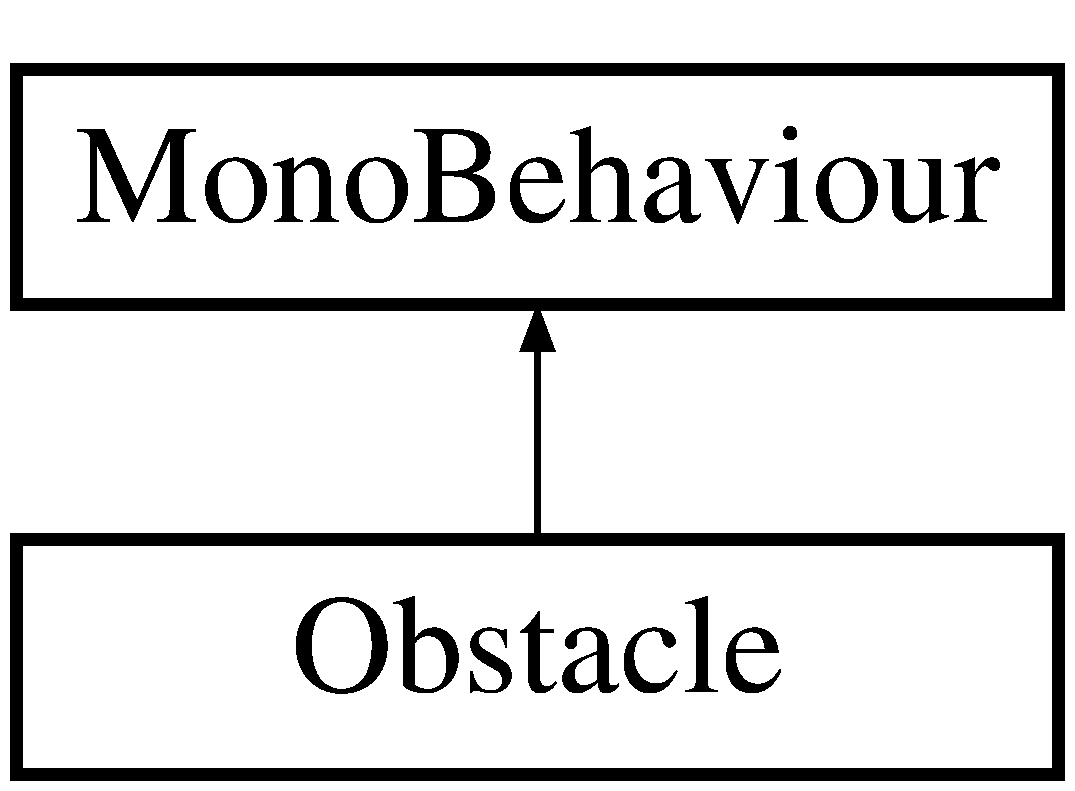
\includegraphics[height=2.000000cm]{class_obstacle}
\end{center}
\end{figure}


The documentation for this class was generated from the following file\+:\begin{DoxyCompactItemize}
\item 
Assets/\+Scripts/\+Monsters/\mbox{\hyperlink{_obstacle_8cs}{Obstacle.\+cs}}\end{DoxyCompactItemize}

\hypertarget{class_ornament}{}\section{Ornament Class Reference}
\label{class_ornament}\index{Ornament@{Ornament}}
Inheritance diagram for Ornament\+:\begin{figure}[H]
\begin{center}
\leavevmode
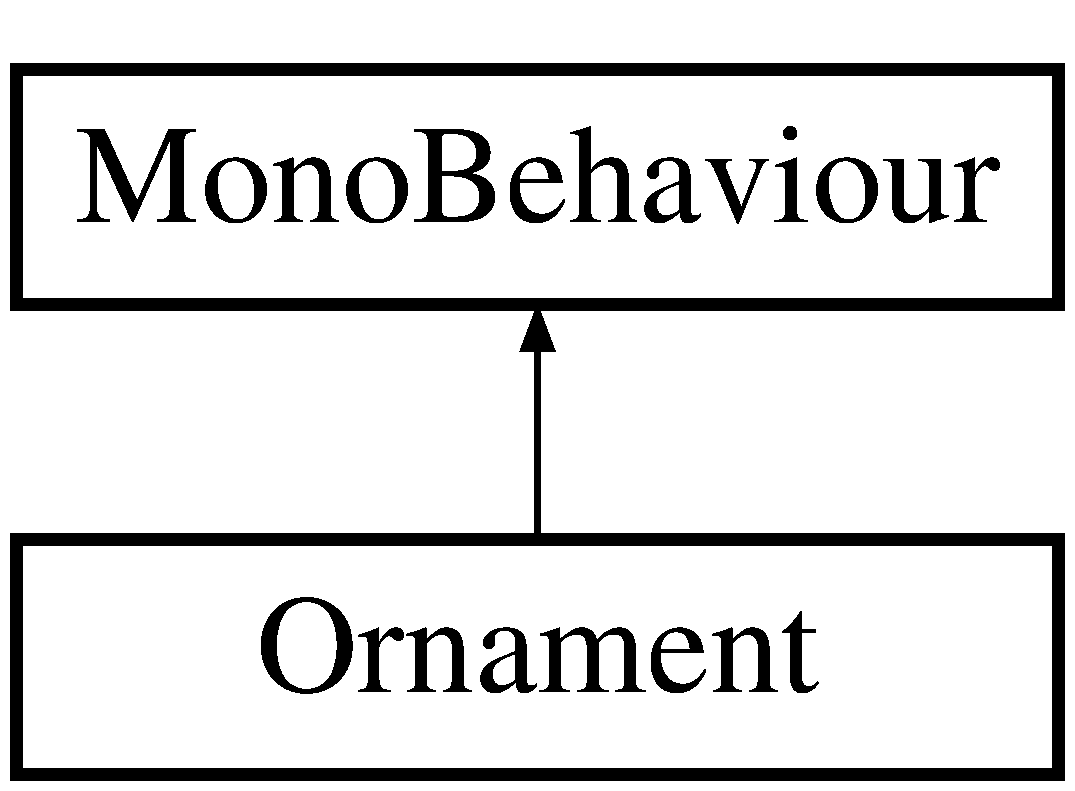
\includegraphics[height=2.000000cm]{class_ornament}
\end{center}
\end{figure}
\subsection*{Public Attributes}
\begin{DoxyCompactItemize}
\item 
bool \mbox{\hyperlink{class_ornament_abbdf4ce334356bac00965b2e72f4c0b1}{locked}}
\end{DoxyCompactItemize}


\subsection{Member Data Documentation}
\mbox{\Hypertarget{class_ornament_abbdf4ce334356bac00965b2e72f4c0b1}\label{class_ornament_abbdf4ce334356bac00965b2e72f4c0b1}} 
\index{Ornament@{Ornament}!locked@{locked}}
\index{locked@{locked}!Ornament@{Ornament}}
\subsubsection{\texorpdfstring{locked}{locked}}
{\footnotesize\ttfamily bool Ornament.\+locked}



The documentation for this class was generated from the following file\+:\begin{DoxyCompactItemize}
\item 
Assets/\+Scripts/\+Puzzle\+Game/\mbox{\hyperlink{_ornament_8cs}{Ornament.\+cs}}\end{DoxyCompactItemize}

\hypertarget{class_ornament_manager}{}\section{Ornament\+Manager Class Reference}
\label{class_ornament_manager}\index{Ornament\+Manager@{Ornament\+Manager}}
Inheritance diagram for Ornament\+Manager\+:\begin{figure}[H]
\begin{center}
\leavevmode
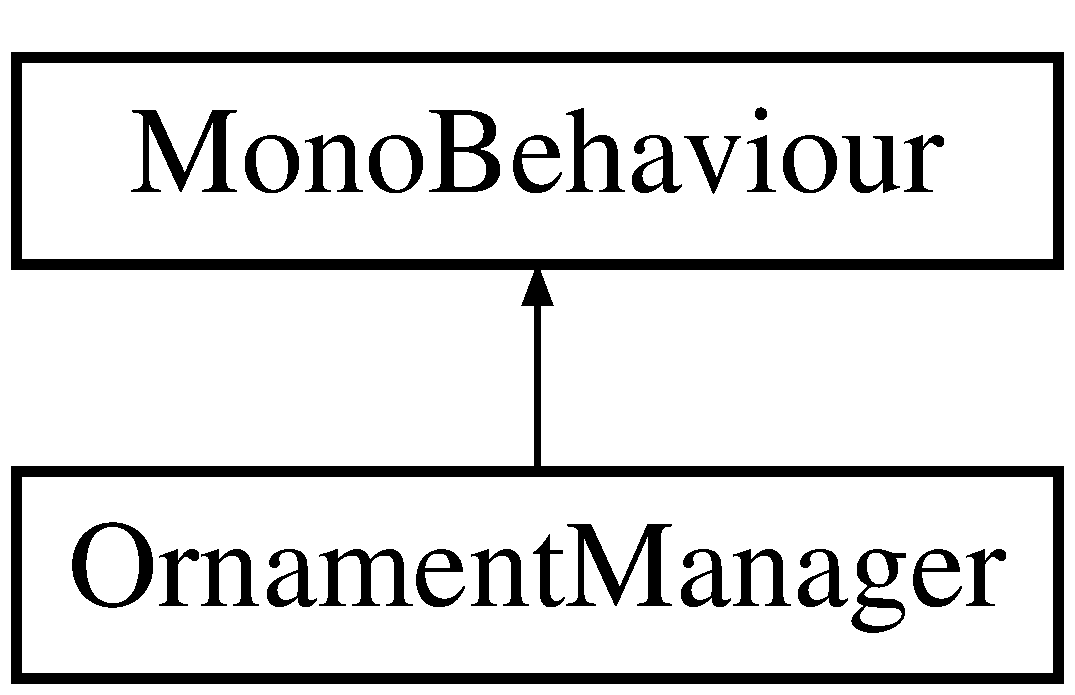
\includegraphics[height=2.000000cm]{class_ornament_manager}
\end{center}
\end{figure}
\subsection*{Public Attributes}
\begin{DoxyCompactItemize}
\item 
Game\+Object \mbox{\hyperlink{class_ornament_manager_a774b255d77938f0e0172b62a334f3c90}{panel}}
\item 
\mbox{\hyperlink{class_ornament}{Ornament}} \mbox{[}$\,$\mbox{]} \mbox{\hyperlink{class_ornament_manager_ab4161a70592b59370a110f6e0b47b84f}{\+\_\+puzzle}}
\item 
bool \mbox{\hyperlink{class_ornament_manager_a5e8539e721f6c95e3f6d080851dc1219}{well\+Done}} = false
\end{DoxyCompactItemize}


\subsection{Member Data Documentation}
\mbox{\Hypertarget{class_ornament_manager_ab4161a70592b59370a110f6e0b47b84f}\label{class_ornament_manager_ab4161a70592b59370a110f6e0b47b84f}} 
\index{Ornament\+Manager@{Ornament\+Manager}!\+\_\+puzzle@{\+\_\+puzzle}}
\index{\+\_\+puzzle@{\+\_\+puzzle}!Ornament\+Manager@{Ornament\+Manager}}
\subsubsection{\texorpdfstring{\+\_\+puzzle}{\_puzzle}}
{\footnotesize\ttfamily \mbox{\hyperlink{class_ornament}{Ornament}} \mbox{[}$\,$\mbox{]} Ornament\+Manager.\+\_\+puzzle}

\mbox{\Hypertarget{class_ornament_manager_a774b255d77938f0e0172b62a334f3c90}\label{class_ornament_manager_a774b255d77938f0e0172b62a334f3c90}} 
\index{Ornament\+Manager@{Ornament\+Manager}!panel@{panel}}
\index{panel@{panel}!Ornament\+Manager@{Ornament\+Manager}}
\subsubsection{\texorpdfstring{panel}{panel}}
{\footnotesize\ttfamily Game\+Object Ornament\+Manager.\+panel}

\mbox{\Hypertarget{class_ornament_manager_a5e8539e721f6c95e3f6d080851dc1219}\label{class_ornament_manager_a5e8539e721f6c95e3f6d080851dc1219}} 
\index{Ornament\+Manager@{Ornament\+Manager}!well\+Done@{well\+Done}}
\index{well\+Done@{well\+Done}!Ornament\+Manager@{Ornament\+Manager}}
\subsubsection{\texorpdfstring{well\+Done}{wellDone}}
{\footnotesize\ttfamily bool Ornament\+Manager.\+well\+Done = false}



The documentation for this class was generated from the following file\+:\begin{DoxyCompactItemize}
\item 
Assets/\+Scripts/\+Puzzle\+Game/\mbox{\hyperlink{_ornament_manager_8cs}{Ornament\+Manager.\+cs}}\end{DoxyCompactItemize}

\hypertarget{class_pause}{}\section{Pause Class Reference}
\label{class_pause}\index{Pause@{Pause}}
Inheritance diagram for Pause\+:\begin{figure}[H]
\begin{center}
\leavevmode
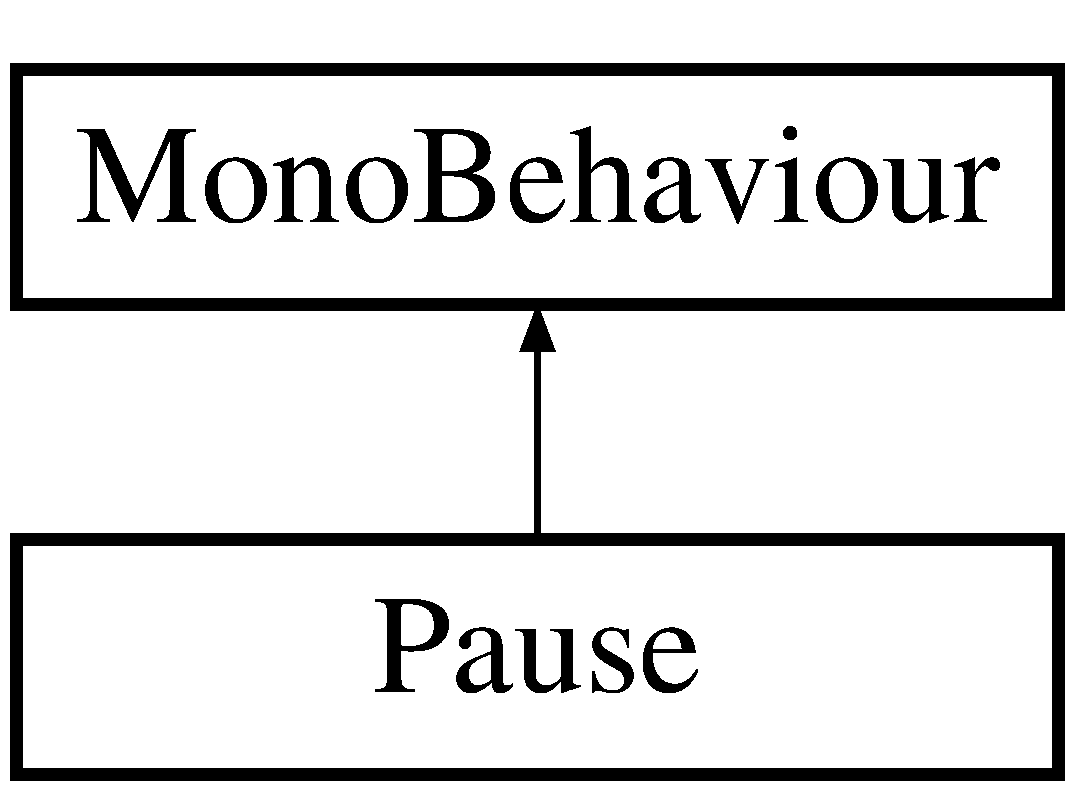
\includegraphics[height=2.000000cm]{class_pause}
\end{center}
\end{figure}
\subsection*{Public Attributes}
\begin{DoxyCompactItemize}
\item 
bool \mbox{\hyperlink{class_pause_ae845c846c4be05e29c8948089f57eec0}{is\+Paused}} = false
\end{DoxyCompactItemize}


\subsection{Member Data Documentation}
\mbox{\Hypertarget{class_pause_ae845c846c4be05e29c8948089f57eec0}\label{class_pause_ae845c846c4be05e29c8948089f57eec0}} 
\index{Pause@{Pause}!is\+Paused@{is\+Paused}}
\index{is\+Paused@{is\+Paused}!Pause@{Pause}}
\subsubsection{\texorpdfstring{is\+Paused}{isPaused}}
{\footnotesize\ttfamily bool Pause.\+is\+Paused = false}



The documentation for this class was generated from the following file\+:\begin{DoxyCompactItemize}
\item 
Assets/\+Scripts/\+Buttons/\mbox{\hyperlink{_pause_8cs}{Pause.\+cs}}\end{DoxyCompactItemize}

\hypertarget{class_portal}{}\section{Portal Class Reference}
\label{class_portal}\index{Portal@{Portal}}
Inheritance diagram for Portal\+:\begin{figure}[H]
\begin{center}
\leavevmode
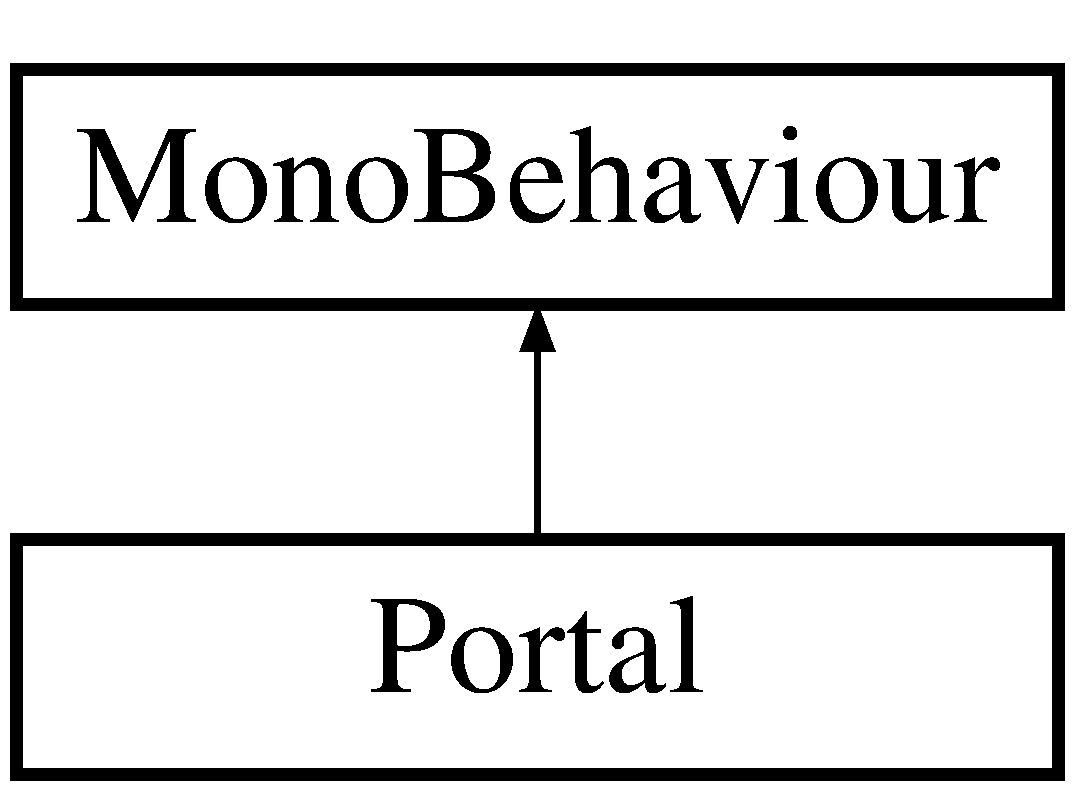
\includegraphics[height=2.000000cm]{class_portal}
\end{center}
\end{figure}


The documentation for this class was generated from the following file\+:\begin{DoxyCompactItemize}
\item 
Assets/\+Scripts/\+Objects/\mbox{\hyperlink{_portal_8cs}{Portal.\+cs}}\end{DoxyCompactItemize}

\hypertarget{class_puzzle}{}\section{Puzzle Class Reference}
\label{class_puzzle}\index{Puzzle@{Puzzle}}
Inheritance diagram for Puzzle\+:\begin{figure}[H]
\begin{center}
\leavevmode
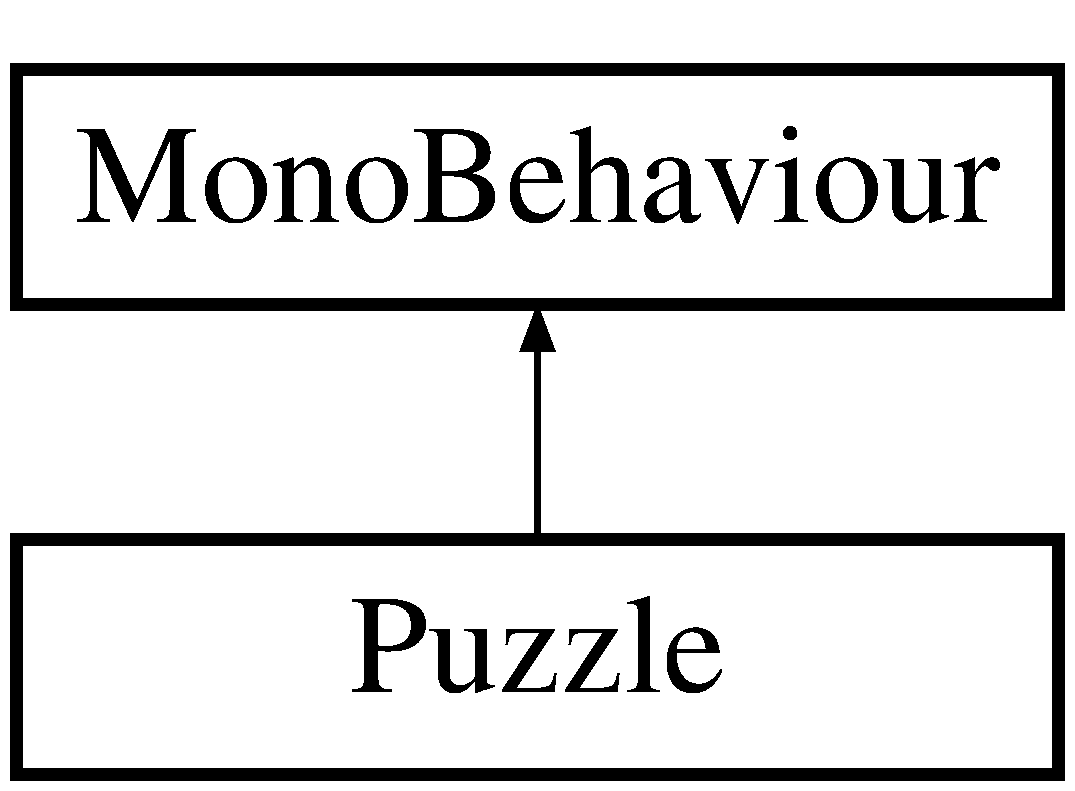
\includegraphics[height=2.000000cm]{class_puzzle}
\end{center}
\end{figure}
\subsection*{Public Attributes}
\begin{DoxyCompactItemize}
\item 
int \mbox{\hyperlink{class_puzzle_a3570b0062c358cd4b94c923cffd40130}{ID}}
\end{DoxyCompactItemize}


\subsection{Member Data Documentation}
\mbox{\Hypertarget{class_puzzle_a3570b0062c358cd4b94c923cffd40130}\label{class_puzzle_a3570b0062c358cd4b94c923cffd40130}} 
\index{Puzzle@{Puzzle}!ID@{ID}}
\index{ID@{ID}!Puzzle@{Puzzle}}
\subsubsection{\texorpdfstring{ID}{ID}}
{\footnotesize\ttfamily int Puzzle.\+ID}



The documentation for this class was generated from the following file\+:\begin{DoxyCompactItemize}
\item 
Assets/\+Scripts/\+Chess\+Game/\mbox{\hyperlink{_puzzle_8cs}{Puzzle.\+cs}}\end{DoxyCompactItemize}

\hypertarget{class_quit}{}\section{Quit Class Reference}
\label{class_quit}\index{Quit@{Quit}}
Inheritance diagram for Quit\+:\begin{figure}[H]
\begin{center}
\leavevmode
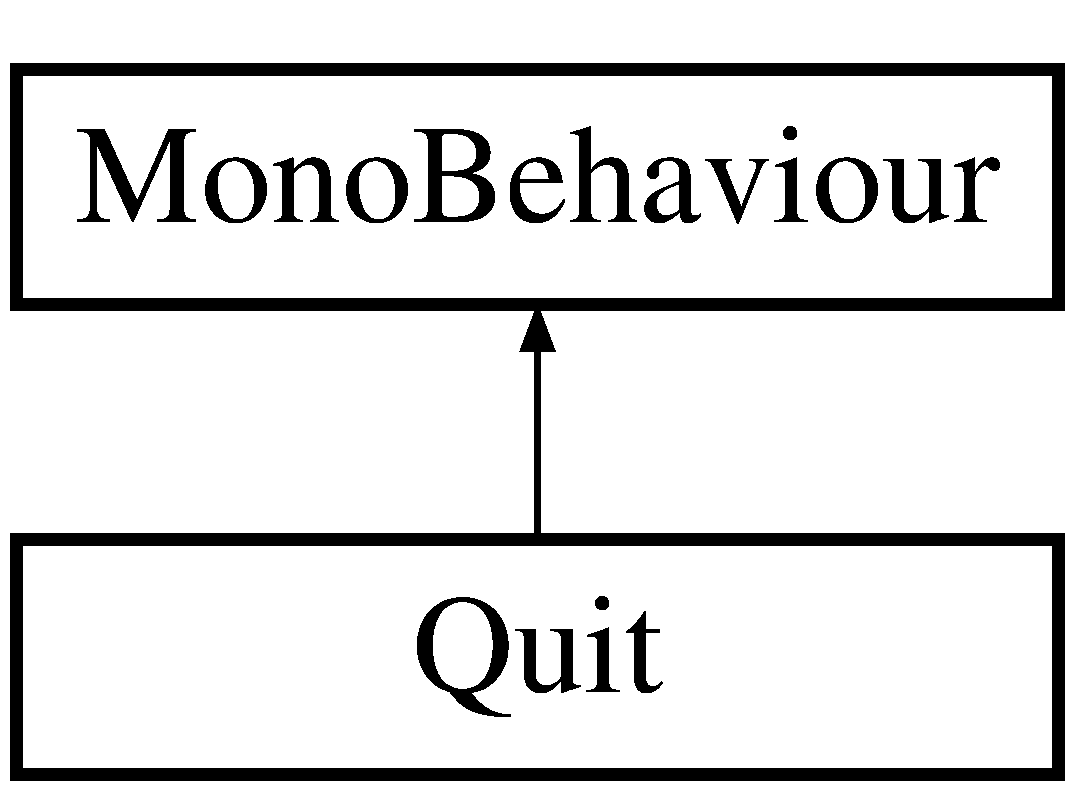
\includegraphics[height=2.000000cm]{class_quit}
\end{center}
\end{figure}
\subsection*{Public Member Functions}
\begin{DoxyCompactItemize}
\item 
void \mbox{\hyperlink{class_quit_ab9e748ddc8aeb84ce108116c22ac5804}{Exit}} ()
\end{DoxyCompactItemize}


\subsection{Member Function Documentation}
\mbox{\Hypertarget{class_quit_ab9e748ddc8aeb84ce108116c22ac5804}\label{class_quit_ab9e748ddc8aeb84ce108116c22ac5804}} 
\index{Quit@{Quit}!Exit@{Exit}}
\index{Exit@{Exit}!Quit@{Quit}}
\subsubsection{\texorpdfstring{Exit()}{Exit()}}
{\footnotesize\ttfamily void Quit.\+Exit (\begin{DoxyParamCaption}{ }\end{DoxyParamCaption})\hspace{0.3cm}{\ttfamily [inline]}}



The documentation for this class was generated from the following file\+:\begin{DoxyCompactItemize}
\item 
Assets/\+Scripts/\+Buttons/\mbox{\hyperlink{_quit_8cs}{Quit.\+cs}}\end{DoxyCompactItemize}

\hypertarget{class_reload}{}\section{Reload Class Reference}
\label{class_reload}\index{Reload@{Reload}}
Inheritance diagram for Reload\+:\begin{figure}[H]
\begin{center}
\leavevmode
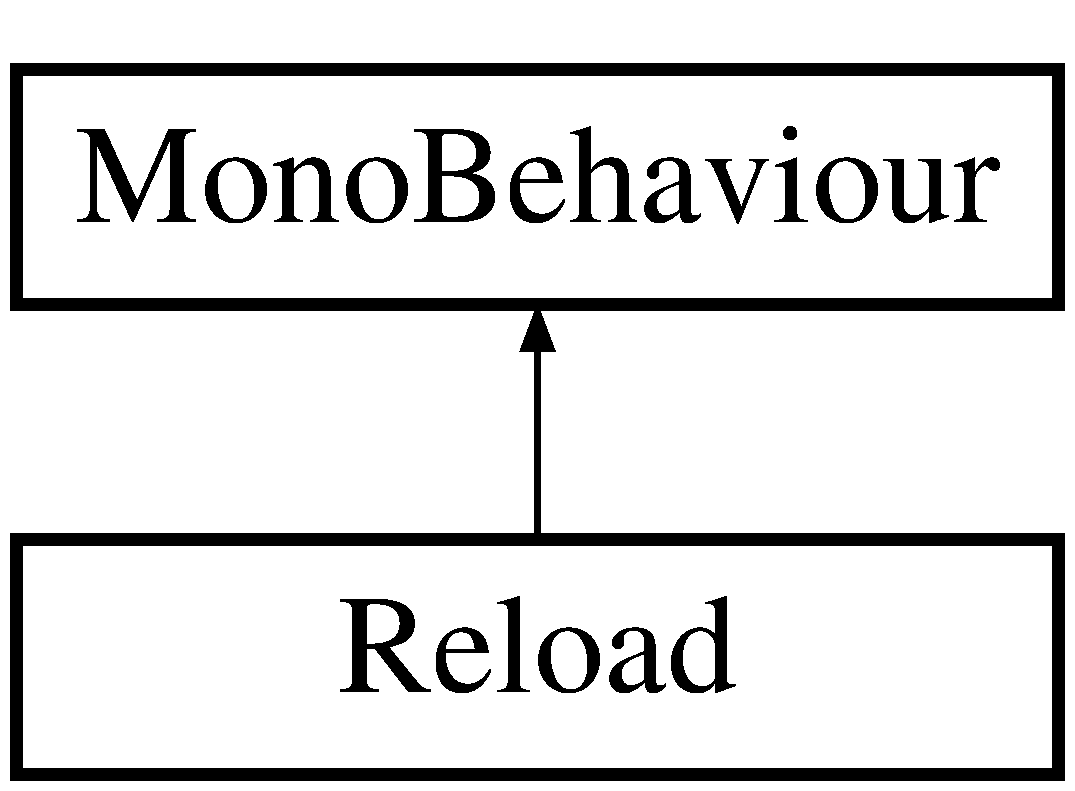
\includegraphics[height=2.000000cm]{class_reload}
\end{center}
\end{figure}
\subsection*{Public Member Functions}
\begin{DoxyCompactItemize}
\item 
void \mbox{\hyperlink{class_reload_a196037885896ca2a3d05e11eb75fcdb1}{Re}} ()
\end{DoxyCompactItemize}
\subsection*{Public Attributes}
\begin{DoxyCompactItemize}
\item 
string \mbox{\hyperlink{class_reload_a1c7abc2a97caa3db3217948dcd0f3da5}{name}} = \char`\"{}Chess\+Game\char`\"{}
\end{DoxyCompactItemize}


\subsection{Member Function Documentation}
\mbox{\Hypertarget{class_reload_a196037885896ca2a3d05e11eb75fcdb1}\label{class_reload_a196037885896ca2a3d05e11eb75fcdb1}} 
\index{Reload@{Reload}!Re@{Re}}
\index{Re@{Re}!Reload@{Reload}}
\subsubsection{\texorpdfstring{Re()}{Re()}}
{\footnotesize\ttfamily void Reload.\+Re (\begin{DoxyParamCaption}{ }\end{DoxyParamCaption})\hspace{0.3cm}{\ttfamily [inline]}}



\subsection{Member Data Documentation}
\mbox{\Hypertarget{class_reload_a1c7abc2a97caa3db3217948dcd0f3da5}\label{class_reload_a1c7abc2a97caa3db3217948dcd0f3da5}} 
\index{Reload@{Reload}!name@{name}}
\index{name@{name}!Reload@{Reload}}
\subsubsection{\texorpdfstring{name}{name}}
{\footnotesize\ttfamily string Reload.\+name = \char`\"{}Chess\+Game\char`\"{}}



The documentation for this class was generated from the following file\+:\begin{DoxyCompactItemize}
\item 
Assets/\+Scripts/\+Buttons/\mbox{\hyperlink{_reload_8cs}{Reload.\+cs}}\end{DoxyCompactItemize}

\hypertarget{class_shield}{}\section{Shield Class Reference}
\label{class_shield}\index{Shield@{Shield}}
Inheritance diagram for Shield\+:\begin{figure}[H]
\begin{center}
\leavevmode
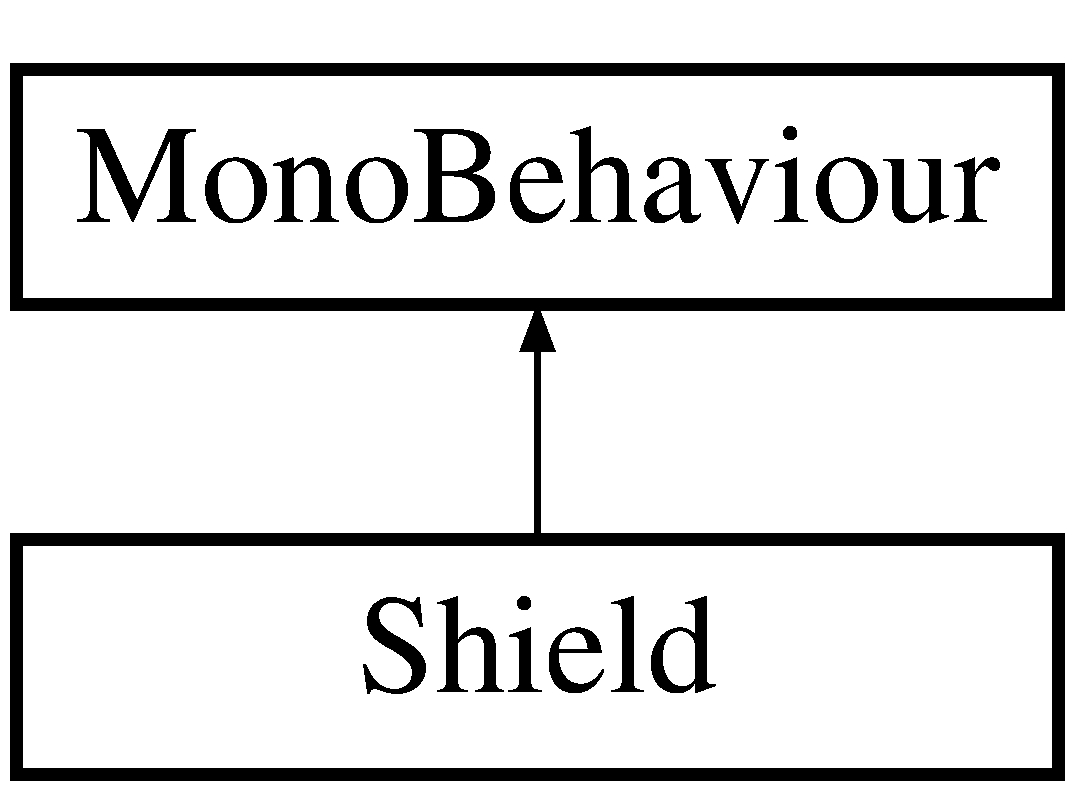
\includegraphics[height=2.000000cm]{class_shield}
\end{center}
\end{figure}


The documentation for this class was generated from the following file\+:\begin{DoxyCompactItemize}
\item 
Assets/\+Scripts/\mbox{\hyperlink{_shield_8cs}{Shield.\+cs}}\end{DoxyCompactItemize}

\hypertarget{class_shootable_monster}{}\section{Shootable\+Monster Class Reference}
\label{class_shootable_monster}\index{Shootable\+Monster@{Shootable\+Monster}}
Inheritance diagram for Shootable\+Monster\+:\begin{figure}[H]
\begin{center}
\leavevmode
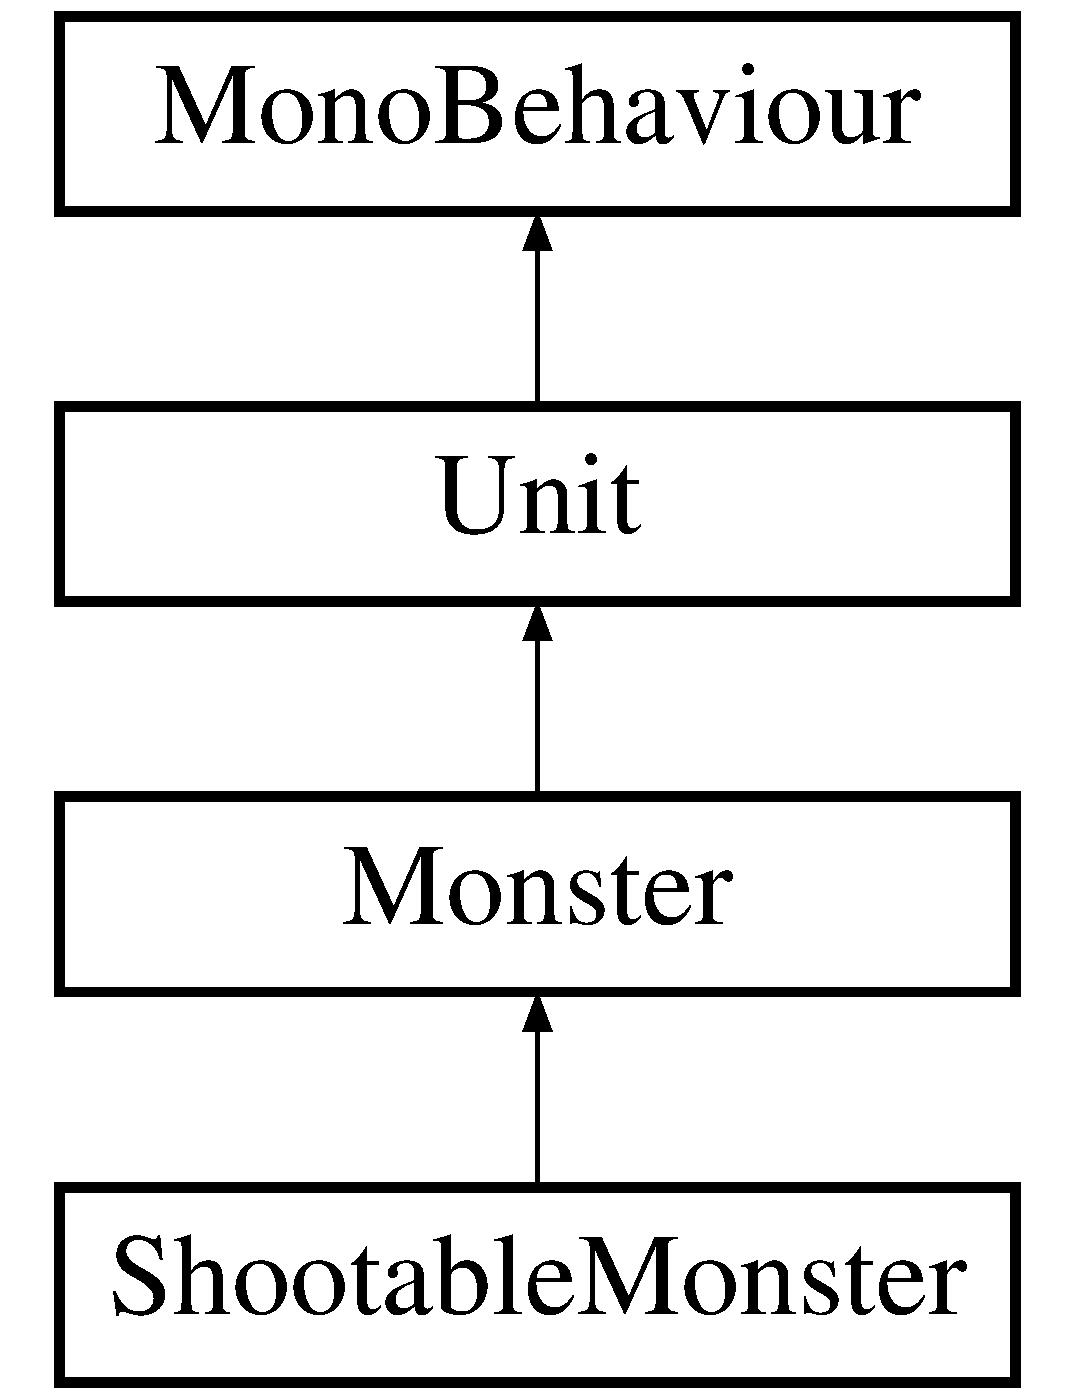
\includegraphics[height=4.000000cm]{class_shootable_monster}
\end{center}
\end{figure}
\subsection*{Public Attributes}
\begin{DoxyCompactItemize}
\item 
float \mbox{\hyperlink{class_shootable_monster_a3dc33446a2d7405d4c0f49de76c4961d}{positionY}} = 0.\+5F
\end{DoxyCompactItemize}
\subsection*{Protected Member Functions}
\begin{DoxyCompactItemize}
\item 
override void \mbox{\hyperlink{class_shootable_monster_adfb9638b7a397563df4ab94c2db20ec0}{Awake}} ()
\item 
override void \mbox{\hyperlink{class_shootable_monster_a0e26de95298ec75a591ecede3c1d8cb9}{Start}} ()
\item 
override void \mbox{\hyperlink{class_shootable_monster_a6c350a976d1bb37db2c663834c90e83b}{On\+Trigger\+Enter2D}} (Collider2D collider)
\end{DoxyCompactItemize}
\subsection*{Additional Inherited Members}


\subsection{Member Function Documentation}
\mbox{\Hypertarget{class_shootable_monster_adfb9638b7a397563df4ab94c2db20ec0}\label{class_shootable_monster_adfb9638b7a397563df4ab94c2db20ec0}} 
\index{Shootable\+Monster@{Shootable\+Monster}!Awake@{Awake}}
\index{Awake@{Awake}!Shootable\+Monster@{Shootable\+Monster}}
\subsubsection{\texorpdfstring{Awake()}{Awake()}}
{\footnotesize\ttfamily override void Shootable\+Monster.\+Awake (\begin{DoxyParamCaption}{ }\end{DoxyParamCaption})\hspace{0.3cm}{\ttfamily [inline]}, {\ttfamily [protected]}, {\ttfamily [virtual]}}



Reimplemented from \mbox{\hyperlink{class_monster_a3ccbdc33e8e7e6fb20286338ad17c6f2}{Monster}}.

\mbox{\Hypertarget{class_shootable_monster_a6c350a976d1bb37db2c663834c90e83b}\label{class_shootable_monster_a6c350a976d1bb37db2c663834c90e83b}} 
\index{Shootable\+Monster@{Shootable\+Monster}!On\+Trigger\+Enter2D@{On\+Trigger\+Enter2D}}
\index{On\+Trigger\+Enter2D@{On\+Trigger\+Enter2D}!Shootable\+Monster@{Shootable\+Monster}}
\subsubsection{\texorpdfstring{On\+Trigger\+Enter2\+D()}{OnTriggerEnter2D()}}
{\footnotesize\ttfamily override void Shootable\+Monster.\+On\+Trigger\+Enter2D (\begin{DoxyParamCaption}\item[{Collider2D}]{collider }\end{DoxyParamCaption})\hspace{0.3cm}{\ttfamily [inline]}, {\ttfamily [protected]}, {\ttfamily [virtual]}}



Reimplemented from \mbox{\hyperlink{class_monster_af6ac6a4c01088e6b4abf79da772cecff}{Monster}}.

\mbox{\Hypertarget{class_shootable_monster_a0e26de95298ec75a591ecede3c1d8cb9}\label{class_shootable_monster_a0e26de95298ec75a591ecede3c1d8cb9}} 
\index{Shootable\+Monster@{Shootable\+Monster}!Start@{Start}}
\index{Start@{Start}!Shootable\+Monster@{Shootable\+Monster}}
\subsubsection{\texorpdfstring{Start()}{Start()}}
{\footnotesize\ttfamily override void Shootable\+Monster.\+Start (\begin{DoxyParamCaption}{ }\end{DoxyParamCaption})\hspace{0.3cm}{\ttfamily [inline]}, {\ttfamily [protected]}, {\ttfamily [virtual]}}



Reimplemented from \mbox{\hyperlink{class_monster_a79f369a560bdcf5b3dfaf8c9382582d8}{Monster}}.



\subsection{Member Data Documentation}
\mbox{\Hypertarget{class_shootable_monster_a3dc33446a2d7405d4c0f49de76c4961d}\label{class_shootable_monster_a3dc33446a2d7405d4c0f49de76c4961d}} 
\index{Shootable\+Monster@{Shootable\+Monster}!positionY@{positionY}}
\index{positionY@{positionY}!Shootable\+Monster@{Shootable\+Monster}}
\subsubsection{\texorpdfstring{positionY}{positionY}}
{\footnotesize\ttfamily float Shootable\+Monster.\+positionY = 0.\+5F}



The documentation for this class was generated from the following file\+:\begin{DoxyCompactItemize}
\item 
Assets/\+Scripts/\+Monsters/\mbox{\hyperlink{_shootable_monster_8cs}{Shootable\+Monster.\+cs}}\end{DoxyCompactItemize}

\hypertarget{class_show_button}{}\section{Show\+Button Class Reference}
\label{class_show_button}\index{Show\+Button@{Show\+Button}}
Inheritance diagram for Show\+Button\+:\begin{figure}[H]
\begin{center}
\leavevmode
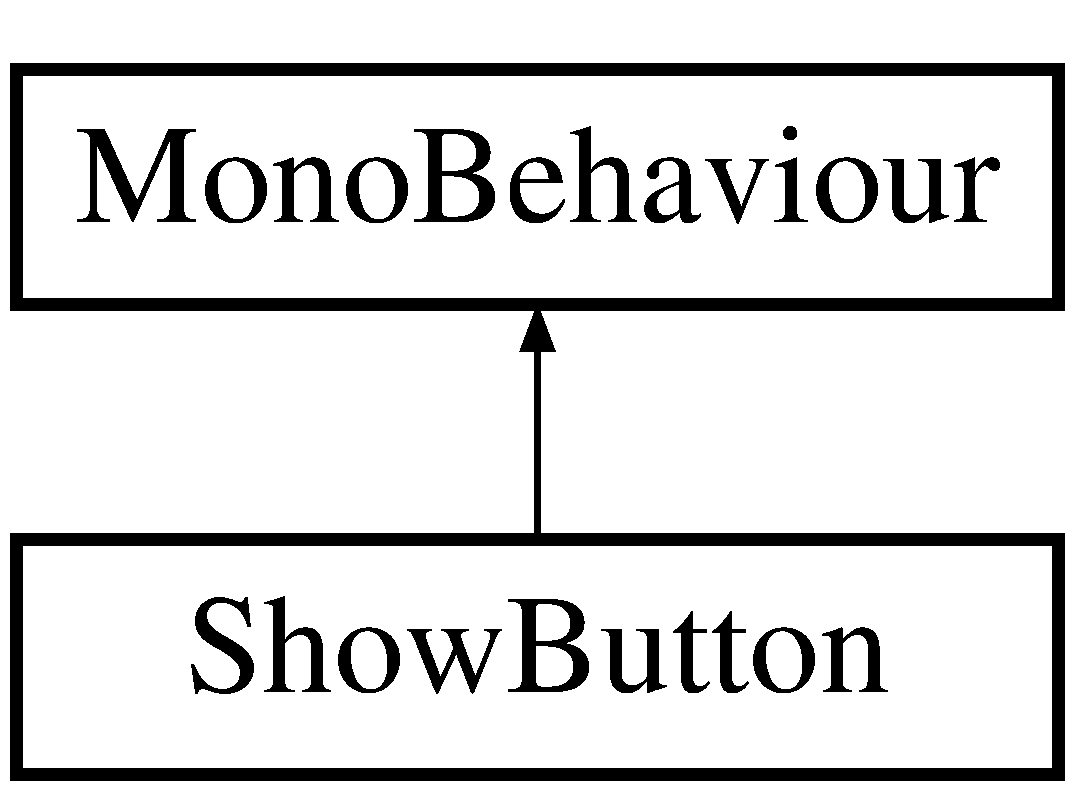
\includegraphics[height=2.000000cm]{class_show_button}
\end{center}
\end{figure}
\subsection*{Public Member Functions}
\begin{DoxyCompactItemize}
\item 
void \mbox{\hyperlink{class_show_button_a8f2bd61ba16b46b401390a7357cf8249}{Show}} ()
\end{DoxyCompactItemize}
\subsection*{Public Attributes}
\begin{DoxyCompactItemize}
\item 
bool \mbox{\hyperlink{class_show_button_abda8b88daac10df3fe20c640360fcaab}{is\+Paused}} = false
\end{DoxyCompactItemize}


\subsection{Member Function Documentation}
\mbox{\Hypertarget{class_show_button_a8f2bd61ba16b46b401390a7357cf8249}\label{class_show_button_a8f2bd61ba16b46b401390a7357cf8249}} 
\index{Show\+Button@{Show\+Button}!Show@{Show}}
\index{Show@{Show}!Show\+Button@{Show\+Button}}
\subsubsection{\texorpdfstring{Show()}{Show()}}
{\footnotesize\ttfamily void Show\+Button.\+Show (\begin{DoxyParamCaption}{ }\end{DoxyParamCaption})\hspace{0.3cm}{\ttfamily [inline]}}



\subsection{Member Data Documentation}
\mbox{\Hypertarget{class_show_button_abda8b88daac10df3fe20c640360fcaab}\label{class_show_button_abda8b88daac10df3fe20c640360fcaab}} 
\index{Show\+Button@{Show\+Button}!is\+Paused@{is\+Paused}}
\index{is\+Paused@{is\+Paused}!Show\+Button@{Show\+Button}}
\subsubsection{\texorpdfstring{is\+Paused}{isPaused}}
{\footnotesize\ttfamily bool Show\+Button.\+is\+Paused = false}



The documentation for this class was generated from the following file\+:\begin{DoxyCompactItemize}
\item 
Assets/\+Scripts/\+Buttons/\mbox{\hyperlink{_show_button_8cs}{Show\+Button.\+cs}}\end{DoxyCompactItemize}

\hypertarget{class_show_image}{}\section{Show\+Image Class Reference}
\label{class_show_image}\index{Show\+Image@{Show\+Image}}
Inheritance diagram for Show\+Image\+:\begin{figure}[H]
\begin{center}
\leavevmode
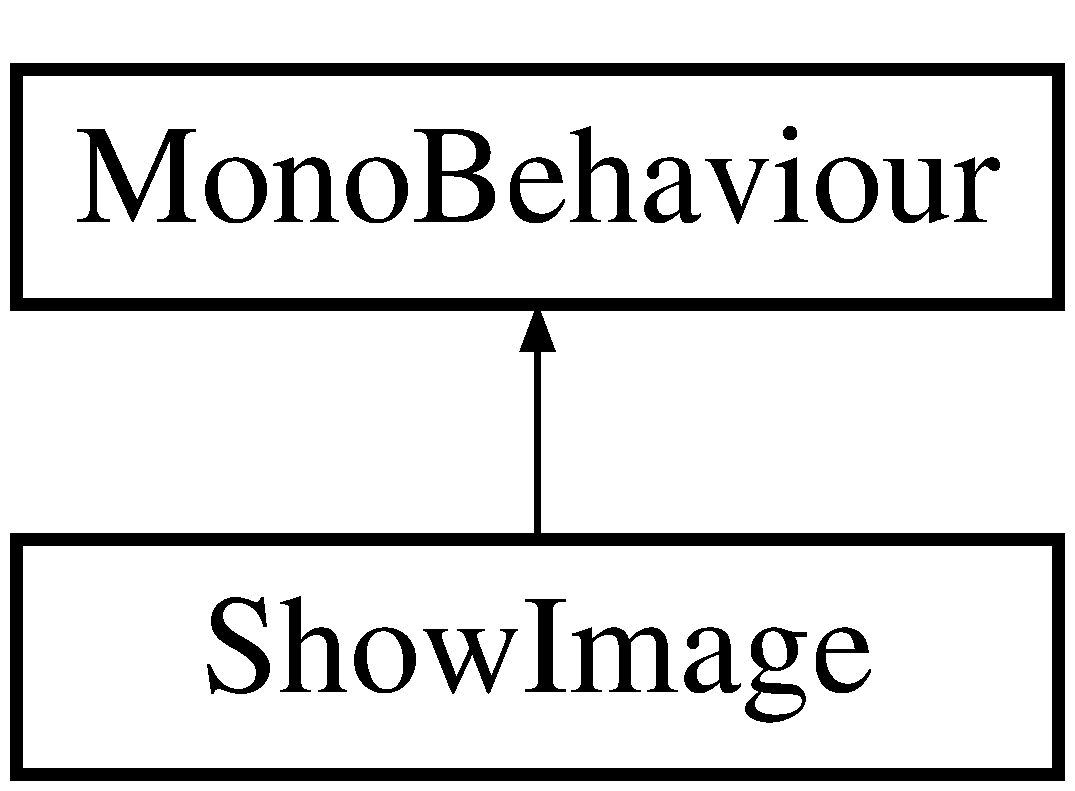
\includegraphics[height=2.000000cm]{class_show_image}
\end{center}
\end{figure}


The documentation for this class was generated from the following file\+:\begin{DoxyCompactItemize}
\item 
Assets/\+Scripts/\+Buttons/\mbox{\hyperlink{_show_image_8cs}{Show\+Image.\+cs}}\end{DoxyCompactItemize}

\hypertarget{class_stair_par}{}\section{Stair\+Par Class Reference}
\label{class_stair_par}\index{Stair\+Par@{Stair\+Par}}
Inheritance diagram for Stair\+Par\+:\begin{figure}[H]
\begin{center}
\leavevmode
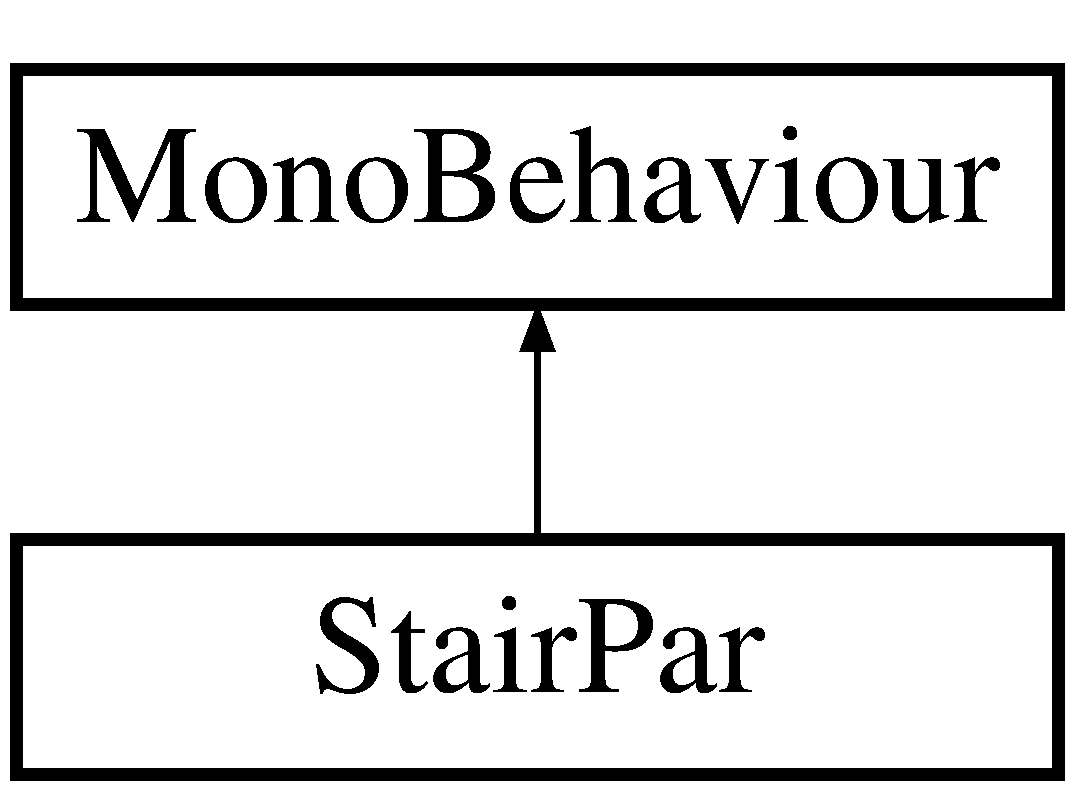
\includegraphics[height=2.000000cm]{class_stair_par}
\end{center}
\end{figure}
\subsection*{Public Attributes}
\begin{DoxyCompactItemize}
\item 
Transform \mbox{\hyperlink{class_stair_par_a15f91c7da18e2c921f656f61a1eaa4f1}{up}}
\end{DoxyCompactItemize}


\subsection{Member Data Documentation}
\mbox{\Hypertarget{class_stair_par_a15f91c7da18e2c921f656f61a1eaa4f1}\label{class_stair_par_a15f91c7da18e2c921f656f61a1eaa4f1}} 
\index{Stair\+Par@{Stair\+Par}!up@{up}}
\index{up@{up}!Stair\+Par@{Stair\+Par}}
\subsubsection{\texorpdfstring{up}{up}}
{\footnotesize\ttfamily Transform Stair\+Par.\+up}



The documentation for this class was generated from the following file\+:\begin{DoxyCompactItemize}
\item 
Assets/\+Scripts/\+Objects/\mbox{\hyperlink{_stair_par_8cs}{Stair\+Par.\+cs}}\end{DoxyCompactItemize}

\hypertarget{class_start_position}{}\section{Start\+Position Class Reference}
\label{class_start_position}\index{Start\+Position@{Start\+Position}}
Inheritance diagram for Start\+Position\+:\begin{figure}[H]
\begin{center}
\leavevmode
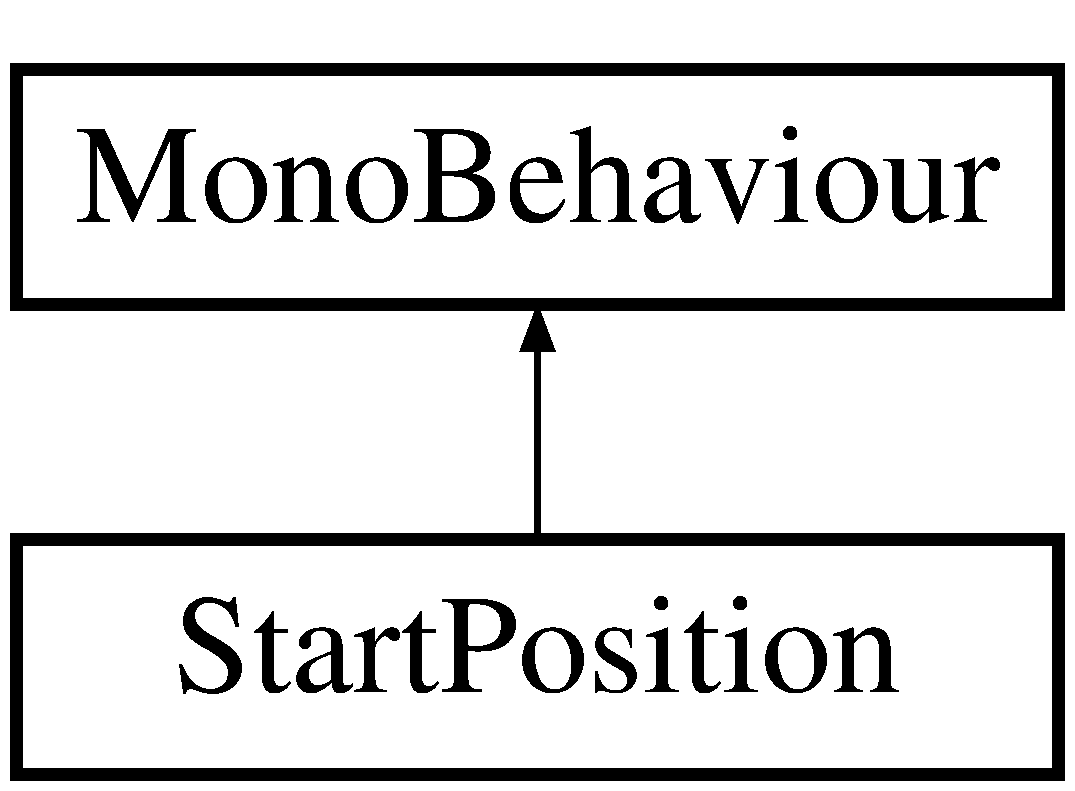
\includegraphics[height=2.000000cm]{class_start_position}
\end{center}
\end{figure}
\subsection*{Public Attributes}
\begin{DoxyCompactItemize}
\item 
Game\+Object \mbox{\hyperlink{class_start_position_a7f963cf576a350e488904e256930c040}{box}}
\end{DoxyCompactItemize}


\subsection{Member Data Documentation}
\mbox{\Hypertarget{class_start_position_a7f963cf576a350e488904e256930c040}\label{class_start_position_a7f963cf576a350e488904e256930c040}} 
\index{Start\+Position@{Start\+Position}!box@{box}}
\index{box@{box}!Start\+Position@{Start\+Position}}
\subsubsection{\texorpdfstring{box}{box}}
{\footnotesize\ttfamily Game\+Object Start\+Position.\+box}



The documentation for this class was generated from the following file\+:\begin{DoxyCompactItemize}
\item 
Assets/\+Scripts/\mbox{\hyperlink{_start_position_8cs}{Start\+Position.\+cs}}\end{DoxyCompactItemize}

\hypertarget{class_test}{}\section{Test Class Reference}
\label{class_test}\index{Test@{Test}}
Inheritance diagram for Test\+:\begin{figure}[H]
\begin{center}
\leavevmode
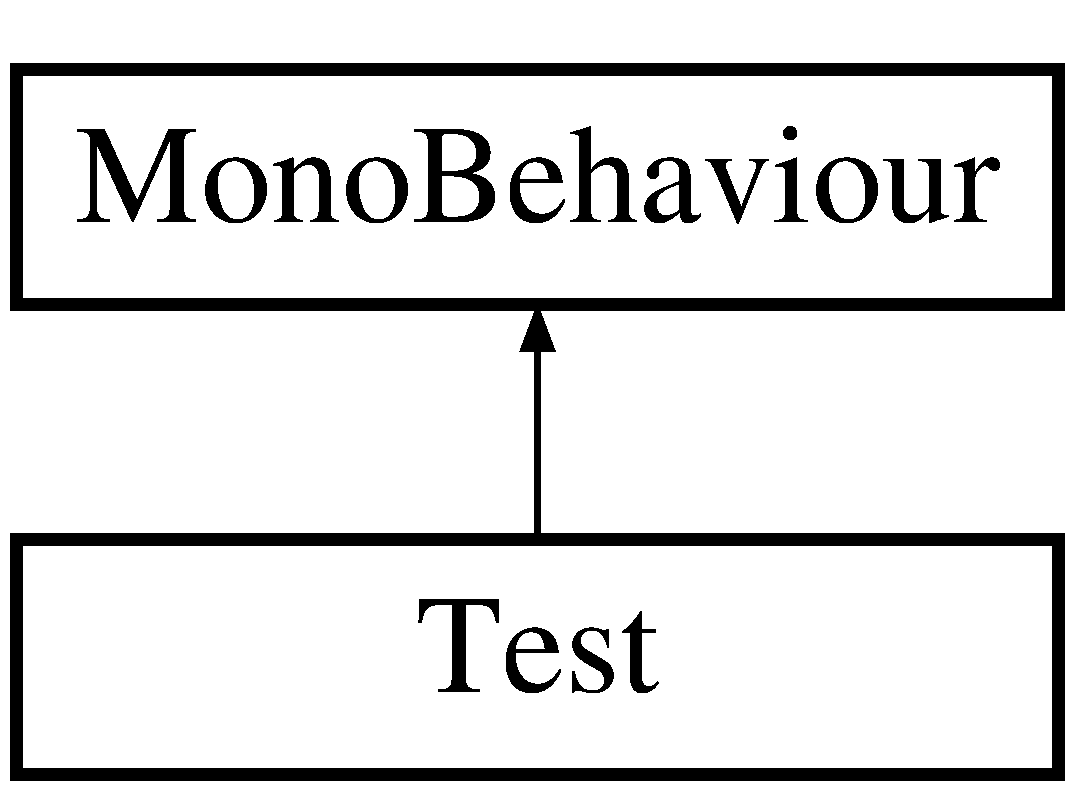
\includegraphics[height=2.000000cm]{class_test}
\end{center}
\end{figure}


The documentation for this class was generated from the following file\+:\begin{DoxyCompactItemize}
\item 
Assets/\+Scripts/\mbox{\hyperlink{_test_8cs}{Test.\+cs}}\end{DoxyCompactItemize}

\hypertarget{classthe_end_controller}{}\section{the\+End\+Controller Class Reference}
\label{classthe_end_controller}\index{the\+End\+Controller@{the\+End\+Controller}}
Inheritance diagram for the\+End\+Controller\+:\begin{figure}[H]
\begin{center}
\leavevmode
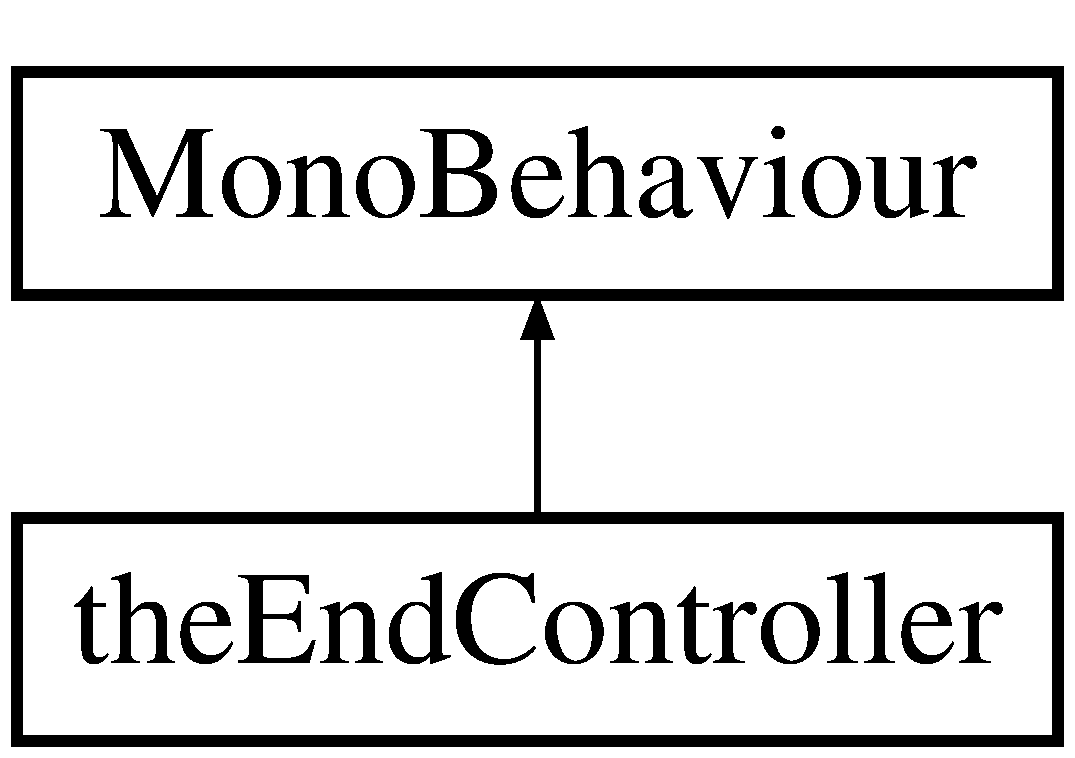
\includegraphics[height=2.000000cm]{classthe_end_controller}
\end{center}
\end{figure}


The documentation for this class was generated from the following file\+:\begin{DoxyCompactItemize}
\item 
Assets/\+Scripts/\+Objects/\mbox{\hyperlink{the_end_controller_8cs}{the\+End\+Controller.\+cs}}\end{DoxyCompactItemize}

\hypertarget{class_unit}{}\section{Unit Class Reference}
\label{class_unit}\index{Unit@{Unit}}
Inheritance diagram for Unit\+:\begin{figure}[H]
\begin{center}
\leavevmode
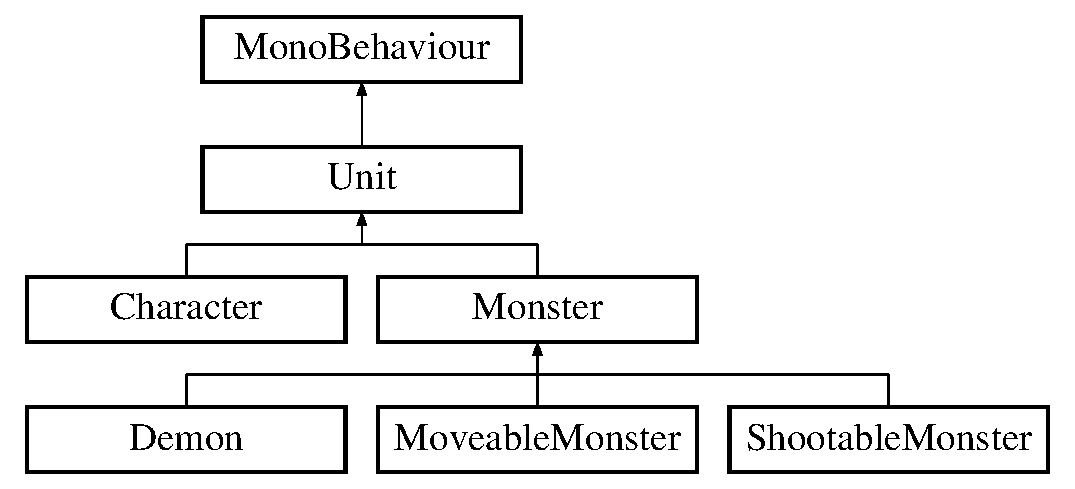
\includegraphics[height=4.000000cm]{class_unit}
\end{center}
\end{figure}
\subsection*{Public Member Functions}
\begin{DoxyCompactItemize}
\item 
virtual void \mbox{\hyperlink{class_unit_a698a459fd5eeef7fc906f4657b723fa4}{Receive\+Damage}} ()
\end{DoxyCompactItemize}
\subsection*{Protected Member Functions}
\begin{DoxyCompactItemize}
\item 
virtual void \mbox{\hyperlink{class_unit_af3d22541d2829f0de065bf6aecee9957}{Die}} ()
\end{DoxyCompactItemize}


\subsection{Member Function Documentation}
\mbox{\Hypertarget{class_unit_af3d22541d2829f0de065bf6aecee9957}\label{class_unit_af3d22541d2829f0de065bf6aecee9957}} 
\index{Unit@{Unit}!Die@{Die}}
\index{Die@{Die}!Unit@{Unit}}
\subsubsection{\texorpdfstring{Die()}{Die()}}
{\footnotesize\ttfamily virtual void Unit.\+Die (\begin{DoxyParamCaption}{ }\end{DoxyParamCaption})\hspace{0.3cm}{\ttfamily [inline]}, {\ttfamily [protected]}, {\ttfamily [virtual]}}

\mbox{\Hypertarget{class_unit_a698a459fd5eeef7fc906f4657b723fa4}\label{class_unit_a698a459fd5eeef7fc906f4657b723fa4}} 
\index{Unit@{Unit}!Receive\+Damage@{Receive\+Damage}}
\index{Receive\+Damage@{Receive\+Damage}!Unit@{Unit}}
\subsubsection{\texorpdfstring{Receive\+Damage()}{ReceiveDamage()}}
{\footnotesize\ttfamily virtual void Unit.\+Receive\+Damage (\begin{DoxyParamCaption}{ }\end{DoxyParamCaption})\hspace{0.3cm}{\ttfamily [inline]}, {\ttfamily [virtual]}}



Reimplemented in \mbox{\hyperlink{class_character_a4c92566bccf29f534c3863eb12fddba2}{Character}}, and \mbox{\hyperlink{class_demon_a90dc4738a3cab182e3daa2da35cbbbc6}{Demon}}.



The documentation for this class was generated from the following file\+:\begin{DoxyCompactItemize}
\item 
Assets/\+Scripts/\mbox{\hyperlink{_unit_8cs}{Unit.\+cs}}\end{DoxyCompactItemize}

\chapter{File Documentation}
\hypertarget{_button_manager_8cs}{}\section{Assets/\+Scripts/\+Buttons/\+Button\+Manager.cs File Reference}
\label{_button_manager_8cs}\index{Assets/\+Scripts/\+Buttons/\+Button\+Manager.\+cs@{Assets/\+Scripts/\+Buttons/\+Button\+Manager.\+cs}}
\subsection*{Classes}
\begin{DoxyCompactItemize}
\item 
class \mbox{\hyperlink{class_button_manager}{Button\+Manager}}
\end{DoxyCompactItemize}

\hypertarget{_new_game_button_8cs}{}\section{Assets/\+Scripts/\+Buttons/\+New\+Game\+Button.cs File Reference}
\label{_new_game_button_8cs}\index{Assets/\+Scripts/\+Buttons/\+New\+Game\+Button.\+cs@{Assets/\+Scripts/\+Buttons/\+New\+Game\+Button.\+cs}}
\subsection*{Classes}
\begin{DoxyCompactItemize}
\item 
class \mbox{\hyperlink{class_new_game_button}{New\+Game\+Button}}
\begin{DoxyCompactList}\small\item\em Класс, функция которого -\/ переход на следующую сцену \end{DoxyCompactList}\end{DoxyCompactItemize}

\hypertarget{_pause_8cs}{}\section{Assets/\+Scripts/\+Buttons/\+Pause.cs File Reference}
\label{_pause_8cs}\index{Assets/\+Scripts/\+Buttons/\+Pause.\+cs@{Assets/\+Scripts/\+Buttons/\+Pause.\+cs}}
\subsection*{Classes}
\begin{DoxyCompactItemize}
\item 
class \mbox{\hyperlink{class_pause}{Pause}}
\end{DoxyCompactItemize}

\hypertarget{_quit_8cs}{}\section{Assets/\+Scripts/\+Buttons/\+Quit.cs File Reference}
\label{_quit_8cs}\index{Assets/\+Scripts/\+Buttons/\+Quit.\+cs@{Assets/\+Scripts/\+Buttons/\+Quit.\+cs}}
\subsection*{Classes}
\begin{DoxyCompactItemize}
\item 
class \mbox{\hyperlink{class_quit}{Quit}}
\end{DoxyCompactItemize}

\hypertarget{_reload_8cs}{}\section{Assets/\+Scripts/\+Buttons/\+Reload.cs File Reference}
\label{_reload_8cs}\index{Assets/\+Scripts/\+Buttons/\+Reload.\+cs@{Assets/\+Scripts/\+Buttons/\+Reload.\+cs}}
\subsection*{Classes}
\begin{DoxyCompactItemize}
\item 
class \mbox{\hyperlink{class_reload}{Reload}}
\end{DoxyCompactItemize}

\hypertarget{_show_button_8cs}{}\section{Assets/\+Scripts/\+Buttons/\+Show\+Button.cs File Reference}
\label{_show_button_8cs}\index{Assets/\+Scripts/\+Buttons/\+Show\+Button.\+cs@{Assets/\+Scripts/\+Buttons/\+Show\+Button.\+cs}}
\subsection*{Classes}
\begin{DoxyCompactItemize}
\item 
class \mbox{\hyperlink{class_show_button}{Show\+Button}}
\end{DoxyCompactItemize}

\hypertarget{_show_image_8cs}{}\section{Assets/\+Scripts/\+Buttons/\+Show\+Image.cs File Reference}
\label{_show_image_8cs}\index{Assets/\+Scripts/\+Buttons/\+Show\+Image.\+cs@{Assets/\+Scripts/\+Buttons/\+Show\+Image.\+cs}}
\subsection*{Classes}
\begin{DoxyCompactItemize}
\item 
class \mbox{\hyperlink{class_show_image}{Show\+Image}}
\end{DoxyCompactItemize}

\hypertarget{_camera_controller_8cs}{}\section{Assets/\+Scripts/\+Camera/\+Camera\+Controller.cs File Reference}
\label{_camera_controller_8cs}\index{Assets/\+Scripts/\+Camera/\+Camera\+Controller.\+cs@{Assets/\+Scripts/\+Camera/\+Camera\+Controller.\+cs}}
\subsection*{Classes}
\begin{DoxyCompactItemize}
\item 
class \mbox{\hyperlink{class_camera_controller}{Camera\+Controller}}
\end{DoxyCompactItemize}

\hypertarget{_camera_follow2_d_8cs}{}\section{Assets/\+Scripts/\+Camera/\+Camera\+Follow2D.cs File Reference}
\label{_camera_follow2_d_8cs}\index{Assets/\+Scripts/\+Camera/\+Camera\+Follow2\+D.\+cs@{Assets/\+Scripts/\+Camera/\+Camera\+Follow2\+D.\+cs}}
\subsection*{Classes}
\begin{DoxyCompactItemize}
\item 
class \mbox{\hyperlink{class_camera_follow2_d}{Camera\+Follow2D}}
\end{DoxyCompactItemize}

\hypertarget{_character_8cs}{}\section{Assets/\+Scripts/\+Character.cs File Reference}
\label{_character_8cs}\index{Assets/\+Scripts/\+Character.\+cs@{Assets/\+Scripts/\+Character.\+cs}}
\subsection*{Classes}
\begin{DoxyCompactItemize}
\item 
class \mbox{\hyperlink{class_character}{Character}}
\end{DoxyCompactItemize}
\subsection*{Enumerations}
\begin{DoxyCompactItemize}
\item 
enum \mbox{\hyperlink{_character_8cs_a125875a194bc341fa32a233d963ffe02}{Char\+State}} \{ \mbox{\hyperlink{_character_8cs_a125875a194bc341fa32a233d963ffe02ae599161956d626eda4cb0a5ffb85271c}{Char\+State.\+Idle}}, 
\mbox{\hyperlink{_character_8cs_a125875a194bc341fa32a233d963ffe02ac5301693c4e792bcd5a479ef38fb8f8d}{Char\+State.\+Run}}, 
\mbox{\hyperlink{_character_8cs_a125875a194bc341fa32a233d963ffe02a101f693f72287a2819a364f64ca1c0ed}{Char\+State.\+Jump}}
 \}
\end{DoxyCompactItemize}


\subsection{Enumeration Type Documentation}
\mbox{\Hypertarget{_character_8cs_a125875a194bc341fa32a233d963ffe02}\label{_character_8cs_a125875a194bc341fa32a233d963ffe02}} 
\index{Character.\+cs@{Character.\+cs}!Char\+State@{Char\+State}}
\index{Char\+State@{Char\+State}!Character.\+cs@{Character.\+cs}}
\subsubsection{\texorpdfstring{Char\+State}{CharState}}
{\footnotesize\ttfamily enum \mbox{\hyperlink{_character_8cs_a125875a194bc341fa32a233d963ffe02}{Char\+State}}\hspace{0.3cm}{\ttfamily [strong]}}

\begin{DoxyEnumFields}{Enumerator}
\raisebox{\heightof{T}}[0pt][0pt]{\index{Idle@{Idle}!Character.\+cs@{Character.\+cs}}\index{Character.\+cs@{Character.\+cs}!Idle@{Idle}}}\mbox{\Hypertarget{_character_8cs_a125875a194bc341fa32a233d963ffe02ae599161956d626eda4cb0a5ffb85271c}\label{_character_8cs_a125875a194bc341fa32a233d963ffe02ae599161956d626eda4cb0a5ffb85271c}} 
Idle&\\
\hline

\raisebox{\heightof{T}}[0pt][0pt]{\index{Run@{Run}!Character.\+cs@{Character.\+cs}}\index{Character.\+cs@{Character.\+cs}!Run@{Run}}}\mbox{\Hypertarget{_character_8cs_a125875a194bc341fa32a233d963ffe02ac5301693c4e792bcd5a479ef38fb8f8d}\label{_character_8cs_a125875a194bc341fa32a233d963ffe02ac5301693c4e792bcd5a479ef38fb8f8d}} 
Run&\\
\hline

\raisebox{\heightof{T}}[0pt][0pt]{\index{Jump@{Jump}!Character.\+cs@{Character.\+cs}}\index{Character.\+cs@{Character.\+cs}!Jump@{Jump}}}\mbox{\Hypertarget{_character_8cs_a125875a194bc341fa32a233d963ffe02a101f693f72287a2819a364f64ca1c0ed}\label{_character_8cs_a125875a194bc341fa32a233d963ffe02a101f693f72287a2819a364f64ca1c0ed}} 
Jump&\\
\hline

\end{DoxyEnumFields}

\hypertarget{_chess_game_control_8cs}{}\section{Assets/\+Scripts/\+Chess\+Game/\+Chess\+Game\+Control.cs File Reference}
\label{_chess_game_control_8cs}\index{Assets/\+Scripts/\+Chess\+Game/\+Chess\+Game\+Control.\+cs@{Assets/\+Scripts/\+Chess\+Game/\+Chess\+Game\+Control.\+cs}}
\subsection*{Classes}
\begin{DoxyCompactItemize}
\item 
class \mbox{\hyperlink{class_chess_game_control}{Chess\+Game\+Control}}
\end{DoxyCompactItemize}

\hypertarget{_puzzle_8cs}{}\section{Assets/\+Scripts/\+Chess\+Game/\+Puzzle.cs File Reference}
\label{_puzzle_8cs}\index{Assets/\+Scripts/\+Chess\+Game/\+Puzzle.\+cs@{Assets/\+Scripts/\+Chess\+Game/\+Puzzle.\+cs}}
\subsection*{Classes}
\begin{DoxyCompactItemize}
\item 
class \mbox{\hyperlink{class_puzzle}{Puzzle}}
\end{DoxyCompactItemize}

\hypertarget{_demon_8cs}{}\section{Assets/\+Scripts/\+Demon.cs File Reference}
\label{_demon_8cs}\index{Assets/\+Scripts/\+Demon.\+cs@{Assets/\+Scripts/\+Demon.\+cs}}
\subsection*{Classes}
\begin{DoxyCompactItemize}
\item 
class \mbox{\hyperlink{class_demon}{Demon}}
\end{DoxyCompactItemize}

\hypertarget{empty_8cs}{}\section{Assets/\+Scripts/empty.cs File Reference}
\label{empty_8cs}\index{Assets/\+Scripts/empty.\+cs@{Assets/\+Scripts/empty.\+cs}}
\subsection*{Classes}
\begin{DoxyCompactItemize}
\item 
class \mbox{\hyperlink{classempty}{empty}}
\end{DoxyCompactItemize}

\hypertarget{fly_up_8cs}{}\section{Assets/\+Scripts/fly\+Up.cs File Reference}
\label{fly_up_8cs}\index{Assets/\+Scripts/fly\+Up.\+cs@{Assets/\+Scripts/fly\+Up.\+cs}}
\subsection*{Classes}
\begin{DoxyCompactItemize}
\item 
class \mbox{\hyperlink{classfly_up}{fly\+Up}}
\end{DoxyCompactItemize}

\hypertarget{_monster_8cs}{}\section{Assets/\+Scripts/\+Monsters/\+Monster.cs File Reference}
\label{_monster_8cs}\index{Assets/\+Scripts/\+Monsters/\+Monster.\+cs@{Assets/\+Scripts/\+Monsters/\+Monster.\+cs}}
\subsection*{Classes}
\begin{DoxyCompactItemize}
\item 
class \mbox{\hyperlink{class_monster}{Monster}}
\end{DoxyCompactItemize}

\hypertarget{_moveable_monster_8cs}{}\section{Assets/\+Scripts/\+Monsters/\+Moveable\+Monster.cs File Reference}
\label{_moveable_monster_8cs}\index{Assets/\+Scripts/\+Monsters/\+Moveable\+Monster.\+cs@{Assets/\+Scripts/\+Monsters/\+Moveable\+Monster.\+cs}}
\subsection*{Classes}
\begin{DoxyCompactItemize}
\item 
class \mbox{\hyperlink{class_moveable_monster}{Moveable\+Monster}}
\end{DoxyCompactItemize}

\hypertarget{_obstacle_8cs}{}\section{Assets/\+Scripts/\+Monsters/\+Obstacle.cs File Reference}
\label{_obstacle_8cs}\index{Assets/\+Scripts/\+Monsters/\+Obstacle.\+cs@{Assets/\+Scripts/\+Monsters/\+Obstacle.\+cs}}
\subsection*{Classes}
\begin{DoxyCompactItemize}
\item 
class \mbox{\hyperlink{class_obstacle}{Obstacle}}
\end{DoxyCompactItemize}

\hypertarget{_shootable_monster_8cs}{}\section{Assets/\+Scripts/\+Monsters/\+Shootable\+Monster.cs File Reference}
\label{_shootable_monster_8cs}\index{Assets/\+Scripts/\+Monsters/\+Shootable\+Monster.\+cs@{Assets/\+Scripts/\+Monsters/\+Shootable\+Monster.\+cs}}
\subsection*{Classes}
\begin{DoxyCompactItemize}
\item 
class \mbox{\hyperlink{class_shootable_monster}{Shootable\+Monster}}
\end{DoxyCompactItemize}

\hypertarget{_box_8cs}{}\section{Assets/\+Scripts/\+Objects/\+Box.cs File Reference}
\label{_box_8cs}\index{Assets/\+Scripts/\+Objects/\+Box.\+cs@{Assets/\+Scripts/\+Objects/\+Box.\+cs}}
\subsection*{Classes}
\begin{DoxyCompactItemize}
\item 
class \mbox{\hyperlink{class_box}{Box}}
\end{DoxyCompactItemize}

\hypertarget{_box_shield_8cs}{}\section{Assets/\+Scripts/\+Objects/\+Box\+Shield.cs File Reference}
\label{_box_shield_8cs}\index{Assets/\+Scripts/\+Objects/\+Box\+Shield.\+cs@{Assets/\+Scripts/\+Objects/\+Box\+Shield.\+cs}}
\subsection*{Classes}
\begin{DoxyCompactItemize}
\item 
class \mbox{\hyperlink{class_box_shield}{Box\+Shield}}
\end{DoxyCompactItemize}

\hypertarget{_bullet_8cs}{}\section{Assets/\+Scripts/\+Objects/\+Bullet.cs File Reference}
\label{_bullet_8cs}\index{Assets/\+Scripts/\+Objects/\+Bullet.\+cs@{Assets/\+Scripts/\+Objects/\+Bullet.\+cs}}
\subsection*{Classes}
\begin{DoxyCompactItemize}
\item 
class \mbox{\hyperlink{class_bullet}{Bullet}}
\end{DoxyCompactItemize}

\hypertarget{_door_trigger_8cs}{}\section{Assets/\+Scripts/\+Objects/\+Door\+Trigger.cs File Reference}
\label{_door_trigger_8cs}\index{Assets/\+Scripts/\+Objects/\+Door\+Trigger.\+cs@{Assets/\+Scripts/\+Objects/\+Door\+Trigger.\+cs}}
\subsection*{Classes}
\begin{DoxyCompactItemize}
\item 
class \mbox{\hyperlink{class_door_trigger}{Door\+Trigger}}
\end{DoxyCompactItemize}

\hypertarget{fly_platform_8cs}{}\section{Assets/\+Scripts/\+Objects/fly\+Platform.cs File Reference}
\label{fly_platform_8cs}\index{Assets/\+Scripts/\+Objects/fly\+Platform.\+cs@{Assets/\+Scripts/\+Objects/fly\+Platform.\+cs}}
\subsection*{Classes}
\begin{DoxyCompactItemize}
\item 
class \mbox{\hyperlink{classfly_platform}{fly\+Platform}}
\end{DoxyCompactItemize}

\hypertarget{_heart_8cs}{}\section{Assets/\+Scripts/\+Objects/\+Heart.cs File Reference}
\label{_heart_8cs}\index{Assets/\+Scripts/\+Objects/\+Heart.\+cs@{Assets/\+Scripts/\+Objects/\+Heart.\+cs}}
\subsection*{Classes}
\begin{DoxyCompactItemize}
\item 
class \mbox{\hyperlink{class_heart}{Heart}}
\end{DoxyCompactItemize}

\hypertarget{_ice_platform_8cs}{}\section{Assets/\+Scripts/\+Objects/\+Ice\+Platform.cs File Reference}
\label{_ice_platform_8cs}\index{Assets/\+Scripts/\+Objects/\+Ice\+Platform.\+cs@{Assets/\+Scripts/\+Objects/\+Ice\+Platform.\+cs}}
\subsection*{Classes}
\begin{DoxyCompactItemize}
\item 
class \mbox{\hyperlink{class_ice_platform}{Ice\+Platform}}
\end{DoxyCompactItemize}

\hypertarget{_lever1_8cs}{}\section{Assets/\+Scripts/\+Objects/\+Lever1.cs File Reference}
\label{_lever1_8cs}\index{Assets/\+Scripts/\+Objects/\+Lever1.\+cs@{Assets/\+Scripts/\+Objects/\+Lever1.\+cs}}
\subsection*{Classes}
\begin{DoxyCompactItemize}
\item 
class \mbox{\hyperlink{class_lever1}{Lever1}}
\end{DoxyCompactItemize}

\hypertarget{_lives_bar_8cs}{}\section{Assets/\+Scripts/\+Objects/\+Lives\+Bar.cs File Reference}
\label{_lives_bar_8cs}\index{Assets/\+Scripts/\+Objects/\+Lives\+Bar.\+cs@{Assets/\+Scripts/\+Objects/\+Lives\+Bar.\+cs}}
\subsection*{Classes}
\begin{DoxyCompactItemize}
\item 
class \mbox{\hyperlink{class_lives_bar}{Lives\+Bar}}
\end{DoxyCompactItemize}

\hypertarget{_moving_object_8cs}{}\section{Assets/\+Scripts/\+Objects/\+Moving\+Object.cs File Reference}
\label{_moving_object_8cs}\index{Assets/\+Scripts/\+Objects/\+Moving\+Object.\+cs@{Assets/\+Scripts/\+Objects/\+Moving\+Object.\+cs}}
\subsection*{Classes}
\begin{DoxyCompactItemize}
\item 
class \mbox{\hyperlink{class_moving_object}{Moving\+Object}}
\end{DoxyCompactItemize}

\hypertarget{_portal_8cs}{}\section{Assets/\+Scripts/\+Objects/\+Portal.cs File Reference}
\label{_portal_8cs}\index{Assets/\+Scripts/\+Objects/\+Portal.\+cs@{Assets/\+Scripts/\+Objects/\+Portal.\+cs}}
\subsection*{Classes}
\begin{DoxyCompactItemize}
\item 
class \mbox{\hyperlink{class_portal}{Portal}}
\end{DoxyCompactItemize}
\subsection*{Enumerations}
\begin{DoxyCompactItemize}
\item 
enum \mbox{\hyperlink{_portal_8cs_a8f6e870ae9fd45ccd4f8e70fa5b07aa6}{Portal\+State}} \{ \mbox{\hyperlink{_portal_8cs_a8f6e870ae9fd45ccd4f8e70fa5b07aa6a75237bde6f9a409fcd4eb5c2b9d944ee}{Portal\+State.\+Meet\+Player}}, 
\mbox{\hyperlink{_portal_8cs_a8f6e870ae9fd45ccd4f8e70fa5b07aa6a1b4c94af1f4a8b32bb59576ba207244d}{Portal\+State.\+Wait\+Player}}, 
\mbox{\hyperlink{_portal_8cs_a8f6e870ae9fd45ccd4f8e70fa5b07aa6aea1b3a8db0921508340191b57b67e809}{Portal\+State.\+Bring\+Player}}
 \}
\end{DoxyCompactItemize}


\subsection{Enumeration Type Documentation}
\mbox{\Hypertarget{_portal_8cs_a8f6e870ae9fd45ccd4f8e70fa5b07aa6}\label{_portal_8cs_a8f6e870ae9fd45ccd4f8e70fa5b07aa6}} 
\index{Portal.\+cs@{Portal.\+cs}!Portal\+State@{Portal\+State}}
\index{Portal\+State@{Portal\+State}!Portal.\+cs@{Portal.\+cs}}
\subsubsection{\texorpdfstring{Portal\+State}{PortalState}}
{\footnotesize\ttfamily enum \mbox{\hyperlink{_portal_8cs_a8f6e870ae9fd45ccd4f8e70fa5b07aa6}{Portal\+State}}\hspace{0.3cm}{\ttfamily [strong]}}

\begin{DoxyEnumFields}{Enumerator}
\raisebox{\heightof{T}}[0pt][0pt]{\index{Meet\+Player@{Meet\+Player}!Portal.\+cs@{Portal.\+cs}}\index{Portal.\+cs@{Portal.\+cs}!Meet\+Player@{Meet\+Player}}}\mbox{\Hypertarget{_portal_8cs_a8f6e870ae9fd45ccd4f8e70fa5b07aa6a75237bde6f9a409fcd4eb5c2b9d944ee}\label{_portal_8cs_a8f6e870ae9fd45ccd4f8e70fa5b07aa6a75237bde6f9a409fcd4eb5c2b9d944ee}} 
Meet\+Player&\\
\hline

\raisebox{\heightof{T}}[0pt][0pt]{\index{Wait\+Player@{Wait\+Player}!Portal.\+cs@{Portal.\+cs}}\index{Portal.\+cs@{Portal.\+cs}!Wait\+Player@{Wait\+Player}}}\mbox{\Hypertarget{_portal_8cs_a8f6e870ae9fd45ccd4f8e70fa5b07aa6a1b4c94af1f4a8b32bb59576ba207244d}\label{_portal_8cs_a8f6e870ae9fd45ccd4f8e70fa5b07aa6a1b4c94af1f4a8b32bb59576ba207244d}} 
Wait\+Player&\\
\hline

\raisebox{\heightof{T}}[0pt][0pt]{\index{Bring\+Player@{Bring\+Player}!Portal.\+cs@{Portal.\+cs}}\index{Portal.\+cs@{Portal.\+cs}!Bring\+Player@{Bring\+Player}}}\mbox{\Hypertarget{_portal_8cs_a8f6e870ae9fd45ccd4f8e70fa5b07aa6aea1b3a8db0921508340191b57b67e809}\label{_portal_8cs_a8f6e870ae9fd45ccd4f8e70fa5b07aa6aea1b3a8db0921508340191b57b67e809}} 
Bring\+Player&\\
\hline

\end{DoxyEnumFields}

\hypertarget{_stair_par_8cs}{}\section{Assets/\+Scripts/\+Objects/\+Stair\+Par.cs File Reference}
\label{_stair_par_8cs}\index{Assets/\+Scripts/\+Objects/\+Stair\+Par.\+cs@{Assets/\+Scripts/\+Objects/\+Stair\+Par.\+cs}}
\subsection*{Classes}
\begin{DoxyCompactItemize}
\item 
class \mbox{\hyperlink{class_stair_par}{Stair\+Par}}
\end{DoxyCompactItemize}

\hypertarget{the_end_controller_8cs}{}\section{Assets/\+Scripts/\+Objects/the\+End\+Controller.cs File Reference}
\label{the_end_controller_8cs}\index{Assets/\+Scripts/\+Objects/the\+End\+Controller.\+cs@{Assets/\+Scripts/\+Objects/the\+End\+Controller.\+cs}}
\subsection*{Classes}
\begin{DoxyCompactItemize}
\item 
class \mbox{\hyperlink{classthe_end_controller}{the\+End\+Controller}}
\end{DoxyCompactItemize}

\hypertarget{_ornament_8cs}{}\section{Assets/\+Scripts/\+Puzzle\+Game/\+Ornament.cs File Reference}
\label{_ornament_8cs}\index{Assets/\+Scripts/\+Puzzle\+Game/\+Ornament.\+cs@{Assets/\+Scripts/\+Puzzle\+Game/\+Ornament.\+cs}}
\subsection*{Classes}
\begin{DoxyCompactItemize}
\item 
class \mbox{\hyperlink{class_ornament}{Ornament}}
\end{DoxyCompactItemize}

\hypertarget{_ornament_manager_8cs}{}\section{Assets/\+Scripts/\+Puzzle\+Game/\+Ornament\+Manager.cs File Reference}
\label{_ornament_manager_8cs}\index{Assets/\+Scripts/\+Puzzle\+Game/\+Ornament\+Manager.\+cs@{Assets/\+Scripts/\+Puzzle\+Game/\+Ornament\+Manager.\+cs}}
\subsection*{Classes}
\begin{DoxyCompactItemize}
\item 
class \mbox{\hyperlink{class_ornament_manager}{Ornament\+Manager}}
\end{DoxyCompactItemize}

\hypertarget{_shield_8cs}{}\section{Assets/\+Scripts/\+Shield.cs File Reference}
\label{_shield_8cs}\index{Assets/\+Scripts/\+Shield.\+cs@{Assets/\+Scripts/\+Shield.\+cs}}
\subsection*{Classes}
\begin{DoxyCompactItemize}
\item 
class \mbox{\hyperlink{class_shield}{Shield}}
\end{DoxyCompactItemize}

\hypertarget{_start_position_8cs}{}\section{Assets/\+Scripts/\+Start\+Position.cs File Reference}
\label{_start_position_8cs}\index{Assets/\+Scripts/\+Start\+Position.\+cs@{Assets/\+Scripts/\+Start\+Position.\+cs}}
\subsection*{Classes}
\begin{DoxyCompactItemize}
\item 
class \mbox{\hyperlink{class_start_position}{Start\+Position}}
\end{DoxyCompactItemize}

\hypertarget{_test_8cs}{}\section{Assets/\+Scripts/\+Test.cs File Reference}
\label{_test_8cs}\index{Assets/\+Scripts/\+Test.\+cs@{Assets/\+Scripts/\+Test.\+cs}}
\subsection*{Classes}
\begin{DoxyCompactItemize}
\item 
class \mbox{\hyperlink{class_test}{Test}}
\end{DoxyCompactItemize}

\hypertarget{_unit_8cs}{}\section{Assets/\+Scripts/\+Unit.cs File Reference}
\label{_unit_8cs}\index{Assets/\+Scripts/\+Unit.\+cs@{Assets/\+Scripts/\+Unit.\+cs}}
\subsection*{Classes}
\begin{DoxyCompactItemize}
\item 
class \mbox{\hyperlink{class_unit}{Unit}}
\end{DoxyCompactItemize}

%--- End generated contents ---

% Index
\backmatter
\newpage
\phantomsection
\clearemptydoublepage
\addcontentsline{toc}{chapter}{Index}
\printindex

\end{document}
